\documentclass{report}
\usepackage[utf8]{inputenc}
\usepackage[russian]{babel}
\usepackage{setspace,amsmath}
\usepackage{amssymb}
\usepackage{amsthm}
\usepackage{amsfonts}
\usepackage{scalerel}
\usepackage{graphicx}
\usepackage{float}
\usepackage{wrapfig}
\usepackage[unicode, pdftex]{hyperref}

\def\stretchint#1{\vcenter{\hbox{\stretchto[440]{\displaystyle\int}{#1}}}}
\def\scaleint#1{\vcenter{\hbox{\scaleto[3ex]{\displaystyle\int}{#1}}}}

\theoremstyle{definition}
\newtheorem{definition}{Определение}[section]
\newtheorem{example}{Пример}
\newtheorem*{effect}{Следствие}
\newtheorem{statement}{Утверждение}[section]
\newtheorem*{remark}{Замечание}
\newtheorem{lemma}{Лемма}[section]
\newtheorem{theorem}{Теорема}[section]

\title{Математический Анализ \\ 2 семестр}
\author{Данил Заблоцкий}
\date{\today}

\begin{document}

\maketitle
\tableofcontents
\chapter{Дифференциальное исчисление}

\section{Формула Тейлора}

\subsection{Формула Тейлора с остаточным членом в форме Пеано}

Пусть $f:(a;b)\rightarrow\mathbb{R}, \ x_0 \in (a;b)$. Нужно построить многочлен $P(x;x_0)$ вида:
\begin{equation*}
  P(x;x_0)=a_0 + a_1(x-x_0) + a_2(x-x_0)^2 + \ldots + a_n (x-x_0)^n
\end{equation*}
$f(x) - P(x;x_0) = r_n (x;x_0)$ - $n$-ый остаточный член в формуле Тейлора.

\begin{definition}
  Остаточные члены в форме Пеано имеют вид:
  \begin{equation*}
    r_n(x;x_0) = \underset{x\rightarrow x_0}{o}((x-x_0)^n)
  \end{equation*}
\end{definition}

\begin{definition}
  Пусть $f:(a;b)\rightarrow\mathbb{R}, \ x_0\in(a;b), \ f(x)$ имеет в точке $x_0$ проиводные до
  $n$-ого порядка включительно.

  \textbf{Многочленом Тейлора} (полиномом Тейлора) функции $f(x)$ в точке $x$ называется многочлен:
  \begin{equation*}
    P(x;x_0) = f(x_0) + \frac{f'(x_0)}{1!}(x-x_0) + \frac{f''(x_0)}{2!}(x-x_0)^2 + \ldots +
    + \frac{f^{(n)}(x_0)}{n!}(x-x_0)^n
  \end{equation*}
\end{definition}


\begin{statement}
  Если $f:(a;b)\rightarrow\mathbb{R}$ имеет в точке $x_0\in(a;b)$ производные до $n$-го порядка
  включительно и $P(x;x_0)$ - ее многочлен Тейлора, то:
  \begin{equation*}
    f(x_0) = P(x_0;x_0), \ f'(x_0) = P'(x_0;x_0), \ \ldots, \ f^{(n)}(x_0) = P^{(n)}(x_0;x_0)
  \end{equation*}
\end{statement}

\begin{proof}
  $P(x;x_0) = f(x) + \ldots + \frac{f^{(n)}(x_0)}{n!}(x-x_0)^n$, при $x = x_0$: $P(x_0;x_0) = f(x_0)$

  $P'(x;x_0) = + \frac{f'(x_0)}{1!}(x-x_0) + \frac{f''(x_0)}{2!}2(x-x_0) + \ldots
    + \frac{f^{(n)}(x_0)}{n!}n(x-x_0)^{n-1}$, при $x = x_0$: $P'(x_0;x_0) = \frac{f'(x_0)}{1!}; \
    P''(x;x_0) = f''(x_0) + \frac{f'''(x_0)}{3!}6(x-x_0) + \ldots + \frac{f^{(n)}(x_0)}{n!}
    n(n-1)(x-x_0)^{n-2}; \ P^{(n)}(x_0;x_0) = f^{(n)}(x_0)$.
\end{proof}

\begin{theorem}
  Пусть $f:(a;b)\rightarrow\mathbb{R}, \ x_0\in(a;b), \ f$ имеет в точке $x_0$ проивзодные до $n$-ого
  порядка включительно, тогда существует единственный многочлен вида:
  \begin{equation*}
    p(x;x_0) = a_0 + a_1(x-x_0) + \ldots + a_n(x-x_0)^n
  \end{equation*}
  такой, что:
  \begin{equation*}
    f(x) - P(x;x_0) = \underset{x\rightarrow x_0}{o}((x-x_0)^n)
  \end{equation*}
\end{theorem}

\begin{proof}
  (теоремы)
  \begin{enumerate}
    \item Докажем единственность.

          Пусть $Q(x;x_0) = b_0 + b_1(x-x_0) + \ldots + b_n(x-x_0)^n: \ f(x) - Q(x;x_0) = \underset{x\rightarrow
            x_0}{o}((x-x_0)^n), \ f(x) = P(x;x_0) + \underset{x\rightarrow x_0}{o}((x-x_0)^n)$.

          Рассмотрим разность этих выражений: $f(x) - f(x) = P(x;x_0) - Q(x;x_0) + \underset{x\rightarrow x_0}
            {o}((x-x_0)^n) = (a_0 - b_0) + (a_1 - b_1)(x-x_0) + (a_2 - b_2)(x-x_0)^2 + \ldots + (a_n - b_n)
            (x-x_0)^n + \underset{x\rightarrow x_0}{o}((x-x_0)^n)$ (*).

          Переходя к пределу при $x\rightarrow x_0$, получим, что $0 = a_0 - b_0 \implies a_0 = b_0$. Разделим
          (*) на $x-x_0: \ 0 = (a_1 - b_1) + (a_2 - b_2)(x-x_0) + \ldots + (a_n - b_n)(x-x_0)^{n-1} +
            \underset{x\rightarrow x_0}{o}((x-x_0)^{n-1})$ (**);
          \begin{equation*}
            \underset{x\rightarrow x_0}{o}((x-x_0)^{n}) = \alpha(x)(x-x_0)^n, \
            \alpha(x)\rightarrow0 \ (x\rightarrow x_0)
          \end{equation*}
          Переходя к пределу при $x\rightarrow x_0$ в (**) получаем, что $a_1 - b_1 = 0 \implies a_1 = b_1$.
          Используя ММИ можно показать, что $a_i = b_i, \ i = 2,\ldots,n \implies Q(x;x_0) = P(x;x_0)$.
    \item Докажем существование.

          \begin{lemma}
            Если фукнция $\phi:(a;b)\rightarrow\mathbb{R}, \ x_0\in(a;b)$, такая, что $\phi(x_0) = \phi'(x_0)
              = \ldots = \phi^{(n)}(x_0) = 0$ ($\phi(x)$ имеет производную до $n$-ого порядка включительно),
            причем все производные непрерывны в некоторой окрестности точки $x_0$. Тогда:
            \begin{equation*}
              \phi(x) = \underset{x\rightarrow x_0}{o}((x-x_0)^n), \ (x\rightarrow x_0)
            \end{equation*}
          \end{lemma}
          Допустим, что лемма доказана. Тогда положим $\phi(x) = f(x) - P(x;x_0)$, тогда будет выполнено
          условие леммы (+ смотри утверждение в начале параграфа) $\implies f(x) - P(x;x_0) =
            \underset{x\rightarrow x_0}{o}((x-x_0)^n)$ при $x\rightarrow x_0$, где $P(x;x_0)$ -
          многочлен Тейлора функциии $f$ в точке $x_0$.
  \end{enumerate}
\end{proof}

\clearpage

\begin{proof}
  (леммы)

  По индукции.

  Пусть $n = 1$, то есть $\phi$ - дифференцируема в окрестности точки $x_0$ и $\phi(x_0)
    = \phi'(x_0) = 0$. Тогда $\phi(x) = \phi(x) - \phi(x_0) = \phi'(\xi)(x-x_0)$, где $\xi\in(a;b)$
  (по теореме Лагранжа).

  Далее, $\phi'(\xi)\rightarrow\phi'(x_0)$ при $\xi\rightarrow x_0$ (используя непрерывность функции)
  $\implies \phi'(\xi)$ - бесконечно малая, поскольку $\phi'(x_0) = 0$.

  То есть $\phi'(\xi)\rightarrow0$ при $\xi\rightarrow x_0 \implies \phi(x) = \phi'(\xi)(x-x_0) =
    \underset{\xi\rightarrow x_0}{o}(x-x_0)$.

  Допустим, лемма верна для $k=n-1$. Положим $g(x) = \phi'(x)$. Тогда $g(x)$ имеет непрерывные производные
  до $(n-1)$-ого порядка включительно, при этом $g(x_0) = g'(x_0) = \ldots = g^{(n)}(x_0) = 0 \implies$
  по утверждению леммы:
  \begin{equation*}
    g(x) = \underset{x\rightarrow x_0}{o}((x-x_0)^{n-1})
  \end{equation*}

  Далее, $\phi(x) - \phi(x_0) = \phi(x) = \phi'(\xi)(x-x_0) = g(\xi)(x-x_0) = \underset{\xi\rightarrow x_0}
    {o}((\xi - x_0)^{n-1})(x-x_0) = \alpha(\xi)(\xi - x_0)^{n-1}(x-x_0), \ \alpha(\xi)\rightarrow 0$ при
  $\xi \rightarrow x_0$.

  Отсюда $| \phi(x) | = | \alpha(\xi) | | \xi - x_0 |^{n-1} | x - x_0 | \leqslant | \alpha (\xi) |
    | x - x_0 |^n$ ($\alpha (\xi) \rightarrow0$ при $\xi \rightarrow x_0$) $\implies \phi(x) = \underset
    {x\rightarrow x_0}{o}((x-x_0)^n)$.
\end{proof}

\subsection*{Примеры представления некоторых функций через многочлен Тейлора ($x_0 = 0$)}

\begin{enumerate}
  \item $e^x = 1 + x + \frac{x^2}{2} + \frac{x^3}{3!} + \ldots + \frac{x^n}{n!} + \underset{x\rightarrow0}
          {o}(x^n)$
  \item $\sin x = x - \frac{x^3}{3!} + \frac{x^5}{5!} - \ldots + (-1)^{n-1}\frac{x^{2n+1}}{(2n+1)!} +
          \underset{x\rightarrow0}{o}(x^{2n-1})$
  \item $\cos x = 1 - \frac{x^2}{2} + \frac{x^4}{4!} - \ldots + (-1)^n\frac{x^{2n}}{(2n)!} +
          \underset{x\rightarrow0}{o}(x^{2n})$
  \item $\ln (1+x) = x - \frac{x^2}{2} + \frac{x^3}{3!} - \ldots + (-1)^{n-1}\frac{x^n}{n!} +
          \underset{x\rightarrow0}{o}(x^n)$
  \item $(1+x)^\alpha = 1 + \alpha x + \frac{\alpha (\alpha - 1)}{\alpha !} x^2 + \ldots +
          \frac{\alpha(\alpha-1)(\alpha-2)\ldots(\alpha - (n-1))}{n!}x^n + \underset{x\rightarrow0}{o}(x^n)$
\end{enumerate}

\subsection{Формула Тейлора с остаточным членом в форме Лагранжа и в форме Коши}



\section{Приложения дифференциального исчисления}

\subsection{Монотонность функции}



\subsection{Экстремумы}



\subsection{Выпуклость функции}

\subsection*{Геометрический смысл выпуклой функции}




\section{Первообразная и неопределенный интеграл}

\begin{definition}[Первообразная функция]
  Пусть \(X\) - промежуток, \(f:X\rightarrow \mathbb{R}\). Функция \(F(x)\) называется
  \textbf{первообразной} \(f(x)\), если производная \(F'(x) = f(x)\), при этом \(F(x)\)
  дифференцируема и непрерывна.
\end{definition}

\begin{example}
  \(f(x) = 2x \implies F(x) = x^{2}\). В самом деле, \(F'(x) = f(x)\).
\end{example}

\begin{statement}
  (О первообразной)
  \begin{enumerate}
    \item Если \(F(x)\) - первообразная функции \(f(x)\) на промежутке \(X\), и
          \(\varPhi(x) = F(x) + C, \ c \in \mathbb{R}\), то \(\varPhi(x)\) - тоже первообразная.
    \item Если \(F(x)\) и \(\varPhi(x)\) - две первообразные для \(f(x)\) на промежутке \(X\),
          то \(\exists C = const, \ c \in \mathbb{R}\) такая, что \(\varPhi(x) = F(x) + C\).
  \end{enumerate}
\end{statement}

\begin{proof}
  (Утверждения о первообразной)
  \begin{enumerate}
    \item \(\Phi'(x) = (F(x) + C)' = F'(x) = f(x) \implies \Phi(x)\)
          - первообразная для \(f(x)\).
    \item Так как \(F(x)\) и \(\Phi(x)\) - первообразные для \(f(x)\), то \(F'(x) = f(x),
          \Phi'(x) = f(x)\). Рассмотрим функцию \(\phi = \Phi(x) - F(x), \ \forall x \in X\):
          \(\phi'(x) = \Phi'(x) - F'(x) = f(x) - f(x) = 0\). Рассмотрим
          \(\forall x_{1}, x_{2} \in X\), по теореме Лагранжа, \(\exists \xi \in (x_{1}, x_{2}):
          \ \phi(x_{1}) - \phi(x_{2}) = \phi'(\xi)(x_{1} - x_{2}) = 0 \implies \phi(x_{1}) =
          \phi(x_{2}) \implies \phi(x) = const\) для \(\forall x \in X\).
  \end{enumerate}
\end{proof}

\begin{definition}[Неопределенный интеграл]
  Совокупность всех первообразных для функции \(f(x)\) на промежутке \(X\) называется
  \textbf{неопределенным интегралом} и обозначается:
  \begin{equation*}
    \int f(x) dx
  \end{equation*}
  Таким образом, \(\int f(x) dx = \{F(x) + C\), где \(F'(x) = f(x), \ C \in \mathbb{R}\}\),
  или:
  \begin{equation*}
    \int f(x) dx = F(x) + C
  \end{equation*}
\end{definition}

\begin{remark}
  (Для неопределенного интеграла)
  \begin{itemize}
    \item \((\int f(x) dx)_{x}' = (F(x) + C)_{x}' = F'(x) = f(x)\);
    \item \(d(\int f(x) dx) = d(F(x) + C) = (F(x) + C)' dx = F'(x) dx = f(x) dx\);
    \item \(\int d(F(x)) = \int F'(x) dx = \int f(x) dx = F(x) + C, \ C \in \mathbb{R}\).
  \end{itemize}
\end{remark}

\begin{definition}[интегрирование]
  Операция нахождения первообразной функции \(f(x)\) называется ее \textbf{интегрированием}.
\end{definition}

\begin{statement}
  (Основные методы интегрирования) \\
  Пусть \(f: X \rightarrow \mathbb{R}, \ g:X \rightarrow \mathbb{R}, \ X\) - промежуток:
  \begin{enumerate}
    \item Пусть \(\alpha, \beta \in \mathbb{R} = const\), тогда:\\
          \(\int (\alpha f(x) + \beta g(x)) dx = \alpha \int f(x) dx + \beta \int g(x) dx\).
    \item Формула интегрирования по частям: \\
          \(udv = uv - \int udv, \ u = u(x), v = v(x)\).
    \item Интегрирование подстановкой: \\
          Пусть \(T\) - промежуток, \(X = X(t)\) - дифференцируема на \(T\). \\
          Тогда \(\int f(X(t)) * X'(t) dt = F(X(t)) + C = \int f(x) dx + C\).
  \end{enumerate}
\end{statement}

\begin{proof}
  (Утверждения об основных методах интегрирования)
  \begin{enumerate}
    \item Возьмем производную по \(x\) от обеих частей равенства: \(\int(\alpha f(x) +
          \beta g(x))_{x}' = \alpha f(x) + \beta g(x) = \alpha F'(x) + \beta G'(x) =
          \alpha(\int f(x) dx)_{x}' + \beta(\int g(x) dx)_{x}'\) - является производной для
          \(\alpha \int f(x) dx + \beta \int g(x) dx\).
    \item Рассмотрим \(d(uv) = v du + u dv: \ \int d(uv) = \int v du + \int u dv\).
          Так как \(d(uv) = uv\), то из того, что \(\int d(uv) = \int v du + \int u dv
          \implies \int u dv = uv - \int v du\).
    \item \(f(X(t)) * X'(t) dt = \int f(X(t)) dx(t) = \int f(x) dx = F(x) + C =
          F(X(t)) + C; \ (F(X(t)) + C)_{t}' = F_{t}' * X_{t}' = f(x) * X'(t) =
          (\int f(X(t)) * X'(t) dt)_{t}'\).
  \end{enumerate}
\end{proof}

\begin{example}
  (Интегрирование функций)
  \begin{enumerate}
    \item \(\int x^{3} dx = \frac{x^{4}}{4} + C\)
    \item \(\int \ln x dx =
          \left|
          \begin{array}{c}
            u = \ln x, \ dv = dx, \ du = d(\ln x) = \frac{dx}{x} \implies \\
            \implies \int dv = \int dx \implies v = x
          \end{array}
          \right| = x \ln x - \int x \frac{dx}{x} = x \ln x - x + C\)
    \item \(\int \sqrt{1 - x^{2}} dx =
          \left|
          \begin{array}{c}
            x = \sin t, \ dx = \\
            = d(\sin t) = \cos t dt
          \end{array}
          \right| = \int \cos^{2} t dt = \int \frac{1}{2}(1 + \cos 2t) dt = \frac{1}{2} \int dt + \frac{1}{2} \int \cos 2t dt =
          \frac{t}{2} + \frac{1}{4} \int \cos 2t d(2t) = \frac{t}{2} + \frac{1}{4} \sin 2t + C = \frac{\arcsin x}{2} +
          \frac{1}{2} x \sqrt{1 - x^{2}} + C\)
  \end{enumerate}
\end{example}

\begin{example}
  (Неинтегрируемые функции)
  \begin{equation*}
    \int \frac{x}{\ln x} dx; \quad \int \frac{e^{x}}{x} dt; \quad \int e^{x^{2}} dx
  \end{equation*}
\end{example}

\subsection{Интегрирование рациональных дробей}

\begin{definition}[Рациональная дробь]
  Функция вида \(\frac{P(x)}{Q(x)}\), где \(P(x), \ Q(x)\) - многочлены, называется \textbf{рациональной дробью},
  или рациональной функцией. \\
  Если \(\deg P(x) < \deg Q(x)\), то дробь называется \textbf{правильной}, иначе - \textbf{неправильной}. \\
  Если дробь \(\frac{P(x)}{Q(x)}\) - неправильная, то ее можно представить в виде \(\frac{P(x)}{Q(x)} = M(x) +
  \frac{P_{1}(x)}{Q_{1}(x)}\), где \(\frac{P_{1}(x)}{Q_{1}(x)}\) - правильная дробь. Поэтому достаточно уметь
  интегрировать правильную дробь.
\end{definition}

\begin{definition}[Простые дроби]
  \textbf{Простыми дробями} будем называть дроби следующих четырех видов:
  \begin{enumerate}
    \item \(\frac{A}{x - a}, \quad A,a \in \mathbb{R}\)
    \item \(\frac{A}{(x - a)^{k}}, \quad A,a \in \mathbb{R}, \ k > 1\)
    \item \(\frac{Ax + B}{x^{2} + px + q}, \quad A,B,p,q \in \mathbb{R}, \ p^{2} - 4q < 0\)
    \item \(\frac{Ax + B}{(x^{2} + px + q)^{k}}, \quad A,B,p,q \in \mathbb{R}, \ k > 1, \ p^{2} - 4q < 0\)
  \end{enumerate}
\end{definition}

\subsection{Интегрирование рациональных дробей}

\begin{enumerate}
  \item \(\int \frac{A}{x - a} dx = A \int \frac{d(x-a)}{x-a} =
        \left|
        \begin{array}{c}
          \int \frac{dt}{t} \\
          d(x-a) = dx
        \end{array}
        \right| = A \ln |x - a| + C\)
  \item \(\int \frac{A}{(x-a)^{k}} dx = A \int (x - a)^{-k} dx = A \int (x-a)^{-k} d(x-a) =
        \left|
        \begin{array}{c}
          \int t^{n}dt = \\
          = \frac{t^{n+1}}{n+1}
        \end{array}
        \right| = A \frac{(x-a)^{-k + 1}}{-k + 1} + C = \frac{A}{(x-a)^{k-1}(1-k)} + C\)

        \clearpage
  \item \(\int \frac{Ax + B}{x^{2} + px + q} dx =
        \left|
        \begin{array}{c}
          x^{2} + px + q = (x^{2} + 2\frac{p}{2}x + \frac{p^{2}}{4}) - \frac{p^{2}}{4} + q = \\
          = (x + \frac{p}{2})^{2} - \frac{p^{2} - 4q}{4}, \ (- \frac{p^{2} - 4q}{4} = C > 0)
        \end{array}
        \right| = \int \frac{Ax + B}{(x + \frac{p}{2})^{2} + C} dx = A \int \frac{x dx}{(x + \frac{p}{2})^{2}
          + C} + B \int \frac{dx}{(x + \frac{p}{2})^{2} + C} =
        \left|
        \begin{array}{c}
          d((x + \frac{p}{2})^{2} + C) = \\
          = 2(x + \frac{p}{2} dx)
        \end{array}
        \right| = \ldots\) \\

        \begin{center}
          \begin{minipage}{8cm}
            \setlength{\parindent}{0em}
            \(A \int \frac{x dx}{(x + \frac{p}{2})^{2} + C} = \frac{A}{2} \int \frac{(2(x + \frac{p}{2})-p)dx}
            {(x + \frac{p}{2})^{2} + C} = \frac{A}{2} \int \frac{2(x + \frac{p}{2})dx}{(x + \frac{p}{2})^{2} + C} -
            \frac{Ap}{2} \int \frac{dx}{(x + \frac{p}{2})^{2} + C} =
            \left|
            \begin{array}{c}
              \int \frac{dx}{(x + \frac{p}{2})^{2} + C} = I
            \end{array}
            \right| = \frac{A}{2} \int \frac{d((x + \frac{p}{2})^{2} + C)}{(x + \frac{p}{2})^{2} + C} -
            \frac{Ap}{2} I = \frac{A}{2} \ln |(x + \frac{p}{2})^{2} + C| - \frac{Ap}{2}I;\) \\

            \(I = \frac{dx}{(x + \frac{p}{2})^{2} + C} = \frac{1}{C} \int \frac{\sqrt{C}d(\frac{x}{\sqrt{C}} +
              \frac{p}{2 \sqrt{C}})}{(\frac{x}{\sqrt{C}} + \frac{p}{2\sqrt{C}})^{2} + 1} =
            \left|
            \begin{array}{c}
              \int \frac{dt}{t^{2} + 1} = \arctan t + C
            \end{array}
            \right| = \frac{1}{\sqrt{C}} \arctan(\frac{x + 2p}{2\sqrt{C}}) + C_{1};\) \\

            \(\frac{1}{C} (x + \frac{p}{2})^{2} = (\frac{1}{\sqrt{C}})^{2} (x + \frac{p}{2})^{2} =
            (\frac{1}{\sqrt{C}} (x + \frac{p}{2}))^{2} = (\frac{x}{\sqrt{C} + \frac{p}{2\sqrt{C}}})^{2} \); \\
          \end{minipage}
        \end{center}

        \(\ldots = \frac{A}{2} \ln |(x + \frac{p}{2})^{2} - \frac{p^{2} - 4q}{4}| + (B - \frac{Ap}{2})
        \frac{1}{\sqrt{C}} \arctan (\frac{x + 2p}{2 \sqrt{C}}) + C_{1}\)

  \item \(\int \frac{Ax + B}{(x^{2} + px + q)^{k}}dx =
        \left|
        \begin{array}{c}
          d(x^{2} + px + q) = \\
          = 2x + p
        \end{array}
        \right| = \int \frac{\frac{A}{2}(2x + p) + B - \frac{Ap}{2}}{(x^{2} + px + q)^{k}}dx =
        \frac{A}{2} \int \frac{d(x^{2} + px + q)}{(x^{2} + px + q)^{k}} + (B - \frac{Ap}{2}) \int
        \frac{dx}{((x + \frac{p}{2})^{2} + (\frac{-p^{2} + 4a}{4}))^{k}} = \frac{A}{2(1-k)}
        \frac{1}{(x^{2} + px + q)^{k - 1}} + \frac{(B - \frac{Ap}{2})}{(- \frac{p^{2} + 4q}{a})^{k}}
        \scaleint{8ex} \frac{dx}{((\frac{x + \frac{p}{2}}{\sqrt{\frac{-p^{2} + 4q}{4}}})^{2} + 1)^{k}} =
        \frac{A}{2(1 - k)} \frac{1}{(x^{2} + px + q)^{k-1}} + \frac{(B-\frac{Ap}{2})
        \frac{\sqrt{-p^{2} + 4q}}{2}}{(\frac{-p^{2} + 4q}{4})^{k}} \scaleint{10ex} \frac{d\Big(
          \frac{x + \frac{p}{2}}{\frac{\sqrt{-p^{2} + 4q}}{2}}\Big)}{\Bigg(\Big(\frac{x + \frac{p}{2}}
          {\frac{\sqrt{-p^{2} + 4q}}{2}}\Big)^{2} + 1\Bigg)^{k}}\)\\

        Таким образом, чтобы вычислить интеграл 4., нужно вычислить интеграл \(\int \frac{dt}{(t^{2} + 1)^{k}} =
        \left|
        \begin{array}{c}
          u = \frac{1}{(t^{2} + 1)^{k}}; \ du = d((t^{2} + 1)^{k}) = -k (t^{2} + 1)^{-k-1}2t dt \\
          dv = dt \implies v = t
        \end{array}
        \right| = \frac{t}{(t^{2} + 1)^{k}} - \int \frac{-2kt^{2}}{(t^{2} + 1)^{k+1}}dt = \frac{t}{(t^{2} + 1)^{k}}
        + 2k(\int \frac{t^{2} + 1}{(t^{2} + 1)^{k+1}}dt - \int \frac{dt}{(t^{2} + 1)^{k + 1}}); \\
        \int \frac{dt}{(t^{2} + 1)^{k}} = \frac{t}{(t^{2} + 1)^{k}} + 2k \int \frac{dt}{(t^{2} + 1)^{k}}
        - 2k \int \frac{dt}{(t^{2} + 1)^{k+1}}
        \left|
        \begin{array}{c}
          \frac{dt}{(t^{2} + 1)^{k}} = I_{k} \\
          \frac{dt}{(t^{2} + 1)^{k+1}} = I_{k+1}
        \end{array}
        \right|\); \\
        \(2k I_{k+1} = \frac{t}{(t^{2} + 1)^{k}} + (2k - 1)I_{k}; \quad I_{k+1} = \frac{t}{2k(t^{2} + 1)^{k}}
        + \frac{2k - 1}{2k}I_{k}, \ k = 1, \ldots\)
\end{enumerate}

\clearpage

\subsection{Разложение рациональной дроби на простые}

\begin{lemma}
  Пусть \(\frac{P(x)}{Q(x)}\) - правильная рациональная дробь (несократимая). Причем \(Q(x) = (x - a)^{k}
  Q_{1}(x)\), где \(Q_{1}(x)\) не делится на \((x - a)\). Тогда \(\exists\) многочлен \(P_{1}(x)\) из
  \(\exists A \in \mathbb{R} : \ \frac{P(x)}{Q(x)} = \frac{A}{(x - a)^{k}} + \frac{P_{1}(x)}
  {(x-a)^{k-1} Q_{1}(x)}\). При этом дробь (рациональная) \(\frac{P_{1}(x)}{(x - a)^{k-1}Q_{1}(x)}\)
  - правильная.
\end{lemma}

\begin{proof}
  Рассмотрим $\frac{A}{(x - a)^{k}} + \frac{P_{1}(x)}{(x - a)^{k-1}Q_{1}(x)} = \frac{Q_{1}(x)A +
      (x-a)P_{1}(x)}{Q(x)}$. Нужно доказать, что $\frac{Q_{1}(x)A + (x-a)P_{1}(x)}{Q(x)} = \frac{P(x)}{Q(x)}$.\\

  Отсюда следует, что для выполнения леммы, многочлен $P(x)$ должен расскладываться: $P(x) = Q_{1}(x) +
    (x-a)P_{1}(x) \implies P_{1}(x) = \frac{P(x) - AQ_{1}(x)}{x - a}$. Чтобы существовал многочлен $P_{1}(x)$,
  нужно, чтобы $P(x) - AQ_{1}(x)$ делилась на $x - a$. Для этого точка $a$ должна быть корнем $P(x) - AQ_{1}(x)$,
  то есть чтобы $P(a) - AQ_{1}(a) = 0 \implies A = \frac{P(a)}{Q(a)}; \quad Q_{1}(a) \ne 0$ по условию.
  Таким образом, при $A = \frac{P(a)}{Q_{1}(a)}$, функция $P_{1}(x)$ будет являться многочленом
  $P_{1}(x) = \frac{P(x) - \frac{P(a)}{Q_{1}(a)}Q_{1}(x)}{x-a}$. \\

  Покажем, что дробь $\frac{P_{1}(x)}{(x-a)^{k-1}Q_{1}(x)}$ - правильная, то есть $\deg P_{1}(x) <
    \deg[(x-a)^{k-1}Q_{1}(x)]$. Имеем, $P_{1}(x) = \frac{P(x) - AQ_{1}(x)}{x-a}; \quad \deg P_{1}(x)
    \leqslant \max(\deg P(x), \\ \deg Q_{1}(x)) - 1$. Тогда $\deg P_{1}(x) \leqslant \deg P(x) - 1 <
    \deg Q(x) - 1 = \deg[(x-a)^{k-1}Q_{1}(x)]$. \\

  Если $\deg Q_{1}(x) \geqslant \deg P(x) \implies \deg P_{1}(x) \leqslant \deg Q_{1}(x) - 1 < \deg Q(x) - 1 =
    \deg [(x-a)^{k-1}Q_{1}(x)]$. Дробь $\frac{P_{1}(x)}{(x - a)^{k-1}Q_{1}(x)}$ - правильная.
\end{proof}

\begin{lemma}
  Пусть $\frac{P(x)}{Q(x)}$ - правильная дробь. При этом $Q(x) = (x^{2} + px + q)^{k} Q_{1}(x)$, здесь
  $p^{2} - 4q < 0$. Тогда $\exists M, N \in \mathbb{R}$ и $\exists$ многочлен $P_{1}(x): \\
    \frac{P(x)}{Q(x)} = \frac{Mx + N}{(x^{2} + px + q)^{k}} + \frac{P_{1}(x)}{(x^{2} + px + q)^{k-1}Q_{1}(x)}$.
  При этом $Q_{1}(x)$ не делится на $x^{2} + px + q$. Дробь $\frac{P_{1}(x)}{(x^{2} + px + q)^{k-1}Q_{1}(x)}$
  - правильная.
\end{lemma}

\begin{proof}
  Если разложение $\frac{P(x)}{Q(x)} = \frac{Mx + N}{(x^{2} + px + q)^{k}} + \frac{P_{1}(x)}
    {(x^{2} + px + q)^{k-1}Q_{1}(x)}$ верно, то: $\frac{P(x)}{Q(x)} = \frac{(Mx + N)Q_{1}(x) + P_{1}(x)
      (x^{2} + px + q)}{Q(x)}$, следовательно $P(x)$ должен выражаться как: $P(x) = (Mx + N)Q_{1}(x) +
    P_{1}(x)(x^{2} + px + q) \implies P_{1}(x) = \frac{P(x) - (Mx + N)Q_{1}(x)}{x^{2} + px + q}$. \\

  Так как нужно, чтобы $P_{1}(x)$ был многочленом, то $P(x) - (Mx + N)Q_{1}(x)$ должно делиться на
  $x^{2} + px + q$. \\

  Рассмотрим остаток от деления $P(x)$ на $x^{2} + px + q$ в форме $\alpha x + \beta$ и остаток от деления
  $Q_{1}(x)$ на $x^{2} + px + q$ в форме $\gamma x + \delta$. \\

  Таким образом, $P(x) = (x^{2} + px + q) P_{2}(x) + (\alpha x + \beta); \quad Q_{1}(x) = (x^{2} + px + q)
    Q_{2}(x) + (\gamma x + \delta)$. \\

  Отсюда достаточно показать, что на $x^{2} + px + q$ делится многочлен $\alpha x + \beta - (Mx + N)
    (\gamma x + \delta) = -M\gamma x^{2} + x(-N\gamma - M\delta + \alpha) + (\beta - N\delta)$. \\

  Поделим полученный выше многочлен на $x^{2} + px + q: \\ \frac{-M\gamma x^{2} + x(-N\gamma - M\delta + \alpha)
      + (\beta - N\delta)}{x^{2} + px + q} = -M\gamma + (\alpha - N\gamma - M\delta + M\gamma p)x + \\
    (\beta - N\delta + M\gamma q)$. \\

  Для целого деления необходимо, чтобы: \\
  \begin{equation*}
    \left\{
    \begin{array}{ll}
      \alpha - N\gamma - M\delta + M\gamma p = 0 \\
      \beta - N\delta + M\gamma q = 0
    \end{array}
    \right. \implies
    \left\{
    \begin{array}{ll}
      -(\delta - \gamma p)M - \gamma N = - \alpha \\
      \gamma qM - \delta N = -\beta
    \end{array}
    \right.
  \end{equation*}
  где $M, N$ - неизвестные; \\

  $\left\{
    \begin{array}{ll}
      \alpha - N\gamma - M\delta + M\gamma p = 0 \\
      \beta - N\delta + M\gamma q = 0
    \end{array}
    \right. ; \
    \left|
    \begin{array}{cc}
      \delta - \gamma p & \gamma  \\
      \gamma q          & -\delta \\
    \end{array}
    \right| = -\delta^{2} + \gamma p\delta - \gamma^{2}q$. \\

  Заметим, что $\alpha$ и $\beta$, а так же $\gamma$ и $\delta$ одновременно в 0 не обращаются.\\
  $p^{2} - 4q < 0 \implies q \ne 0, \quad -(\delta^{2} + \gamma^{2}q) + \gamma p \delta$:
  \begin{enumerate}
    \item $\gamma = 0,\ \delta = 0$ -- невозможно;
    \item $\gamma = 0,\ \delta \ne 0 \implies -\delta^{2} \ne 0$;
    \item $\gamma \ne 0,\ \delta = 0 \implies -\gamma^{2}q \ne 0$;
    \item $\gamma \ne 0,\ \delta \ne 0$.
  \end{enumerate}

  Тогда, если $-(\delta^{2} + \gamma^{2}q) + \gamma p \delta = 0 \implies \gamma p \delta = \delta^{2}
    + \gamma^{2}q; \\ p^{2} - 4q < 0, \ p^{2} < 4q \implies 0 \leqslant \frac{p^{2}}{4} < q$ \\

  $\gamma \ne 0$: если $(\frac{\delta}{\gamma})^{2} + (-\frac{\delta}{\gamma})p + q = 0$, то
  $x = \frac{\delta}{\gamma}$ - корень многочлена $x^{2} + px + q \implies$ противоречие с тем,
  что $x^{2} + px + q$ не имеет вещественных корней $\implies \Delta \ne 0 \implies \exists M,N$
  и $\exists$ многочлен $P_{1}(x)$.
\end{proof}

\subsection{Метод неопределенных коэф-ов (следствия лемм)}

Если $\frac{P(x)}{Q(x)}$ - правильная дробь и $Q(x) = (x-a_{1})^{k_{1}} * \ldots * (x - a_{s})^{k_{s}} * (x^{2} + p_{1}x +
  q_{1})^{m_{1}} * \ldots * (x^{2} + p_{r}x + q_{r})^{m_{r}}$, то верно следующее разложение:

\begin{center}
  {\Large $\frac{P(x)}{Q(x)} = \sum_{i = 0}^{k_{1}-1} \frac{A_{i}}{(x - a_{i})^{k_{1} - i}} + \ldots + \sum_{i = 0}^{k_{s} - 1}
      \frac{A^{s}_{i}}{(x - a_{s})^{k_{s} - i}} + \sum_{i = 0}^{m_{1} - 1} \frac{M_{i}x + N_{i}}{(x^{2} + p_{1}x + q_{1})
        ^{m_{1} - i}} + \ldots + \sum_{i = 0}^{m_{r} - 1} \frac{M_{i}^{r}x + N_{i}^{r}}{(x^{2} + p_{r}x + q_{r})^{m_{r} - i}}$, \\}
\end{center}

где $A_{i}, \ldots, A_{i}^{s}, \quad M_{i}, N_{i}, \ldots, M_{i}^{r}, N_{i}^{r} \in \mathbb{R}$.

\begin{example}
  $Q(x) = (x-1)^{3}(x+2)^{2}(x^{2} + x + 1)^{3}$
  \begin{center}
    {\Large $\frac{x^{5} - x^{3} + 1}{Q(x)} = \frac{A^{1}_{0}}{(x - 3)^{3}} + \frac{A^{1}_{1}}{(x - 3)^{2}} +
        \frac{A^{1}_{2}}{(x - 3)} + \frac{A^{2}_{0}}{(x + 2)^{2}} + \frac{A^{2}_{1}}{(x + 2)} + \frac{M_{0}x + N_{0}}
        {(x^{2} + x + 1)^{3}} + \frac{M_{1}x + N_{1}}{(x^{2} + x + 1)^{2}} + \frac{M_{2}x + N_{2}}{(x^{2} + x + 1)}$}
  \end{center}
\end{example}

Приведем в $\frac{P(x)}{Q(x)} = \sum_{i = 0}^{k_{1}-1} \frac{A_{i}}{(x - a_{i})^{k_{1} - i}} + \ldots$
правую часть к общему знаменателю и получим: $\frac{P(x)}{Q(x)} \equiv \frac{R(x)}{Q(x)}; \quad \deg Q(x) =
  k_{1} + \ldots + k_{s} + 2m_{1} + \ldots + 2m_{r} = n$; \\

$l = \deg R(x) = \deg P(x) \leqslant \deg Q(x) - 1$. \\

Количество неизвестных коэф. у множества $R(x)$ равно $n$ штук, приравнивая коэф. при соответствующих степенях
$x$ (в том числе при $x^{0}$) получим $n$ уравнений с $n$ неизвестными (старшая степень $x$ множества $R(x)$ равна $n-1$).

\subsection{Метод Остроградского}

\begin{theorem}
  Пусть $\frac{P(x)}{Q(x)}$ - правильная несократимая дробь. \\ Тогда $\int \frac{P(x)}{Q(x)}dx = \frac{P_{1}(x)}{Q_{1}(x)}
    + \int \frac{P_{2}(x)}{Q_{2}(x)}dx$. Дроби $\frac{P_{1}(x)}{Q_{1}(x)}$ и $\frac{P_{2}(x)}{Q_{2}(x)}$ - правильные.
  $Q(x) = Q_{1}(x) Q_{2}(x)$ и многочлен $Q_{2}(x)$ представляет собой произведение всех линейных и квадратичных множителей
  многочлена $Q(x)$, взятых в первой степени.
\end{theorem}

\begin{example}
  $\int \frac{x^{2} + 2x + 5}{(x-2)(x^{2} + 1)^{2}}dx = \frac{P_{1}(x)}{x^{2} + 1} + \int \frac{P_{2}(x)}{(x-2)(x^{2}+1)}dx
    = \frac{Ax + B}{x^{2} + 1} + \int \frac{Cx^{2} + Dx + E}{(x-2)(x^{2}+1)}dx$
\end{example}

\begin{proof}
  Рассмотрим $\int \frac{A}{(x-a)^{k}} dx = \frac{A}{1 - k} \frac{1}{(x-a)^{k-1}}$; \\

  $\int \frac{Mx + N}{(x^{2} + px + q)^{k}} dx = \frac{A}{(x^{2} + px + q)^{k-1}} + B\int \frac{dx}{(x^{2}+px+q)^{k}} =
    \frac{A}{(x^{2} + px + q)^{k-1}} + \frac{C}{(x^{2} + px + q)^{k-1}} + D\int \frac{dx}{(x^{2} + px + q)^{k-1}} =
    \frac{A}{(x^{2} + px + q)^{k-1}} + \ldots + \frac{V}{(x^{2} + px + q)^{2}} + W\int \frac{dx}{x^{2} + px + q}$.\\

  Представим $Q(x)$ в виде $Q(x) = (x-a_{1})^{k_{1}} * \ldots * (x-a_{s})^{k_{s}} * (x^{2} + p_{1}x + q_{1})^{m_{1}} *
    \ldots * (x^{2} + p_{r}x + q_{r})^{m_{r}}$, тогда: \\

  $Q_{2}(x) = (x-a_{1}) * \ldots * (x-a_{s}) * (x^{2} + p_{1}x + q_{1}) * \ldots * (x^{2} + p_{r}x + q_{r})$;\\

  $Q_{1}(x) = (x-a_{1})^{k_{1}-1} * \ldots * (x-a_{s})^{k_{s}-1} * (x^{2} + p_{1}x + q_{1})^{m_{1}-1} * \ldots *
    (x^{2} + p_{r}x + q_{r})^{m_{r}-1}$;\\

  Из метода неопределенных коэффициентов и того, что $\int \frac{Mx + N}{(x^{2} + px + q)^{k}} dx = \frac{A}
    {(x^{2} + px + q)^{k-1}} + \ldots + \frac{V}{(x^{2} + px + q)^{2}} + W\int \frac{dx}{x^{2} + px + q} \implies
    \int \frac{P(x)}{Q(x)} dx = \frac{P_{1}(x)}{Q_{1}(x)} + \int \frac{P_{2}(x)}{Q_{2}(x)} dx$. \\

  Как найти $P_{1}(x)$ и $Q_{1}(x)$?\\

  Продифференцируем $\int \frac{P(x)}{Q(x)}dx = \frac{P_{1}(x)}{Q_{1}(x)} + \int \frac{P_{2}(x)}{Q_{2}(x)}dx$: \\

  $\frac{P(x)}{Q(x)} = \frac{P_{1}'(x) Q_{1}(x) - P_{1}(x)Q_{1}'(x)}{Q_{1}^{2}} + \frac{P_{2}(x)}{Q_{2}(x)}$.
  Рассмотрим: $\frac{P_{1}'(x) Q_{1}(x) - P_{1}(x)Q_{1}'(x)}{Q_{1}^{2}} = \frac{P_{1}'(x) - P_{1}(x)
      \frac{Q_{1}'(x)}{Q_{1}(x)}}{Q_{1}(x)} = \frac{P_{1}'(x)Q(x) - P_{1}(x)\frac{Q_{1}'(x)Q_{2}(x)}{Q_{1}(x)}}
    {Q_{1}(x)Q_{2}(x)}$.\\

  Пусть $H(x) = \frac{Q_{1}'(x)Q_{2}(x)}{Q_{1}(x)}$ - многочлен (нужно показать).\\

  Пусть $Q_{1}(x)$ имеет среди своих множителей многочлен вида $(x-a)^{n}$, тогда $Q_{1}'(x)$ будет иметь в своем
  составе $(x-a)^{n-1}$, а $Q_{2}(x)$ только содержит в себе выражение $(x-a) \implies H(x)$ - многочлен.\\

  Коэффициенты многочленов $P_{1}(x)$ и $P_{2}(x)$ можно найти с помощью метода неопределенных коэффициентов
  из выражения $\frac{P(x)}{Q(x)} = \frac{Mx + N}{(x^{2} + px + q)^{k}} + \frac{P_{1}(x)}{(x^{2} + px + q)^{k-1}Q_{1}(x)}$.
\end{proof}

\chapter{Интегральное исчисление}

\section*{Интеграл Римана}

\begin{definition}[интеграл Римана]
  Пусть $f:[a;b]\rightarrow\mathbb{R}$. Разобьем отрезок $[a;b]$ на $n$ частей точками $a = x_{0} < x_{1} < \ldots <
    x_{n-1} < x_{n} = b$. В каждом таком кусочке выберем точку $\xi_{i} \in [x_{i-1};x_{i}], \ i = 1,\ldots ,n$.\\

  \begin{figure}[H]
    \begin{center}
      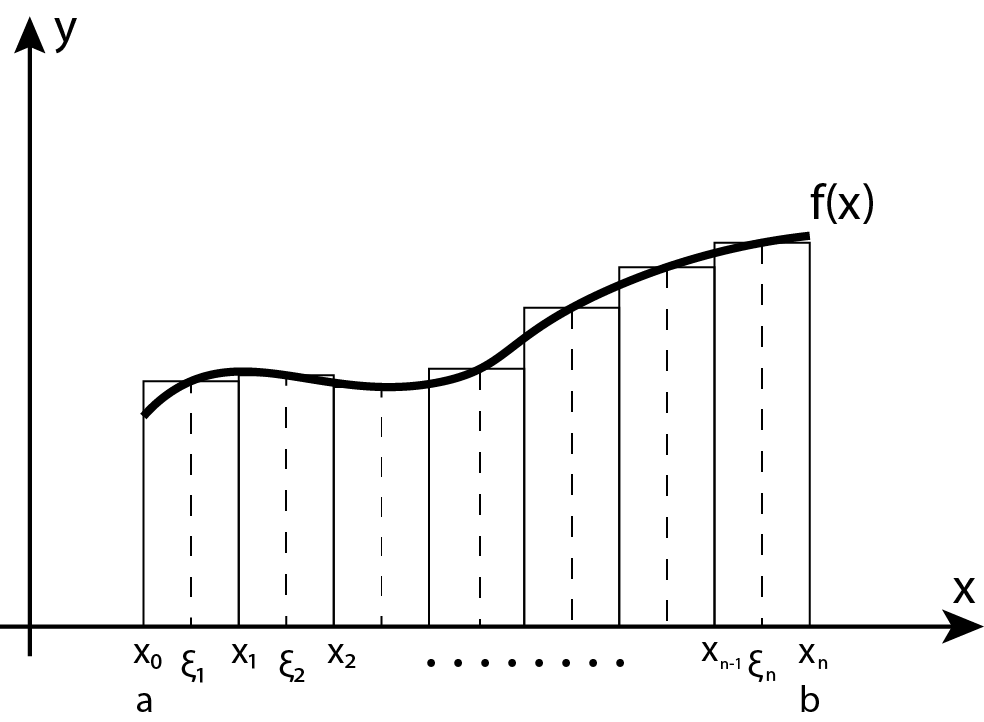
\includegraphics[scale=0.7]{graph1.png}\label{figure1}
    \end{center}
  \end{figure}

  $\Delta i = [x_{i-1}, x_{i}], \quad \Delta x = x_{i} - x_{i-1}$ - длина отрезка $\Delta i$.\\

  Составим сумму $S_{n} = \sum_{i=1}^{n} f(\xi_{i})\Delta x_{i}$, где $f(\xi_{i})$ - высота $i$-го прямоугольника и
  $\Delta x_{i}$ - ширина $i$-го прямоугольника.\\

  $S_{n}$ - площадь ступенчатой фигуры, составленной из прямоугольников под графиком функции $f(x)$.\\

  Говорят, что функция $f$ интегрируема на $[a;b]$, если существует предел интегральных сумм $S_{n}$, то есть
  $\exists \underset{max\Delta x_{i}\rightarrow0}{\lim}S_{n}$, причем этот предел не зависит ни от способа разбиения
  отрезка $[a;b]$, ни от способа выбора точек $\xi_{i}$.\\

  Этот предел называется \textbf{интегралом Римана} функции $f$ на $[a;b]$. Класс интегрируемых функций на отрезке
  $[a;b]$ будем обозначать $R([a;b])$.
\end{definition}

\section{Базы. Предел функции по базе}

\begin{definition}[база множества]
  Пусть $X$ - произвольное множество.\\

  Система $\beta$ подмножеств множества $X$ называется \textbf{базой} на $X$, если:
  \begin{enumerate}
    \item $\forall \beta \in \beta \quad \beta \ne \o$
    \item $\forall \beta_{1}, \beta_{2} \in \beta \ \exists \beta_{3} \in \beta: \quad \beta_{3} \subset \beta_{1}
            \cap \beta_{2}$
  \end{enumerate}
\end{definition}

\begin{example}[баз множества]
  \begin{enumerate}
    \item $\beta = \{X\}$ - база
    \item $X = \mathbb{R}, \quad \beta = \{\beta_{n} = (-\frac{1}{n};\frac{1}{n}), \ n \in \mathbb{N}\}$
    \item $X = \mathbb{R}, \quad \beta = \{\beta_{\epsilon} = \{x: \  0 < |x| < \epsilon\}, \epsilon > 0\}$
          (выколотые окрестности нуля)
  \end{enumerate}
\end{example}

\begin{definition}[предел по базе]
  Пусть $f:X\rightarrow\mathbb{R}, \ \beta$ - база на $X$\\

  Число $A\in\mathbb{R}$ называется \textbf{пределом} функции $f$ \textbf{по базе $\beta$}, если
  $\forall \epsilon > 0 \ \exists$ элемент базы $\beta \in \beta: \quad |f(x) - A| < \epsilon$.
  \begin{equation*}
    \underset{\beta}{\lim} f(x)
  \end{equation*}
\end{definition}

\begin{definition}[предел по базе (МП)]
  Пусть $(Y, d)$ - МП, $f:X\rightarrow Y, \ \beta$ - база на $X$.\\

  $y\in Y$ называется \textbf{пределом} функции $f(x)$ \textbf{по базе $\beta$}, если $\forall \epsilon > 0 \
    \exists \beta \in \beta \ \forall x \in \beta: \quad d(f(x), y) < \epsilon$, или, что то же самое,
  $\forall V_{Y}(y) \ \exists \beta \in \beta \quad f(\beta) \subset V_{Y}(y)$, где $V_{Y}$ - окрестность
  метрического пространства $Y$.
\end{definition}

\begin{theorem}[основные свойства предела по базе]
  Пусть $f:X\rightarrow\mathbb{R}, \ \beta$ - база на $X$:
  \begin{enumerate}
    \item Если $\exists \underset{\beta}{\lim}f(x)$, то $\exists \beta \in \beta: \ f$ ограничена на $\beta$
    \item Если $\underset{\beta}{\lim}f(x) = A$ и $\underset{\beta}{\lim}f(x) = B$, то $A = B$
  \end{enumerate}
\end{theorem}

\clearpage

\begin{theorem}[связь предела по базе с арифметическими операциями]
  Пусть $f:X\rightarrow\mathbb{R}, \ g:X\rightarrow\mathbb{R}, \ \beta$ - база на $X, \quad \underset{\beta}
    {\lim}f(x) = A, \quad \underset{\beta}{\lim}g(x) = B$:
  \begin{enumerate}
    \item $\exists \underset{\beta}{\lim}(f(x)\pm g(x)) = A\pm B$
    \item $\exists \underset{\beta}{\lim}(f(x)g(x)) = AB$
    \item $\exists \underset{\beta}{\lim}(\frac{f(x)}{g(x)}) = \frac{A}{B}$, если $g(x)\ne 0, \ \beta \ne 0$
  \end{enumerate}
\end{theorem}

\begin{theorem}[связь предела функции по базе с неравенствами]
  Пусть $f:X\rightarrow\mathbb{R}, \ g:X\rightarrow\mathbb{R}, \ \beta$ - база на $X$:
  \begin{enumerate}
    \item Если $\exists\beta\in\beta: \quad \forall x \in \beta \ f(x) \leqslant g(x)$, то $\underset{\beta}
            {\lim}f(x) \leqslant \underset{\beta}{\lim}g(x)$
    \item Если $\underset{\beta}{\lim}f(x) < \underset{\beta}{\lim}g(x)$, то $\exists\beta\in\beta \ \forall
            x \in \beta \quad f(x) < g(x)$\\

          Если $\underset{\beta}{\lim}f(x) \geqslant \underset{\beta}{\lim}g(x)$, то $\exists\beta\in\beta \ \forall
            x \in \beta \quad f(x) \geqslant g(x)$
    \item Если $h:X\rightarrow \mathbb{R}$ и $\exists\beta\in\beta: \ \forall x \in \beta \ f(x) \leqslant h(x)
            \leqslant g(x)$ \textbf{И} $A = \underset{\beta}{\lim}f(x) = \underset{\beta}{\lim}g(x)$, то $\underset{\beta}
            {\lim}h(x) = A$
  \end{enumerate}
\end{theorem}

\begin{theorem}[критерий Коши существования предела по базе]
  Существуют две формулировки:
  \begin{enumerate}
    \item Пусть $f:X\rightarrow\mathbb{R}, \ \beta$ - база на $X$.

          Функция $f(x)$ имеет предел по базе $\beta \iff \forall \epsilon > 0 \ \exists\beta\in\beta: \quad \forall
            x_{1},x_{2} \in \beta \ |f(x_{1}) - f(x_{2})| < \epsilon$

    \item Пусть $(Y,d)$ - МП (\textbf{полное}), $f:X\rightarrow Y, \ \beta$ - база на $Y$.

          Функция $f(x)$ имеет предел по базе $\beta \iff \forall \epsilon>0\exists\beta\in\beta: \quad \forall
            x_{1},x_{2} \in \beta \ d(f(x_{1}), f(x_{2})) < \epsilon$
  \end{enumerate}
\end{theorem}

\begin{proof}
  (критерия Коши $\exists$ предела по базе)\\

  $"\rightarrow"$ Пусть $\exists \underset{\beta}{\lim}f(x) = A$. Покажем, что $\forall \epsilon > 0 \exists \beta \in
    \beta: \quad \forall x_{1},x_{2} \in \beta \ |f(x_{1}) - f(x_{2})| < \epsilon$. Рассмотрим $| f(x_{1}) - f(x_{2}) |
    = | f(x_{1} - A) + (A - f(x_{2})) | \leqslant | f(x_{1}) - A | + | f(x_{2}) - A | < \frac{\epsilon}{2} +
    \frac{\epsilon}{2} = \epsilon$.\\

  $"\leftarrow"$ Пусть $\forall \epsilon > 0 \ \exists \beta\in\beta: \quad \forall x_{1},x_{2}\in\beta \ | f(x_{1}) -
    f(x_{2}) |<\epsilon$. Покажем, что $\exists \underset{\beta}{\lim}f(x)$. Возьмем $\beta_{1} \in \beta: \quad
    \forall x_{1},x_{2}\in\beta_{1} \ | f(x_{1}) - f(x_{2}) | < 1$. Возьмем $\beta_{1}'\in\beta: \quad \forall
    x_{1},x_{2}\in\beta_{1}' \ | f(x_{1}) - f(x_{2}) | < \frac{1}{2}$. Пусть $\beta_{2} \subset \beta_{1} \cap \beta_{1}'$
  и так далее.\\

  Таким образом построим систему вложенных множеств: $\beta_{1} \supset \beta_{2} \supset \ldots \supset \beta_{n}
    \supset \ldots$, при этом $\forall x_{1},x_{2} \in \beta_{n} \ | f(x_{1}) - f(x_{2}) | < \frac{1}{2^{n-1}}$.
  Воспользуемся полнотой пространства, то есть в нем $\exists \lim f(x)$, если $f(x)$ - фундаментальная.\\

  $\forall n \in \mathbb{N}$ рассмотрим $x_{n} \in \beta_{n}$. Тогда, если $n < m \ (m \in \mathbb{N})$, то
  для $x_{n} \in \beta_{n}$ и $x_{m} \in \beta_{n} \ | f(x_{n}) - f(x_{m}) | < \frac{1}{2^{n-1}}$.\\

  Таким образом последовательность ${f(x_{n})}$ - фундаментальная $\implies \\ \exists \underset{n\rightarrow\infty}{\lim}
    f(x_{n}) = A$. Покажем, что $A = \underset{\beta}{\lim}f(x)$. Пусть $\epsilon > 0$ задано. Выберем $n\in\mathbb{N}:\quad
    \frac{1}{2^{n-1}} < \frac{\epsilon}{2}$. Возьмем $m>n:\quad | f(x_{m}) - A | < \frac{\epsilon}{2}$. Возьмем $\beta =
    \beta_{n}$. Тогда $\forall x \in \beta \ | f(x) - A | = | f(x) - f(m) + f(x_{m}) - A | \leqslant | f(x) - f(x_{m}) | +
    | f(x_{m}) - A | < \frac{\epsilon}{2} + \frac{\epsilon}{2} = \epsilon$.\\

  Следовательно, $\exists\underset{\beta}{\lim}f(x) = A$.
\end{proof}

\section{Разбиение. Интеграл Римана (v.2)}

\begin{definition}[разбиение]
  Пусть дан отрезок $[a;b]$. \textbf{Разбиением} $P$ отрезка $[a;b]$ называется набор точек $a=x_{0}<x_{1}<\ldots
    <x_{n-1}<x_{n}=b$. То есть $P = \{x_{0},\ldots,x_{n}\}$. Отрезки $[x_{i-1};x_{i}] = \Delta_{i}$.
  $x_{i}-x_{i-1} = \Delta x_{i}$ - длина $i$-го отрезка разбиения $\lambda(P) = \underset{i=\overline{0,n}}
    {\max}\{\Delta x_{i}\}$. Величины $\Delta_{i}, \Delta x_{i}, \lambda(P)$ - параметры ограничения.
\end{definition}

\begin{definition}[разбиение с отмеченными точками]
  \textbf{Разбиением с отмеченными точками} называется пара наборов
  \begin{equation*}
    P(\xi) = \{x_{0},\ldots,x_{n}\},\{\xi_{0},\ldots,\xi_{n}\},
  \end{equation*}
  \center{где $a=x_{0} < \ldots < x_{n}=b, \ \xi_{i}\in [x_{i-1};x_{i}]$.}
  \begin{figure}[h]
    \begin{minipage}[h]{0.49\linewidth}
      \center{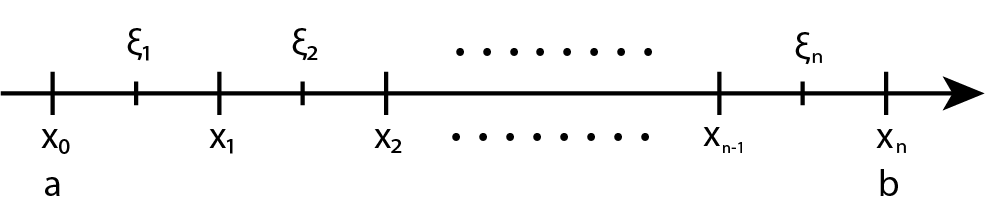
\includegraphics[scale=0.6]{graph2.png}}
    \end{minipage}
    \hfill
    \begin{minipage}[h]{0.49\linewidth}
      Пусть $\Re_{\xi} = \{(P,\xi)\}$ - семейство всевозможных разбиений с отмеченными точками отрезка $[a,b]$.
    \end{minipage}
  \end{figure}
\end{definition}

Рассмотрим $\beta_{\delta} = \{(P,\xi):\quad \lambda(P) < \delta\}, \ \beta_{\delta}\subset P_{\xi}$:

\begin{statement}
  Множество $\beta = \{\beta_{\delta}:\quad \delta > 0\}$ является базой на $\Re_{\xi}$.
\end{statement}

\begin{proof}
  (утверждения 2.3.1.).
  \begin{enumerate}
    \item $\forall\delta>0 \ \beta_{\delta}$ - непусто.\\

          В самом деле, пусть отрезок $[a;b]$ поделен на $n$ равных частей, причем $n$ выбирается из соображений,
          чтобы $\Delta x_{i} = \Delta x \quad \forall i = \overline{1,n} \ (1,\ldots,n), \ \Delta x < \delta$.\\

          Пусть $\xi_{i} \in [x_{i-1};x_{i}]$ - середины отрезков $[x_{i-1};x_{i}]$.

    \item Покажем, что $\forall \beta_{\delta_{1}},\beta_{\delta_{2}} \in \beta \ \exists \beta_{\delta_{3}}
            \subset \beta_{\delta_{1}} \cap \beta_{\delta_{2}}$.\\

          Пусть заданы $\delta_{1}>0, \delta_{2}>0$. Покажем, что $\exists\beta_{3}>0$:\\
          $\beta_{\delta_{3}} \subset \beta_{\delta_{1}} \cap \beta_{\delta_{2}}$. Если $\delta_{1} < \delta_{2}$,
          то $\delta_{3} = \delta_{1}$ или $\delta_{3} = \frac{\delta_{1}}{2}$.
  \end{enumerate}
\end{proof}

\begin{definition}[!]
  Пусть $f:[a;b]\rightarrow\mathbb{R}, \ (P,\xi)$ - разбиение отрезка $[a;b]$ с отмеченными точками. Составим сумму:
  \begin{equation*}
    \sigma(f,(P,\xi)) = \sum_{k=1}^{n}f(\xi_{k})\Delta x_{k}
  \end{equation*}
  Можно смотреть на $\sigma$ для фиксированной функции $f(x)$ как на функцию, сопоставляющую разбиение $(P,\xi)\in
    \Re_{\xi}$ сумме $\sum_{k=1}^{n}f(\xi_{k})\Delta x_{k}$, то есть $\sigma_{f}:\Re_{\xi}\rightarrow\mathbb{R}$
  (то есть $(P,\xi)$ - аргумент функции $\sigma$).\\

  Говорят, что функция $f:[a;b]\rightarrow\mathbb{R}$ интегрируема по Риману на $[a;b]$, если:
  \begin{equation*}
    \exists\underset{\lambda(P)\rightarrow0}{\lim}\sigma_{f}((P,\xi)) = \underset{\lambda(P)\rightarrow0}{\lim}
    \sum_{k=1}^{n}f(\xi_{k})\Delta x_{k}
  \end{equation*}
  Или, что то же самое, если $\forall\epsilon>0 \ \exists\delta>0$ и соответствующий элемент $\beta_{\delta} \in
    \beta:\quad \forall$ разбиения $(P,\xi): \ \lambda(P) < \delta$ выполняется неравенство \\ $| \sigma_{f}
    ((P,\xi)) - I | < 0$:
  \begin{equation*}
    I = \underset{\lambda(P)\rightarrow0}{\lim}\sigma_{f}((P,\xi)) = \int_{a}^{b}f(x)dx
  \end{equation*}
\end{definition}

Обозначим базу $\beta$ из утверждения 2.3.1. как $\lambda(P)\rightarrow0$.

\begin{theorem}[необходимое условие интегрируемости функции]
  $*\_*$

  Если $f:[a;b]\rightarrow\mathbb{R}$ интегрируема на $[a;b]$ (то есть $f\in\mathbb{R}[a;b]$), то \\ $f$
  ограничена на $[a;b]$.
\end{theorem}

\begin{proof}
  От противного:

  Допустим, что $f$ интегрируема на $[a;b]$, но неограничена, то есть: $\forall M>0 \ \exists x \in
    [a;b]: \quad | f(x) | > M$. Покажем, что функция $\sigma ((P,\xi))$ не имеет предела по базе на $[a;b]$.

  То есть $\exists \epsilon > 0: \ \forall \delta > 0 \ \exists (P',\xi')$ и $(P'',\xi''): \quad
    \lambda(P') < \delta, \ \lambda(P'')<\delta \ (\lambda(P'') = \max\Delta x_{i})$, но
  $(\sigma(P'',\xi'') - \sigma(P'',\xi'')) \geqslant \epsilon$.

  Положим, $\epsilon = 1$. Пусть $\delta > 0$ задана. Выберем разбиение с отмеченными точками $(P',\xi')$
  такое, что $\lambda(P')<\delta, \ P' = \{a = x_{0},x_{1},\ldots,x_{n}=b\}, \ \epsilon_{i} \in [x_{1},
    \ldots,x_{n}]$. Поскольку функция $f$ неограничена на $[a;b]$, то существует хотя бы один элемент
  разбиения $[x_{i-1},x_{i}] = \Delta i:$ функция $f$ неограничена на (? Спасибо Максим). В качестве
  $P^{n}$ возьмем $P', \ \xi'' = \{\xi_{1}',\xi_{2}',\ldots,\xi_{i}'',\ldots,\xi_{n}'\}, \
    \lambda(P'')<\delta$ и $|f(\xi_{i}'') - f(\xi_{i}')| > \frac{1}{\Delta x_{i}}$. Разбиения $P'$ и $P''$
  совпадают, точки разбиения так же совпадают, кроме $\xi_{i}''$.

  Рассмотрим $| \sigma((P'',\xi'')) - \sigma((P',\xi')) | = | \sum_{k=1}^{n}\Delta x_{k}f(\xi_{k}') -
    \sum_{k=1}^{n}\Delta x_{k}f(\xi_{k}'') | = | \Delta x_{i}(f(\xi_{i}'') - f(\xi_{i}')) | >
    \frac{\Delta x_{i}}{\Delta x_{i}} = 1 = \epsilon$.
\end{proof}

\section{Критерий интегрируемости}

\subsection{Суммы Дарбу}

\begin{definition}[нижняя/верхняя суммы Дарбу]
  Пусть $f[a;b] \rightarrow \mathbb{R}, \ P$ - произвольное разбиение отрезка $[a;b]$. Числа
  $\underline{S}(P) = \sum_{k=1}^{n}m_{k}\Delta x_{k}$ и $\overline{S}(P) = \sum_{k=1}^{n}M_{k}
    \Delta x_{k}$, где $m_{k} = \underset{\xi \in \Delta k}{\inf}f(\xi), \ M_{k} = \underset{\xi\in\Delta k}
    {\sup}f(\xi)$, называются \textbf{нижней} и \textbf{верхней суммами Дарбу}, отвечающими разбиению $P$.

  \begin{figure}[h]
    \begin{minipage}[h]{0.49\linewidth}
      \center{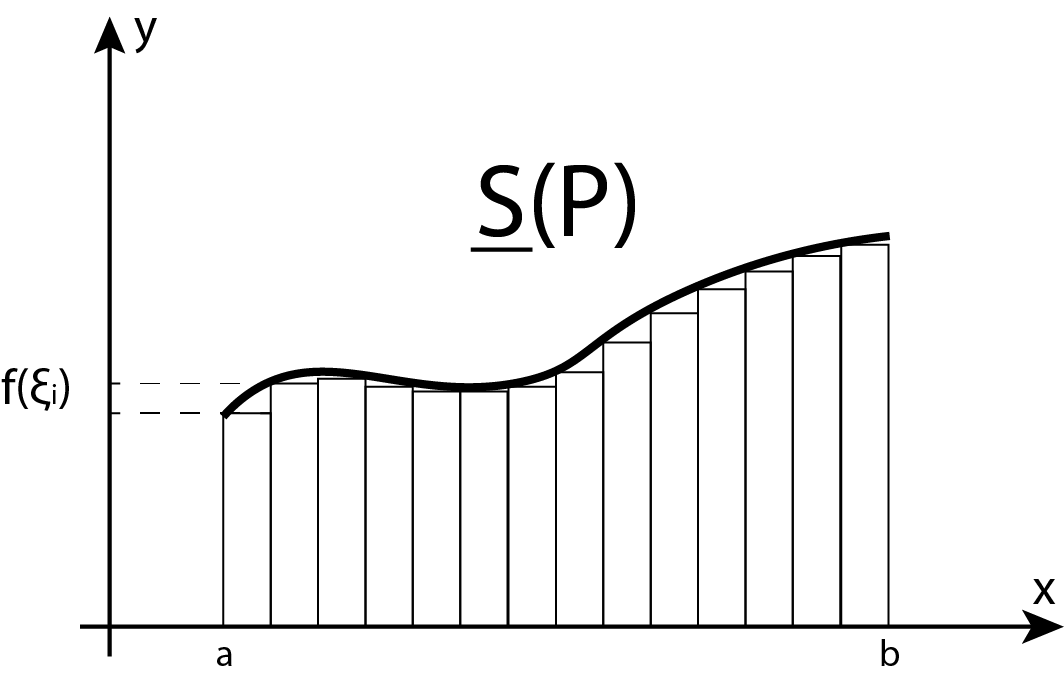
\includegraphics[scale=0.6]{graph4.png}}
    \end{minipage}
    \hfill
    \begin{minipage}[h]{0.49\linewidth}
      \center{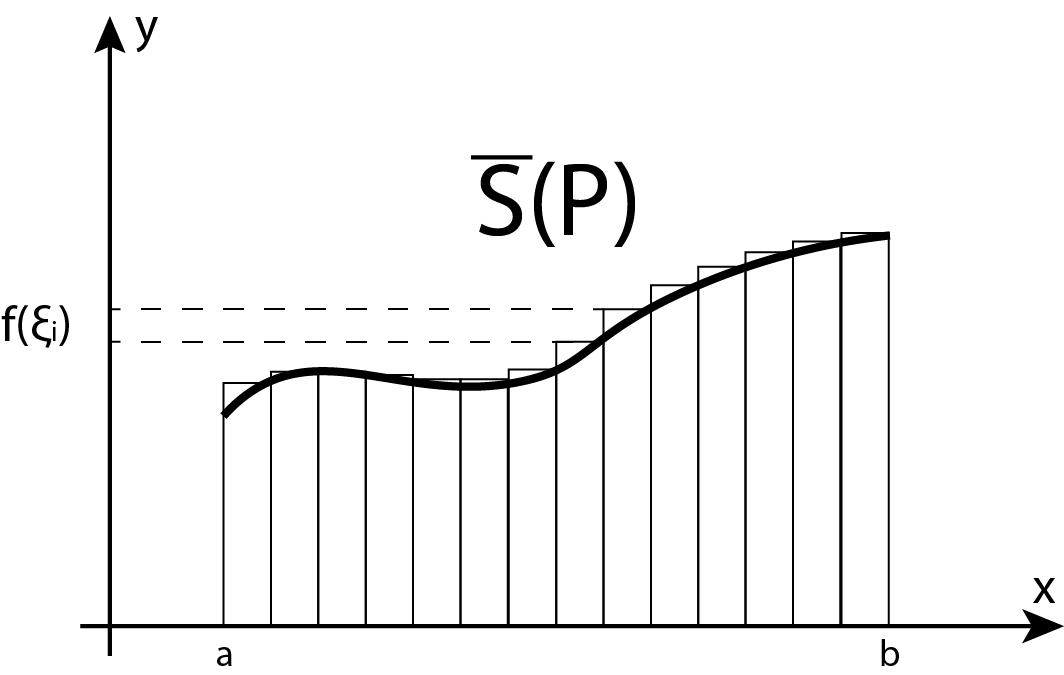
\includegraphics[scale=0.6]{graph3.png}}
    \end{minipage}
  \end{figure}
\end{definition}

\begin{theorem}[свойства сумм Дарбу]
  Свойства:
  \begin{enumerate}
    \item $\forall(P,\xi) \ \underline{S}(P)\leqslant\sigma_{f}((P,\xi))\leqslant\overline{S}(P)$
    \item Если разбиение $P'$ получено из разбиения $P$ добавлением новых точек, то $\underline{S}
            (P') \geqslant \underline{S}(P)$ и $\overline{S}(P')\leqslant\overline{S}(P)$
    \item $\forall P_{1},P_{2} \quad \underline{S}(P_{1})\leqslant\overline{S}(P_{2})$
  \end{enumerate}
\end{theorem}

\begin{proof}
  (теоремы 2.4.1)

  \begin{enumerate}
    \item $\underline{S}(P) = \sum_{k=1}^{n}m_{k}\Delta x_{k} \leqslant \sum_{k=1}^{n}f(\xi_{k})
            \Delta x_{k} \leqslant \sum_{k=1}^{n}M_{k}\Delta x_{k} = \overline{S}(P)$, где $f(\xi_{k}) =
            \sigma((P,\xi))$, вроде
    \item Пусть $P$ - произвольное разбиение отрезка $[a;b]$. Построим $P'$. Добавим на элемент
          разбиения $\Delta i$ новую точку $x'\in [x_{i-1};x_{i}]$.

          Пусть $m_{i}' = \underset{\xi\in[x_{i-1},x_{i}]}{\inf}f(\xi)$ и $m_{i}'' = \underset
            {\xi\in[x_{i}',x_{i}]}{\inf}f(\xi), \ m_{i} = \underset{\xi\in[x_{i-1};x_{i}]}{\inf}f(\xi)$,
          имеем $m_{i}\leqslant m_{i}', \ m_{i} \leqslant m_{i}''$.

          Тогда $\underline{S}(P') - \underline{S}(P) = \sum_{k=1}^{i-1}\Delta x_{k}m_{k} +
            m_{i}' | x' - x_{i-1} | + m_{i}''| x_{i} - x' | + \sum_{k=i+1}^{n}m_{k}\Delta x_{k} - \sum_{k=1}^{n}
            \Delta x_{k}m_{k} = m_{i}'| x' - x_{i-1} | + m_{i}''| x_{i} - x' | - m_{i}\Delta x_{i} \geqslant 0
            \implies \underline{S}(P') \geqslant S(P)$ (вероятно, куча индексов - неправильные).

          Аналогично доказывается для $\overline{S}(P')\leqslant\overline{S}(P)$.
    \item Пусть $P_{1},P_{2}$ - произвольные разбиения отрезка $[a;b]$.

          Возьмем разбиение $P = P_{1}\cap P_{2}$. Тогда, с одной стороны, $P$ получено из $P_{1}$ добавлением
          точек, а с другой стороны - из $P_{2}$ добавлением точек.

          Тогда $\underline{P_{i}} \leqslant \underline{S}(P)$ и $\overline{S}(P_{i})\geqslant S(P)$.

          Тогда верно, что $\underline{S}(P_{2})\leqslant \underline{S}(P)$ и $\overline{S}(P_{2})
            \geqslant \overline{S}(P) \implies \underline{S}(P_{1}) \leqslant \underline{S}(P) \leqslant
            \overline{S}(P)\leqslant \overline{S}(P_{2})$.
  \end{enumerate}
\end{proof}

\begin{effect}
  Множество нижних сумм Дарбу ограничено сверху. Множество верхних сумм Дарбу ограничено снизу.
\end{effect}

\begin{definition}[верхний/нижний интеграл Дарбу]
  Числа $\underline{\mathfrak{I}}=\sup\underline{S}(P)$ и $\overline{\mathfrak{I}}=\inf\overline{S}(P)$ называются
  \textbf{нижним} и \textbf{верхним интегралом Дарбу}.
\end{definition}

Рассмотрим множество разбиений с отмеченными точками отрезка $[a;b] \ \Re = \{(P,\xi)\}$. Построим функцию $\underline{S}:
  \Re_{\xi}\rightarrow\mathbb{R}$ и $\underline{S}((P,\xi)) = \underline{S}(P)$. Аналогично определим $\overline{S}:
  \Re_{\xi}\rightarrow\mathbb{R}$ и $\overline{S}((P,\xi)) = \overline{S}(P)$.

Таким образом сумму Дарбу можно представить как функции на множестве разбиений с отмеченными точками отрезка $[a;b]$.

\begin{theorem}[критерий интегрируемости]
  Функция $f:[a;b]\rightarrow\mathbb{R}$ интегрируема на $[a;b] \iff \underset{\lambda (P)\rightarrow0}{\lim}
    (\overline{S}(P) - \underline{S}(P)) = 0$.
\end{theorem}

\begin{proof}
  (теоремы 2.4.2)

  $"\rightarrow"$ Пусть $f\in\mathbb{R} \ ([a;b])$ (то есть интегрируема на $[a;b]$), то есть $\forall \epsilon > 0 \
    \forall (P,\xi): \ \lambda (P) < \delta \implies | \sigma_{f} ((P,\xi)) - I | < \epsilon$.

  \begin{lemma}
    $\forall P \ \underline{S}(P) = \underset{\xi}{\inf} \sigma_{f}((P,\xi))$ и $\overline{S}(P)=\underset{\xi}{\sup}
      \sigma_{f}((P,\xi))$
  \end{lemma}

  \begin{proof}
    (леммы 2.4.1)

    $\forall P \ \underline{S}(P) \leqslant \sigma_{f}((P,\xi))$.

    Покажем, что $\forall \epsilon > 0 \ \exists \xi = \{\xi_{1},\xi_{2},\ldots,\xi_{n}\}: \ \underline{S}(P) + \epsilon
      > \sigma_{f}(P,\xi)$.

    Выберем $\xi_{1},\xi_{2},\ldots,\xi_{n}: \ f(\xi_{i}) < m_{i} + \frac{\epsilon}{b-a}$.

    Тогда $\sigma_{f}(P,\xi) = \sum_{k=1}^{n}f(\xi_{k})\Delta x_{k} < \sum_{k=1}^{n}(m_{k} + \frac{\epsilon}{b-a})
      \Delta x_{k} = \sum_{k=1}^{n}m_{k}\Delta x_{k} + \frac{\epsilon}{b-a}\sum_{k=1}^{n}\Delta x_{k} = \underline{S}(P)
      + \epsilon \implies \underline{S}(P) = \underset{\xi}{\inf}\sigma_{f}(P,\xi)$.

    Аналогично для $\overline{S}(P) = \underset{\xi}{\sup}\sigma_{f}(P,\xi)$.
  \end{proof}

  $I - \epsilon < \sigma_{f}(P,\xi) < I + \epsilon, \ I - \frac{\epsilon}{2} < \sigma_{f}(P,\xi) < I + \frac
    {\epsilon}{2}$. Из леммы 2.4.1: $\underline{S}(P) + \epsilon > \sigma_{f}(P,\xi) \implies \underline{S}(P) >
    \sigma_{f} (P,\xi) - \epsilon > \sigma_{f}(P,\xi) - \frac{\epsilon}{2} \ (I = \underset{\lambda
      (P)\rightarrow0}{\lim}\sigma_{f}(P,\xi))$

  Рассмотрим $I-\frac{2\epsilon}{3} < I - \frac{\epsilon}{2} \leqslant \underline{S}(P) \leqslant \sigma_{f}(P,\xi)
    \leqslant \overline{S}(P) < \sigma_{f}(P,\xi) + \epsilon < I + \frac{\epsilon}{2} + \epsilon = I + \frac{3\epsilon}{2}
    \ (\overline{S}(P) - \epsilon < \sigma_{f}(P,\xi))$

  Тогда $I - \frac{3\epsilon}{2} < \underline{S}(P) \leqslant \overline{S}(P) < I + \frac{3\epsilon}{2}$, так как
  $\underline{S}(P) \leqslant \overline{S}(P) \implies 0 \leqslant \overline{S}(P) - \underline{S}(P),$

  \begin{center}
    $\overline{S}(P) < I + \frac{3\epsilon}{2}$ \\
    +\\
    $-\underline{S}(P) < -I + \frac{3\epsilon}{2}$
  \end{center}


  $0 \leqslant \overline{S}(P) - \underline{S}(P) < 3\epsilon \implies \underset{\lambda(P)\rightarrow0}{\lim}
    (\overline{S}(P) - \underline{S}(P)) = 0$

  $"\leftarrow"$ Пусть $\underset{\lambda(P)\rightarrow0}{\lim}(\overline{S}(P) - \underline{S}(P)) = 0$.

  Пусть $\epsilon > 0$ задана. Выберем $\delta > 0: \quad 0\leqslant\overline{S}(P) - \underline{S}(P) < \epsilon \
    \forall (P,\xi) : \ d(P) < \delta$.

  Покажем, что $\exists I = \int_{a}^{b} f(x)dx = \underset{\lambda(P)\rightarrow0}{\lim}\sigma_{f}(P,\xi)$.
  Имеем $\overline{S}(P) - \underline{S}(P) < \epsilon$ и $\underline{S}(P) \leqslant I \leqslant \overline{S}(P)$.

  Из неравенств следует, что $\overline{S}(P) < \underline{S}(P) + \epsilon \leqslant I + \epsilon, \
    \underline{S}(P) > \overline{S}(P) - \epsilon \geqslant I - \epsilon$.

  Пусть $(P,\xi)$ - произвольное разбиение: $\lambda(P) < \delta$. Тогда $I - \epsilon < \underline{S}(P)
    \leqslant \sigma_{f}(P,\xi) \leqslant \overline{S}(P) < I + \epsilon \implies I - \epsilon <
    \sigma_{f}(P,\xi) < I + \epsilon \implies | \sigma_{f}(P,\xi) - I | < \epsilon \implies I = \underset
    {\lambda(P)\rightarrow0}{\lim}\sigma_{f}(P,\xi) \implies f\in\mathbb{R} [a;b]$.
\end{proof}

\begin{definition}
  Обозначим $M_{i} - m_{i} = \underset{\xi \in \Delta i}{\sup}f(\xi) - \underset{\xi\in\Delta i}{\inf}f(\xi)
    = \underset{x_{1},x_{2}\in\Delta i}{\sup}| f(x_{1}) - f(x_{2}) | = \omega_{i} = \omega_{i}(f,\Delta i)$.

  $\omega_{i}$ называется \textbf{колебанием} функции $f(x)$ на отрезке $\Delta i$.

  $\overline{S}(P) - \underline{S}(P) = \sum_{i = 1}^{n}\omega_{i}\Delta x_{i}$
\end{definition}

\begin{effect}
  (из критерия интегрируемости)

  $f\in\mathbb{R}[a;b] \iff \underset{\lambda(P)\rightarrow0}{\lim} \sum_{i=1}^{n}\omega_{i}\Delta x_{i} = 0$
\end{effect}

\begin{theorem}[Дарбу]
  Для любой ограниченной функции $f:[a;b]\rightarrow\mathbb{R}$ выполняются равенства:

  \begin{center}
    {\large $\underline{\mathfrak{I}} = \underset{\lambda(P)\rightarrow0}{\lim}\underline{S}(P); \ \overline{\mathfrak{I}}
        = \underset{\lambda(P)\rightarrow0}{\lim}\overline{S}(P)$}
  \end{center}
\end{theorem}

\begin{lemma}
  Пусть $f:[a;b]\rightarrow\mathbb{R}$ ограничена на $[a;b]$, то есть $\exists L > 0: \ \forall x \in [a;b]
    \ | f(x) | < L$. Разбиение $P'$ получено из разбиения $P$ добавлением $m$ точек. Тогда $\overline{S}{P}
    - \overline{S}(P') \leqslant 2L\lambda(P)m$
\end{lemma}

\begin{proof}
  (леммы 2.4.2)

  Пусть $P$ - производное разбиение, $\lambda(P)$.

  Рассмотрим случай, что $P'$ получено добавлением $k$ точек на $i$-тый отрезок разбиения $P$. (график,
  посмотреть у Максима). $\overline{S}(P) - \overline{S}(P') = \sum_{j=1}^{n}M_{j}\Delta x_{j} -
    (\sum_{j=1}^{i-1}M_{j}\Delta x_{j} + \sum_{j = 1}^{k}M_{ij}'\Delta x_{ij} + \sum_{j=i+1}^{n}
    M_{j}\Delta x_{j}) = M_{i}\Delta x_{i} - \sum_{j = 1}^{k}M_{ij}'\Delta x_{ij} = M_{i}\sum_{j=1}^{k}
    \Delta x_{ij} - \sum_{j=1}^{k}M_{ij}'\Delta x_{ij} = \sum_{j=1}^{k}M_{i}\Delta x_{ij} - \sum_{j=1}^{k}
    M_{ij}'\Delta x_{ij} = \sum_{j=1}^{k}(M_{i} - M_{ij}')\Delta x_{ij} \leqslant \sum_{j=1}^{k}2L\Delta x_{ij}
    =$ (вспомним, что $\lambda(P)=\max\{\Delta x_{1},\Delta x_{2},\ldots,\Delta x_{n}\}$) $=2L\sum_{j=1}^{k}
    \Delta x_{ij} = 2L\Delta x_{i} \leqslant 2L\lambda(P)$

  Теперь, если $P'$ получено из $P$ добавлением $m$ точек, то они попадут самое большее на $m$ промежутков.
  Тогда $\overline{S}(P) - \overline{S}(P') \leqslant 2L\lambda (P)m$
\end{proof}

\begin{proof}
  (теоремы 2.4.3, Дарбу)

  $\underline{\mathfrak{I}} \overset{def}{=} \underset{P}{\sup}\underline{S}(P), \ \overline{\mathfrak{I}}
    \overset{def}{=} \underset{p}{\inf}\overline{S}(P)$

  Пусть $\epsilon > 0$ задано. Выберем разбиение $P'$ такое, что $\overline{\mathfrak{I}} + \epsilon >
    \overline{S}(P')$ (**) (определение $\inf$). Положим, что $\delta = \frac{\epsilon}{2Lm}$.

  Пусть $P$ - произвольное разбиение: $\lambda (P) < \delta$.

  Покажем, что $0 \leqslant \overline{S}(P) - \overline{\mathfrak{I}} < \epsilon$.

  Построим разбиение $P'' = P' \cup P$. Тогда $P''$ получено из $P$ добавлением $m$ точек $\implies
    \overline{S}(P) - \overline{S}(P'') \leqslant 2L\lambda(P)m$, где $L>0: \ \forall x \in [a;b] | f(x) |
    < L$. Далее, $\overline{S}(P) - \overline{S}(P'')\leqslant2L\lambda(P)m < 2Lm\delta = \frac{2Lm\epsilon}
    {2Lm} = \frac{\epsilon}{2}$. Кроме того, $P''$ получено из $P'$ добавлением некоторого количества точек.
  \begin{center}
    {\large $\overline{S}(P'')\leqslant\overline{S}(P')\overset{(**)}{<} \overline{\mathfrak{I}} + \frac
        {\epsilon}{2}\implies \overline{S}(P'')-\frac{\epsilon}{2}<\overline{\mathfrak{I}}$}
  \end{center}
  Рассмотрим $0\leqslant\overline{S}(P) - \overline{\mathfrak{I}} < \overline{S}(P) - \overline{S}(P'') +
    \frac{\epsilon}{2} < \frac{\epsilon}{2} + \frac{\epsilon}{2} = \epsilon$
\end{proof}

\subsection{Классы интегрируемых функций}

\begin{theorem}[интегрируемость непрерывных функций]
  Пусть $f:[a;b]\rightarrow\mathbb{R}$ непрерывна на $[a;b]\implies f$ - интегрируема на $[a;b]$
  , то есть $f\in\mathbb{R}[a;b]$.
\end{theorem}

\begin{proof}
  (теоремы 2.4.4)

  Так как $f$ - непрерывна на $[a;b]\implies f$ - равномерно непрерывна на $[a;b]$. Это значит,
  что если $\epsilon>0$ задано, то $\exists\delta>0: \ \forall x_{1},x_{2}\in [a;b]: \
    | x_{1} - x_{2} | < \delta \implies | f(x_{1}) - f(x_{2}) | < \frac{\epsilon}{b - a}$.

  По критерию интегрируемости: $f\in\mathbb{R}[a;b] \iff \underset{\lambda(P)\rightarrow0}{\lim}
    (\overline{S}(P) - \underline{S}(P)) = 0 \ \forall (P;\xi)$ - разбиение.

  $\overline{S}(P) - \underline{S}(P) = \sum\omega_{i}\Delta x_{i}$, где $\omega_{i} = \underset
    {x_{1},x_{2}\in\Delta i}{\sup} | f(x_{1}) - f(x_{2}) |$.

  $\overline{S}(P) = \sum M_{i}\Delta x_{i}, \ M_{i} = \underset{\xi\in\Delta x_{i}}{\sup}f(\xi)$.

  $\omega_{i} = M_{i} - m_{i} = \underset{\xi\in\Delta i}{\sup}f(\xi) - \underset{\xi\in\Delta i}
    {\inf}f(\xi) = \underset{x_{1},x_{2}\in\Delta i}{\sup}| f(x_{1}) - f(x_{2}) |$.

  $\overline{S}(P) - \underline{S}(P) = \sum M_{i}\Delta x_{i} - \sum m_{i}\Delta x_{i} =
    \sum \omega_{i}\Delta x_{i}$.

  Таким образом критерий интегрируемости: $f$ - интегрируема на $[a;b] \iff \underset{\lambda
      (P)\rightarrow0}{\lim}\sum\omega_{i}\Delta x_{i} = 0$, то есть $\forall \epsilon > 0 \
    \exists \delta > 0: \ \forall (P;\xi): \ \lambda(P)<\delta\implies 0 \leqslant\sum\omega_{i}
    \Delta x_{i} < \epsilon$.

  Пусть $\epsilon > 0$ задано. Возьмем $(P;\xi)$ - разбиение такое, что $\lambda(P) < \delta$.
  Тогда $\sum\omega_{i}\Delta x_{i} = \sum \underset{x_{1},x_{2}\in\Delta i}{\sup}
    | f(x_{1}) - f(x_{2}) |\Delta x_{i}\leqslant \sum \frac{\epsilon}{b - a} \Delta x_{i} =
    \frac{\epsilon}{b - a}\sum \Delta x_{i} = \frac{\epsilon}{b - a}(b-a) = \epsilon$
\end{proof}

\begin{theorem}[интегрируемость функций с конечным числом точек разрыва]
  Пусть $f:[a;b]\rightarrow\mathbb{R}$ - ограничена и имеет на $[a;b]$ конечное число точек
  разрыва. Тогда $f\in\mathbb{R}[a;b]$ интегрируема на $[a;b]$.
\end{theorem}

\begin{proof}
  (теоремы 2.4.5)

  Пусть $L > 0: \ \forall x \in [a;b] \ | f(x) | < L$ (ограничена). Пусть $f$ имеет $k$ точек
  разрыва на $[a;b]$.

  Пусть $\epsilon > 0$ задано. Возьмем $\delta_{1} = \frac{\epsilon}{16Lk}$. Для каждой точки
  разрыва построим $\delta_{1}$-окрестность.

  Пусть $U$ - множество таких окрестностей. $U$ - открытое множество. Рассмотрим
  $V = [a;b]\setminus U \implies V$ - замкнутое (так как его дополнение открытое). Из того,
  что $V$ - ограничено и замкнуто $\implies V$ - компактное. Функция $f$ - непрерывна на $V
    \implies$ из того, что $V$ - компактно и $f$ - непрерывна на $V \implies f$ - равномерно
  непрерывна на $V\implies \forall\epsilon>0 \ \exists\delta_{2}>0: \ \forall x_{1},x_{2}\in V:
    \ | f(x_{1}) - f(x_{2}) | < \frac{\epsilon}{2(b-a)}$.

  Положим, что $\delta = \min\{\delta_{1},\delta_{2}\}$. Пусть $P$ - произвольное разбиение
  отрезка $[a;b]: \ \lambda(P) < \delta$.

  Рассмотрим $\sum \omega_{i}\Delta x_{i} =  \sum'\omega_{i}\Delta x_{i} + \sum''\omega_{i}
    \Delta x_{i} \leqslant | \sum'$ берется по всепм отрезкам разбиения, $k$-тые пересекаются
  с $U$, $\sum''$ - по всем остальным $| \leqslant \sum'\omega_{i}\Delta x_{i} + \sum''
    \frac{\epsilon}{2(b-a)}\Delta x_{i} \leqslant 2L2\delta_{1}k + \frac{\epsilon}{2(b-a)}\sum''
    \Delta x_{i} < \frac{4Lk\epsilon}{8Lk} + \frac{\epsilon}{2(b-a)}(b-a) = \frac{\epsilon}{2}
    + \frac{\epsilon}{2} = \epsilon$.

  Дополнение: $(\overline{S}(P) - \overline{S}(P') \leqslant
    2L\lambda(P)m, \ \sum M_{i}\Delta x_{i} - \sum M_{i}' \Delta x_{i})$.
  $\sum'\omega_{i}\Delta x_{i} = \sum\underset{x_{1},x_{2}\in\Delta i \cap k}{\sup}
    | f(x_{1}) - f(x_{2}) |\Delta x_{i} \leqslant 2L2\delta_{1}k$

\end{proof}

{\Large ГРАФИКИ НАДО НАРИСОВАТЬ}

\begin{theorem}[интегрируемость монотонных функций]
  Пусть $f:[a;b]\rightarrow\mathbb{R}$ - монотонна на $[a;b]\implies f$ - интегрируема на $[a;b]$.
\end{theorem}

\begin{proof}
  (теоремы 2.4.6)

  Пусть $f$ - не убывает на $[a;b]$. Пусть $\epsilon>0$ задано. Возьмем $\delta = \frac{\epsilon}
    {f(b) - f(a)}$. Тогда, если $P$ - произвольное разбиение $[a;b]: \ \lambda(P)<\delta$, то
  $\sum\omega_{i}\Delta x_{i} \overset{monoton.}{=} \sum (f(x_{i}) - f(x_{i-1}))\Delta x_{i} <
    \delta \sum (f(x_{i}) - f(x_{i-1})) = \delta (f(b) - f(a)) = \epsilon$.
\end{proof}

\subsection{Свойства интегрируемых функций}

\begin{theorem}
  Пусть $f\in\mathbb{R}[a;b], \ g\in\mathbb{R}[a;b]$. Тогда:
  \begin{enumerate}
    \item $f\pm g \in R[a;b]$.
    \item $\alpha f \in R[a;b], \ \alpha \in \mathbb{R}$.
    \item $f*g\in R[a;b]$.
    \item $|f|\in R[a;b]$, при этом:
          \begin{itemize}
            \item $\int_{a}^{b}(f\pm g)dx = \int_{a}^{b}f(x)dx \pm \int_{a}^{b}g(x)dx$
            \item $\int_{a}^{b}\alpha f(x)dx = \alpha \int_{a}^{b}f(x)dx$
            \item $|\int_{a}^{b}f(x)dx | \leqslant \int_{a}^{b}|f(x)|dx$
          \end{itemize}
  \end{enumerate}
\end{theorem}

\begin{proof}
  (теоремы 2.4.7)

  \begin{enumerate}
    \item $\int_{a}^{b}(f(x)\pm g(x))dx = \underset{\lambda(P)\rightarrow0}{\lim}\sum(f(\xi_{i})
            \pm g(\xi_{i}))\Delta x_{i} = \underset{\lambda(P)\rightarrow0}{\lim}\sum f(\xi_{i})\Delta
            x_{i} = \int_{a}^{b}f(x)dx + \int_{a}^{b}g(x)dx$.
    \item Аналогично.
    \item Покажем, что если $f\in R[a;b]$, то $f^{2}\in R[a;b]$. Рассмотрим $| f^{2}(x_{1}) -
            f^{2}(x_{2}) | = | (f(x_{1}) - f(x_{2}))(f(x_{1}) - f(x_{2})) | \leqslant | f(x_{1}) -
            f(x_{2}) |(|f(x_{2})| + | f(x_{2}) |) < 2L| f(x_{1}) - f(x_{2}) |$, где $L>0: \ \forall x
            \in [a;b] \ | f(x) | < L$ (интегрируема $\implies$ ограничена).

          Пусть $P$ - произвольное разбиение. Пусть $\epsilon > 0$ задано. Возьмем $\delta>0$ и
          $P: \ \lambda(P) < \delta \quad \omega_{i}(f^{2},\Delta_{i}) \leqslant 2L\omega_{i}
            (f,\Delta_{i})$.\\

          $\underset{i}{\sum}w_{i}(f^{2},\Delta_{i})\Delta x_{i} \leqslant (\underset{i}{\sum}\omega_{i}(f,
              \Delta_{i})\Delta_{i})2L$.\\

          Так как $f\in R[a;b]$, то $\underset{i}{\sum}\omega_{i}(f,\Delta_{i})\Delta x_{i}\rightarrow 0
            \implies$ по лемме о двух миллиционерах, $\underset{i}{\sum}\omega_{i}(f^{2},\Delta_{i})\Delta
            x_{i}\rightarrow0 \implies$ (по критерию интегрируемости) $f^{2}\in R[a;b]$.\\

          $fg = \frac{1}{4}((f+g)^{2}-(f-g)^{2})\implies fg \in R[a;b]$.
    \item Рассмотрим $||f(x_{1})| - | f(x_{2}) || \leqslant | f(x_{1}) - f(x_{2}) |, \ x_{1},x_{2}\in
            \Delta_{i} \implies \omega_{i}(|f|,\Delta_{i})\leqslant \omega_{i}(f,\Delta_{i})$. \\

          $0 \leqslant \underset{i}{\sum}\omega_{i}(| f |,\Delta_{i})\Delta x_{i} \leqslant \underset{i}{\sum}
            \omega_{i}(f,\Delta_{i})\Delta x_{i} \implies |f|\in R[a;b].$

          Рассмотрим $| \underset{i}{\sum}f(\xi_{i}) | \leqslant \underset{i}{\sum} | f(\xi_{i}) |\Delta x_{i}
            \implies \underset{\lambda(P)\rightarrow 0}{\lim}| \underset{i}{\sum}f(\xi_{i})\Delta x_{i} |
            \leqslant \underset{\lambda(P)\rightarrow0}{\lim}\underset{i}{\sum} | f(\xi_{i}) |\Delta x_{i}, \quad
            | \int_{a}^{b}f(x)dx | \leqslant \int_{a}^{b} |f(x)|dx$.
  \end{enumerate}
\end{proof}

\subsection{Аддитивность интеграла Римана}

\begin{definition}
  Пусть $a>b, \ a,b\in\mathbb{R}$, положим $\int_{a}^{b}f(x)dx = -\int_{b}^{a}f(x)dx$. Если $a=b$, то
  $\int_{a}^{a=b}f(x)dx =0$.
\end{definition}

\begin{theorem}[Аддитивность интеграла Римана]
  Пусть даны точки $a,b,c\in \mathbb{R}$. Если $f$ - интегрируема на большем из отрезков $[a;b],\ [a,c],\
    [b,c]$, то $f$ - интегрируема и на меньших отрезках. И наоборот, если $f$ интегрирема на двух меньших отрезках,
  то она интегрируема и на большем отрезке. При этом:
  \begin{equation*}
    \int_{a}^{b}f(x) dx + \int_{b}^{c}f(x)dx + \int_{c}^{a}f(x)dx = 0
  \end{equation*}
\end{theorem}

\begin{proof}[теоремы 2.4.8]
  Пусть $a<b<c$.

  Построим такое разбиение отрезка $[a;c]$ с отмеченнымыми точками, что точка $b$ будет его точкой разбиения
  $P = {x_{0}, x_{1}, \ldots, b, \ldots, x_{n}}$.

  Тогда $\underset{P}{\sum}f(\xi_{i})\Delta x_{i} < \underset{P'}{\sum}f(\xi_{i})\Delta x_{i} +
    \underset{P''}{\sum}f(\xi_{i})\Delta x_{i}$, где $P'$ - разбиение отрезка левеее точки $b$, $P''$ - правее
  точки $b$.

  Покажем, что если $f\in R[a;c]$, то $f\in R[a;b]$. В самом деле, $\underset{P'}{\sum}\omega_{i}\Delta x_{i}
    \leqslant \underset{P}{\sum}\omega_{i}\Delta x_{i}\rightarrow 0 \implies f\in R[a;b]$. Аналогично, можно
  показать, что $f\in R[b;c]$. Если $f$ - интегрируема на $[a;b]$ и $f\in R[b;c] \implies \underset{P'}{\sum}
    \omega_{i}\Delta x_{i} \rightarrow0, \ \underset{P''}{\sum}\omega_{i}\Delta x_{i} \rightarrow0 \implies$
  учитывая то, что $\underset{P}{\sum}f(\xi_{i})\Delta x_{i} < \underset{P'}{\sum}f(\xi_{i})\Delta x_{i} +
    \underset{P''}{\sum}f(\xi_{i})\Delta x_{i}$, тогда $\underset{P}{\sum}\omega_{i}\Delta x_{i}\rightarrow0
    \implies f\in R[a;c]$, а так же то, что $\int_{a}^{c}f(x) dx \ \int_{a}^{b}f(x) dx + \int_{b}^{c}f(x)dx$.
\end{proof}

\subsection{Монотонность интеграла Римана}

\begin{theorem}
  Если $a<b$ и $f\in R[a;b]$ и:
  \begin{enumerate}
    \item $\forall x \in [a;b] \ f(x) \geqslant 0$, то $\int_{a}^{b} f(x) dx \geqslant 0$
    \item $\forall x \in [a;b] \ f(x) > 0$, то $\int_{a}^{b}f(x)dx > 0$
  \end{enumerate}
\end{theorem}

\begin{proof}
  (теоремы 2.4.9)

  \begin{enumerate}
    \item Почти очевидно (по определению интеграла Римана и свойствам предела)
    \item Пусть $\forall x \in [a;b] f(x) > 0$. Покажем, что $\int_{a}^{b} f(x) dx > 0$. Допустим, что
          $\int_{a}^{b}f(x) dx = 0$. Тогда $\underset{\lambda(P)\rightarrow0}{\lim}\overline{S}(P)=0$.

          Тогда можно взять такое разбинеие $P: \ \overline{S}(P) < \frac{b-a}{2}$. Тогда у этого разбиения $P
            \exists$ отрезок $\Delta_{i}: \ M_{i} = \underset{x \in \Delta_{i}}{\sup}f(x) < \frac{1}{2}$. В самом деле,
          если $M_{i} \geqslant \frac{1}{2} \ \forall i$, то $\overline{S}(P) = \underset{i}{\sum}M_{i}\Delta x_{i}
            \geqslant \frac{1}{2}\underset{i}{\sum}\Delta x_{i} = \frac{b-a}{2}$, противоречие с выбраным $P$.

          Обозначим $\Delta_{i} = [a_{1},b_{1}]$. Так как $f\in R[a;b] \implies f\in R[a_{1},b_{1}]$. При этом
          $\int_{a}^{b}f(x)dx = 0$. Пусть $P_{1}$ - разбиение отрезка $[a_{1},b_{1}]: \ \overline{S}(P_{1}) <
            \frac{b_{1} - a_{1}}{4} \implies \exists$ отрезок разбиения $[a_{2},b_{2}] \subset [a_{1},b_{1}]: \
            \underset{x\in [a_{2},b_{2}]}{\sup}f(x) < \frac{1}{4}$ и так далее.

          Таким образом получим систему вложенных отрезков $[a;b] \supset [a_{1},b_{1}] \supset [a_{2},b_{2}] \supset
            \ldots$, при этом $\underset{x\in[a_{k},b_{k}]}{\sup}f(x) < \frac{1}{2^{k}}$. Пусть $c \in \underset
            {k=1}{\overset{\infty}{\cap}}[a_{k};b_{k}]$. Тогда $f(c) > 0$. С другой стороны, $f(c) < \frac{1}{2^{k}}
            \implies f(c) = 0$ - противоречие $\implies \int_{a}^{b}f(x)dx > 0$.
  \end{enumerate}
\end{proof}

\begin{effect}
  (теоремы 2.4.9)
  \begin{enumerate}
    \item Если $a<b, \ f,g \in R[a;b]$ и:
          \begin{enumerate}
            \item $\forall x \in [a;b] \ f(x) \leqslant g(x)$, то $\int_{a}^{b}f(x) dx \leqslant
                    \int_{a}^{b}g(x)dx$
            \item $\forall x \in [a;b] \ f(x) < g(x)$, то $\int_{a}^{b}f(x)dx < \int_{a}^{b}g(x) dx$
                  \begin{proof}
                    Очевидно, $g(x) - f(x) \geqslant 0$.
                  \end{proof}
          \end{enumerate}
    \item Если $f\in R[a;b], \ a<b, \ M = \underset{x \in [a;b]}{\sup}f(x), \ m = \underset{x\in[a;b]}
            {\inf}f(x)$, то $m(b-a) \leqslant \int_{a}^{b}f(x)dx \leqslant M(b-a)$.
          \begin{proof}
            $\forall$ разбиения $P$ с отмеченными точками верно: $\underset{i}{\sum}m\Delta x_{i} \leqslant
              \underset{i}{\sum}f(\xi_{i})\Delta x_{i} \leqslant \underset{i}{\sum} M\Delta x_{i}$ и
            $m(b-a) \leqslant \underset{i}{\sum}f(\xi_{i})\Delta x_{i} \leqslant M(b-a)$.

            Переходя к пределу получаем то, что нужно было доказать.
          \end{proof}
    \item (Теорема о среднем)

          Пусть $f\in R[a;b] (a>b, a<b), \ m = \underset{x \in[a;b]}{\inf}f(x), \ M = \underset{x \in[a;b]}{\sup}f(x)$.
          Тогда существует $\mu \in [m;M]: \ \int_{a}^{b}f(x)dx = \mu (b-a)$.

          \begin{proof}
            Пусть $a<b$. Тогда (из 2-го пункта) $m(b-a) \leqslant \int_{a}^{b}f(x)dx\leqslant M(b-a), \ (b-a>0)$.

            $m \leqslant \frac{1}{b-a}\int_{a}^{b}f(x)dx \leqslant M$. Пусть $\mu \ \frac{1}{b-a} \frac{1}{b-a}
              \int_{a}^{b}f(x) dx \implies \frac{a}{b}f(x)dx = \mu(b-a)$. Если $a > b$, то $m(a-b) \leqslant
              \int_{a}^{b}f(x)dx \leqslant M(a-b)$ (домножим на $-1$), $m(b-a)\geqslant \int_{a}^{b}f(x)dx \geqslant
              M(b-a)\implies m \leqslant \frac{1}{b-a}\int_{a}^{b}f(x) dx \leqslant M$.
          \end{proof}

          \begin{effect}
            Если, кроме того, $f(x)$ - непрерывна на $[a;b]$, то $\exists c \in [a;b]: \ \int_{a}^{b}f(x)dx =
              f(x)(b-a)$.
          \end{effect}
          \begin{proof}
            Доказательство следует из теоремы Больцано-Коши о промежуточном значении.
          \end{proof}
  \end{enumerate}
\end{effect}

\begin{theorem}[Первая теорема о среднем]
  Пусть $f,g\in R[a;b] (a>b, a<b), \ m = \underset{x\in[a;b]}{\inf}f(x), \ M = \underset{x\in[a;b]}{\sup}f(x)$
  и $g$ не меняет свой знак на $[a;b]$. Тогда $\exists \mu \in [m;M]: \ \int_{a}^{b}f(x)g(x)dx = \mu \int_{a}^{b}
    g(x)dx$.
\end{theorem}

\begin{proof}
  Пусть $a<b$ и $\forall x \in [a;b] \ g(x) \geqslant 0$. Имеем, что $m\leqslant f(x) \leqslant M, \ (g(x) > 0), \
    mg(x) \leqslant f(x)g(x) \leqslant Mg(x) \implies m \int_{a}^{b}g(x)dx \leqslant \int_{a}^{b}f(x)g(x)dx
    \leqslant M\int_{a}^{b}g(x)dx$. Если $\int_{a}^{b}g(x)dx = 0 \implies \int_{a}^{b}f(x)g(x)dx = 0 \implies
    \int_{a}^{b}f(x)g(x)dx = \mu \int_{a}^{b}g(x)dx$. Если $\int_{a}^{b}g(x)dx \ne 0$, то поделим в неравенстве
  $m \int_{a}^{b}g(x)dx \leqslant \int_{a}^{b}f(x)g(x)dx \leqslant M\int_{a}^{b}g(x)dx$ все на $\int_{a}^{b}
    g(x)dx > 0: \quad m \leqslant \frac{\int_{a}^{b}f(x)g(x)dx}{\int_{a}^{b}g(x)dx} \leqslant M$, где
  $\frac{\int_{a}^{b}f(x)g(x)dx}{\int_{a}^{b}g(x)dx} = \mu$.

  Аналогично доказываются остальные случаи $(a<b, \ g(x) \leqslant 0; \ a>b, \ g(x)\geqslant 0)$.
\end{proof}

\section{Интеграл Римана как функция верхнего предела интегрирования}

\begin{definition}
  Пусть $f\in R[a;b], \ x \in [a;b]$.

  Рассмотрим функцию $F(x) = \int_{a}^{x}f(t)dt, \ F(x)$ определена для $\forall x \in [a;b]$.
\end{definition}

\begin{theorem}[непрерывность интеграла Римана]
  Если $f\in R[a;b]$, то $F(x) = \int_{a}^{x}f(t)dt$ - непрерывна на $[a;b]$.
\end{theorem}

\begin{proof}
  Пусть $h\in \mathbb{R}: \ x + h \in [a;b]$. Тогда $F(x+h) = \int_{a}^{x+h}f(t)dt$. Пусть
  $\epsilon>0$ задано. Покажем, что $\exists\delta>0: \ \forall h \in \mathbb{R}: \ |h|<\delta \
    | F(x+h) - F(x) | < \epsilon$.

  Рассмотрим $| F(x+h) - F(x) | = | \int_{a}^{x+h}f(t)dt - \int_{a}^{x}f(t)dt | = | \int_{a}^{x}f(t)dt +
    \int_{x}^{x+h}f(t)dt - \int_{a}^{x}f(t)dt | = | \int_{x}^{x+h}f(t)dt | \leqslant |\int_{x}^{x+h}| f(t) |dt|$.
  Так как $f\in R[a;b]$, то $f$ - ограничена на $[a;b]$, то есть $\exists L > 0: \ \forall x \in [a;b] \
    | f(x) | \leqslant L$. Тогда $|\int_{x}^{x+h}| f(t) |dt| \leqslant | L \int_{x}^{x+h}dt |$, так как
  \begin{equation*}
    \int_{x}^{x+h}1dt = \underset{\lambda(P)\rightarrow0}{\lim}\sum_{i=1}^{n}1\Delta x_{i} = | h |,
  \end{equation*}
  тогда $\delta = \frac{\epsilon}{L}$, что и требовалось доказать.
\end{proof}

\begin{theorem}[о дифференцируемости интеграла Римана как функции по верхнему пределу]
  Пусть $f\in R[a;b], \ x \in [a;b]$ и $f$ непрерывна в точке $x$, тогда функция $F(x) = \int_{a}^{x}f(t)dt$
  дифференцируема в точке $x$, причем:
  \begin{equation*}
    F'(x) = f(x) \implies (\int_{a}^{x}f(t)dt)_{x}'=f(x)
  \end{equation*}
\end{theorem}

\begin{proof}
  Пусть $h\in\mathbb{R}: \ x+h \in [a;b]$.

  Рассмотрим $|\frac{F(x+h) - F(x)}{h} - f(x)| = | \frac{1}{h}(\int_{a}^{x+h}f(t)dt - \int_{a}^{x}f(t)dt) -
    f(x) | = | \frac{1}{h} \int_{a}^{x+h}f(t)dt - f(x) | = | \frac{1}{h}\int_{x}^{x+h}f(t)dt - \frac{f(x)}{h}
    \int_{x}^{x+h}dt | = | \frac{1}{h}(\int_{x}^{x+h}f(t)dt - \int_{x}^{x+h}f(x)dt) | = | \frac{1}{h}
    (\int_{x}^{x+h}(f(t)-f(x))dt) | = \frac{1}{|h|}| \int_{x}^{x+h}| f(t) - f(x) |dt |$.

  Так как $f$ - непрерывна в точке $x$, то $\forall \epsilon>0 \ \exists \delta>0: \ \forall h: \ |h|<\delta
    \ | f(t) - f(x) | < \epsilon$, где $t\in[x;x+h]$.

  Тогда $|\frac{F(x+h) - F(x)}{h} - f(x) | \leqslant \frac{1}{|h|}| \int_{x}^{x+h}| f(t) - f(x) |dt | <
    \frac{1}{|h|}\epsilon| \int_{x}^{x+h}dt | = \frac{1}{|h|}\epsilon|h| = \epsilon$

  Таким образом, по определению производной:
  \begin{equation*}
    \underset{h\rightarrow0}{\lim}\frac{F(x+h) - F(x)}{h} = f(x) = F'(x).
  \end{equation*}
\end{proof}

\begin{effect}
  Если $f$ - непрерывна на $[a;b]$, то на $[a;b]$ она имеет первообразную, которая равна:
  \begin{equation*}
    \Phi (x) = \int_{a}^{x}f(t)dt + C
  \end{equation*}
\end{effect}

\begin{remark}
  Рассмотрим следующие классы (множества/пространства) функций:
  \begin{itemize}
    \item $R[a;b]$ - множество интегрируемых на $[a;b]$ функций;
    \item $C[a;b]$ - множество непрерывных на $[a;b]$ функций;
    \item $C^{o}[a;b]$ - множество дифференцируемых на $[a;b]$ функций.
  \end{itemize}
  Получаем:
  \begin{equation*}
    C^{o}[a;b]\subset C[a;b] \subset R[a;b].
  \end{equation*}
\end{remark}

\begin{theorem}[вторая теорема о среднем]
  Пусть $f,g\in R[a;b]$, причем $f$ - монотонна на $[a;b]$. Тогда $\exists \xi \in [a;b]:$
  \begin{equation*}
    \int_{a}^{b}f(x)g(x)dx = f(a)\int_{a}^{\xi}g(x)dx + f(b)\int_{\xi}^{b}g(x)dx
  \end{equation*}
\end{theorem}

\begin{lemma}
  Пусть $f,g\in R[a;b]$, причем $f$ - невозрастающая и неотрицательная.

  Тогда $\exists \xi \in [a;b]:$
  \begin{equation*}
    \int_{a}^{b}f(x)g(x)dx = f(a)\int_{a}^{\xi}g(x)dx.
  \end{equation*}
\end{lemma}

\begin{proof}
  (леммы)

  Пусть $P$ - произвольное разбиение отрезка $[a;b]: \ a = x_{0} < x_{1} < \ldots < x_{n-1} < x_{n} = b$.
  Тогда $\int_{a}^{b}f(x)g(x)dt = \sum_{i=1}^{n}\int_{x_{i-1}}^{x_{i}}f(x)g(x)dx \\ + \sum_{i=1}^{n}
    \int_{x_{i-1}}^{x_{i}}f(x_{i-1})g(x)dx - \sum_{i=1}^{n}\int_{x_{i-1}}^{x_{i}}f(x_{i-1})g(x)dx =
    \sum_{i=1}^{n}\int_{x_{i-1}}^{x_{i}}(f(x)-f(x_{i-1}))g(x)dx + \sum_{i=1}^{n}\int_{x_{i-1}}^{x_{i}}
    f(x_{i-1})g(x)dx =$ (где $\sum_{i=1}^{n}\int_{x_{i-1}}^{x_{i}}(f(x)-f(x_{i-1}))g(x)dx = \rho$ и
  $\sum_{i=1}^{n}\int_{x_{i-1}}^{x_{i}}f(x_{i-1})g(x)dx = \sigma$) $= \rho + \sigma$.

  Устремим $\lambda(P)\rightarrow0$:
  \begin{equation*}
    \int_{a}^{b}f(x)g(x)dx = \underset{\lambda(P)\rightarrow0}{\lim}\rho + \underset{\lambda(P)\rightarrow0}
    {\lim}\sigma
  \end{equation*}
  Покажем, что пределы существуют, более того: $\underset{\lambda(P)\rightarrow0}{\lim}\rho = 0$.

  Так как $g(x)\in R[a;b] \implies g$ - ограничена на $[a;b]$, то есть $\exists L > 0: \ \forall x
    \in [a;b] \ | g(x) |\leqslant L$.

  Рассмотрим $\omega_{i} = \omega_{i}(f,\Delta_{i}) = \underset{\xi_{1},\xi_{2}=\Delta_{i}}{\sup}
    | f(\xi_{1}) - f(\xi_{2}) |$. Так как $f\in R[a;b]$, то по критерию интегрируемости:
  $\underset{i}{\sum}\omega_{i}\Delta x_{i} \rightarrow 0$.

  Тогда $| \rho | = | \sum_{i=1}^{n} \int_{x_{i-1}}^{x_{i}}(f(x) - f(x_{i-1}))g(x)dx |\leqslant
    \sum_{i=1}^{n}\int_{x_{i-1}}^{x_{i}}| f(x) - f(x_{i-1}) | | g(x) |dx \leqslant\sum_{i=1}^{n}
    \int_{x_{i-1}}^{x_{i}}\omega_{i}Ldx = L\sum_{i=1}^{n}\omega_{i}\int_{x_{i-1}}^{x_{i}}dx =
    L\sum_{i=1}^{n}\omega_{i}\Delta x_{i}$.

  Пусть $\epsilon > 0$ задано. Выберем $\delta>0: \ \forall P: \ \lambda(P) < \delta$ и
  $\sum_{i=1}^{n}\omega_{i}\Delta x_{i} < \frac{\epsilon}{L}$.

  Имеем, что $|\rho| \leqslant L\sum_{i=1}^{n}\omega_{i}\Delta x_{i} < L\frac{\epsilon}{L} =
    \epsilon \implies \underset{\lambda(P)\rightarrow0}{\lim}\rho = 0$.

  Тогда $\int_{a}^{b}f(x)g(x)dx = \underset{\lambda(P)\rightarrow0}{\lim}\sum_{i=1}^{n}
    \int_{x_{i-1}}^{x_{i}}f(x_{i-1})g(x)dx$. $\underset{\lambda(P)\rightarrow0}{\lim}\sigma$
  существует, так как $\int_{a}^{b}f(x)g(x)dx = const$ и $\underset{\lambda(P)\rightarrow0}{\lim}
    \rho = 0$.

  Рассмотрим функцию $G(x) = \int_{a}^{x}g(x)dx$:
  \begin{enumerate}
    \item $G(x)$ - непрерывна на $[a;b] \ (x\in[a;b]) \implies G(x)$ принимает на $[a;b]
            \ max \ min$ значение (по теореме Вейерштрасса о максимальном значении), $m = \underset
            {x\in[a;b]}{\min}G(x), \ M = \underset{x\in[a;b]}{\max} G(x)$.
    \item $\int_{x_{i-1}}^{x_{i}}g(x)dx = \int_{a}^{x_{i}}g(x)dx - \int_{a}^{x_{i-1}}g(x)dx =
            G(x_{i}) - G(x_{i-1})$.

          $\sigma = \sum_{i=1}^{n}f(x_{i-1})\int_{x_{i-1}}^{x_{i}}g(x)dx = \sum_{i=1}^{n}f(x_{i-1})
            (G(x_{i}) - G(x_{i-1})) = f(x_{0}) G(x_{1}) - f(x_{0})G(x_{0}) +
            f(x_{1}) G(x_{2}) - f(x_{1}) G(x_{1}) + \ldots + f(x_{n-2})G(x_{n-1}) -
            f(x_{n-2}) G(x_{n-2}) + f(x_{n-1})G(x_{n}) - f(x_{n-1})G(x_{n-1}) =
            \sum_{i=1}^{n-1} G(x_{i})(f(x_{i-1}) - f(x_{i})) + f(x_{n-1})G(x_{n})$.

          Тогда $\sigma \geqslant m (\sum_{i=1}^{n-1}(f(x_{i-1}) - f(x_{2})) + f(x_{n-1})) =
            m(f(x_{0}) - f(x_{1}) + f(x_{1}) - f(x_{2}) + f(x_{2}) - \ldots - f(x_{n-1}) + f(x_{n-1}))
            = mf(a)$. Аналогично, $\sigma \leqslant Mf(a)$.
          \begin{equation*}
            mf(a) \leqslant \sigma \leqslant Mf(a)
          \end{equation*}
          Пусть $f(a) \ne 0 \implies (f(a) > 0) \ m \leqslant \frac{\sigma}{f(a)} \leqslant M \implies$
          \begin{equation*}
            m \leqslant \frac{1}{f(a)}\int_{a}^{b}f(x)g(x)dx \leqslant M
          \end{equation*}
          $\implies \exists \xi \in [a;b]: \ m \leqslant G(\xi) \leqslant M$ и $G(\xi) = \frac{1}{f(a)}
            \int_{a}^{\xi}f(x)g(x)dx$.

          $\int_{a}^{b}f(x)g(x)dx = f(a)G(\xi) = f(a)\int_{a}^{\xi}g(x)dx$.
  \end{enumerate}
\end{proof}

\begin{proof}
  (теоремы)

  Пусть $f$ - неубывающая. Рассмотрим функцию $h(x) = f(b) - f(x), \ h(x) \geqslant 0 \
    \forall x \in [a;b] \ \forall x_{1},x_{2} \in [a;b]: \ x_{1} < x_{2} \implies
    h(x_{1}) - h(x_{2}) = f(b) - f(x) - f(b) + f(x_{2}) = f(x_{2}) - f(x_{1}) \geqslant 0
    \implies h(x_{1}) \geqslant h(x_{2}) \implies h(x)$ - невозрастающая.

  По лемме, $\int_{a}^{b}h(x)g(x)dx = h(a)\int_{a}^{\xi}g(x)dx$.

  С другой стороны, $\int_{a}^{b}h(x)g(x)dx = \int_{a}^{b}(f(b) - f(x))g(x)dx =
    f(b)\int_{a}^{b}g(x)dx - \int_{a}^{b}f(x)g(x)dx$.

  Имеем, что $f(b)\int_{a}^{\xi}g(x)dx - f(a)\int_{a}^{\xi}g(x)dx = f(b)\int_{a}^{b}
    g(x)dx - \int_{a}^{b}f(x)g(x)dx$.

  $\int_{a}^{b}f(x)g(x)dx = f(b)(\int_{a}^{\xi}g(x)dx + \int_{\xi}^{b}g(x)dx) -
    f(b)\int_{a}^{\xi}g(x)dx + f(a)\int_{a}^{\xi}g(x)dx = f(a)\int_{a}^{\xi} +
    f(b)\int_{\xi}^{b}g(x)dx$.

  Для случая, когда $f$ - невозрастающая, доказываем аналогично.
\end{proof}

\section{Формула Ньютона-Лейбница}

\begin{theorem}
  Пусть $f$ - непрерывна на $[a;b]$ и $F(x)$ - её первообразная.

  Тогда $\int_{a}^{b}f(x)dx = F(b) - F(a) = F(x)|_{a}^{b}$
\end{theorem}

\begin{proof}
  Пусть $F(x)$ - первообразная функции $f(x)$ на $[a;b]$:
  \begin{equation*}
    F(x) = \int_{a}^{x}f(t)dt + C.
  \end{equation*}
  Отсюда, $F(b) = \int_{a}^{b}f(t)dt + C; \ F(a) = \int_{a}^{a}f(t)dt;$

  $F(b) - F(a) = \int_{a}^{b}f(t)dt + C - C = \int_{a}^{b}f(t)dt + C (?)$
\end{proof}

\begin{theorem}
  Пусть $F(x)$ - непрерывна на $[a;b]$, дифференцируема на $[a;b]$
  за исключением не более чем конечного числа точек. Причем всюду, где
  она дифференцируема: $F'(x) = f(x)$. И, наконец, $f(x)\in R[a;b]$.

  Тогда:
  \begin{equation*}
    \int_{a}^{b}f(x)dx = F(b) - F(a) = F(x)|_{a}^{b}
  \end{equation*}
\end{theorem}

\begin{proof}
  Возьмем произвольное разбиение $P$ отрезка $[a;b]$ так, что оно содержит
  все точки недиференцируемости функции $F(x): \ a=x_{0} < x_{1} < \ldots
    <x_{n-1} < x_{n} = b, \implies F(b) - F(a) = \sum_{i=1}^{n}(F(x_{i}) - F(x_{i-1}))$.

  Пусть $\Delta_{i} = [x_{i-1};x_{i}]$. Фукнция $F(x)$ дифференцируема на
  $(x_{i-1};x_{i})$, непрерывна на $[x_{i-1};x_{i}] \ \forall i = \overline{1,n}$.

  По теореме Лагранжа, $\exists \xi_{i} \in (x_{i-1};x_{i}): \ F(x_{i}) - F(x_{i-1})=
    F'(\xi_{i})(x_{i} - x_{i-1}) = f(\xi_{i})\Delta x_{i}$.

  Тогда:
  \begin{equation*}
    F(b) - F(a) = \sum_{i=1}^{n}f(\xi_{i})\Delta x_{i}.
  \end{equation*}

  Устремим $\lambda (P) \rightarrow 0$:
  \begin{equation*}
    F(b) - F(a) = \underset{\lambda(P)\rightarrow0}{\lim}\sum_{i=1}^{n}f(\xi_{i})\Delta x_{i},
  \end{equation*}

  так как $\exists \lim, \ f\in R[a;b]$, то $F(b) - F(a) = \int_{a}^{b}f(x)dx$.
\end{proof}

\begin{effect}
  Если функция $F(x)$ удовлетворяет условиям теоремы 2.5.2, то $\forall x \in [a;b]:$
  \begin{equation*}
    F(x) = F(a) + \int_{a}^{x}F'(t)dt.
  \end{equation*}
\end{effect}

\section{Интегрирование по частям в определенном интеграле и формула Тейлора}

\begin{theorem}[формула интегрирования по частям]
  Если фукнции $u(x)$ и $v(x)$ непрерывно дифференцируемы на отрезке $[a;b]$, то
  справедливо равенство:
  \begin{equation*}
    \int_{a}^{b}udv = uv|_{a}^{b} - \int_{a}^{b}vdu.
  \end{equation*}
\end{theorem}

\begin{proof}
  Рассмотрим $uv|_{a}^{b} = \int_{a}^{b}d(uv) = \int_{a}^{b}(vdu + udv) = \int_{a}^{b}vdu +
    \int_{a}^{b}udv \implies \int_{a}^{b}udv = uv|_{a}^{b} - \int_{a}^{b}vdu$.
\end{proof}

\begin{theorem}[формула Тейлора с остаточным членом в интегральной форме]
  Пусть функция $f(t)$ имеет на отрезке $[a;x]$ непрерывные производные до
  $n$-го порядка включительно. Тогда справедлива формула Тейлора:
  \begin{equation*}
    f(x) = f(a) + \frac{f'(a)}{1!}(x-a) + \frac{f''(a)}{2!}(x-a)^{2} + \ldots +
    \frac{f^{(n-1)}(a)}{(n-1)!}(x-a)^{n-1} + r_{n}(a;x),
  \end{equation*}
  где $r_{n}(a;x) = \frac{1}{(n-1)!}\int_{a}^{x}f^{(n)}(t)(x-a)^{n-1}dt$.
\end{theorem}

\begin{proof}
  Пусть $f(t)$ имеет на $[a;x]$ непрерывные производные до $n$-го порядка включительно.
  По формуле Ньютона-Лейбница:
  $f(x) - f(a) = \int_{a}^{x}f'(t)dt = \int_{a}^{x}f'(t)dt = -\int_{a}^{x}f'(t)(x-t)'dt=$\\
  \begin{equation*}
    = \left|
    \begin{array}{c}
      u = f'(t) \implies u' = f'(t) \implies du = f''(t)dt \\
      (x-t)'dt = dv \implies d(x-t) = dv \implies v=x-t
    \end{array}
    \right| =
  \end{equation*}
  $= -f'(t)(x-t)|_{a}^{x} + \int_{a}^{x}f''(t)(x-t)dt = f'(a)(x-a) +
    \frac{1}{2}\int_{a}^{x}-f''(t)((x-t)^{2})_{t}'dt = f'(a)(x-a) - \frac{1}{2}
    (f''(t)(x-t)^{2}|_{a}^{x} - \int_{a}^{x}f'''(t)(x-t)^{2}dt) = f'(a)(x-a) +
    \frac{1}{2} f''(a)(x-a)^{2} - \frac{1}{6}\int_{a}^{x}f'''(t)((x-t)^{3})'dt =
    \ldots = f'(a)(x-a) + \frac{1}{2}f''(a)(x-a)^{2} + \frac{1}{6}f'''(a)(x-a)^{3}
    + \ldots + \frac{1}{6 * \ldots * (n-1)}f^{(n-1)}(a)(x-a)^{n-1} + \frac{1}{(n-1)!}
    \int_{a}^{x}f^{(n)}(t)(x-t)^{n-1}dt$.
\end{proof}

\section{Замена переменной в определенном интеграле}

\begin{theorem}
  Пусть $\phi : [\alpha;\beta] \rightarrow [a;b]$ - непрерывно дифференцируемое
  отображение отрезка $[\alpha;\beta]$ в отрезок $[a;b]$, причем $\phi(\alpha)
    = a, \ \phi(\beta) = b$. Тогда для любой функции $f(x)$, непрерывной на $[a;b]$,
  функция $f(\phi(t))\phi'(t)$ - непрерывна на $[\alpha;\beta]$ и справедливо
  равенство:
  \begin{equation*}
    \int_{a}^{b}f(x)dx = \int_{\alpha}^{\beta}f(\phi(t))\phi'(t)dt.
  \end{equation*}
\end{theorem}

\begin{proof}
  Пусть $F(x)$ - первообразная $f(x)$ на $[a;b]$.

  Тогда $F(\phi(t))$ - первообразная для $f(\phi(t)\phi'(t)) \ (F_{t}'(\phi(t))
    = F_{\phi}'\phi_{t}') \implies F(\phi(t))$ - непрерывна на $[\alpha;\beta]$.

  По формуле Ньютона-Лейбница, $F(b) - F(a) = \int_{a}^{b}f(x)dx$ и $\int_{\alpha}
    ^{\beta}f(\phi(t))\phi'(t)dt = F(\phi(\beta)) - F(\phi(\alpha))$.

  По условию, $\phi(\beta) = b, \ \phi(\alpha) = a \implies \int_{a}^{b}f(x)dx =
    \int_{\alpha}^{\beta}f(\phi(t))\phi'(t)dt$.
\end{proof}

\begin{theorem}[замена переменной для интегрируемых функций]
  Пусть $f:[a;b]\rightarrow\mathbb{R}, \ f\in R[a;b]$, функция $x = \phi(t):$
  \begin{enumerate}
    \item $\phi:[\alpha;\beta]\rightarrow[a;b]$
    \item $\phi(\alpha)=a, \ \phi(\beta)=b$
    \item $\phi'(t)$ непрерывна на $[\alpha;\beta]$
    \item $\phi$ - строго монотонна
  \end{enumerate}
  Тогда:
  \begin{equation*}
    \int_{a}^{b}f(x)dx = \int_{\alpha}^{\beta}f(\phi(t))\phi'(t)dt
  \end{equation*}
\end{theorem}

\begin{proof}
  Пусть $(P_t,\tau)$ - произвольное разбиение с отмеченными точками отрезка $[\alpha;\beta]:$
  \begin{equation*}
    \alpha = t_0 < t_1 < \ldots < t_{n-1} < t_n = \beta;
  \end{equation*}
  \begin{equation*}
    \tau_i \in [t_{i-1};t_i], \ i = \overline{1,n},
  \end{equation*}
  Для определенности будем считать, что $\phi$ - возрастающая, то есть $\alpha < \beta, \ a < b$.

  \clearpage

  Тогда можно построить разбиение $(P_x,\xi)$ с отмеченными точками отрезка $[a;b]:$
  \begin{figure}[h]
    \begin{minipage}[h]{0.49\linewidth}
      \center{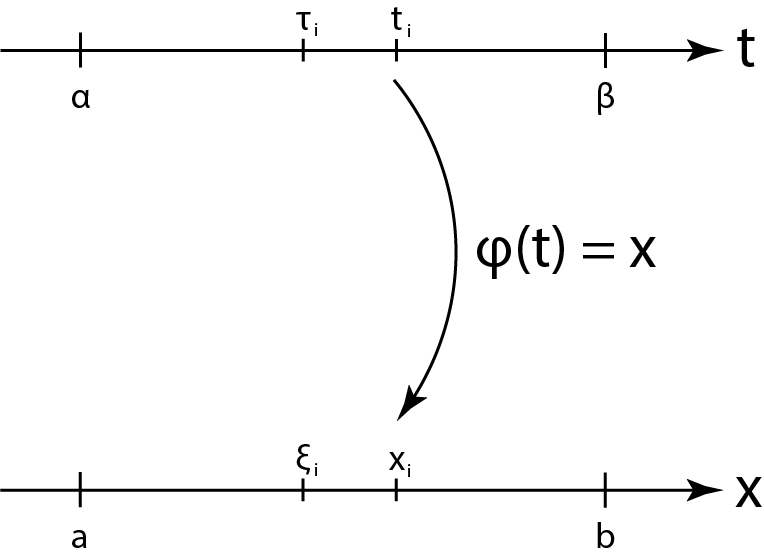
\includegraphics[scale=0.1]{graph5.png}}
    \end{minipage}
    \hfill
    \begin{minipage}[h]{0.49\linewidth}
      $a = x_0 < x_1 < \ldots < x_{n-1} < x_n = b;$

      $\xi_i \in [x_{i-1};x_i], \ i = \overline{1,n},$

      Здесь $x_i = \phi(t_i), \ \xi_i = \phi(\tau_i)$.
    \end{minipage}
  \end{figure}

  Если $\lambda(P_t)\rightarrow0 \implies \lambda(P_x)\rightarrow0$. Составим интегральные суммы:
  \begin{equation*}
    \sigma = \sum_{i=1}^{n}f(\phi(\tau_i))\phi'(\tau_i)\Delta t_i;
  \end{equation*}
  \begin{equation*}
    \overline{\sigma} = \sum_{i=1}^{n}f(\xi_i)\Delta x_i,
  \end{equation*}
  Если $\lambda(P_t)\rightarrow0 \implies \lambda(P_x) \rightarrow 0 \implies \overline{\sigma}
    \rightarrow \int_{a}^{b}f(x)dx$ (так как $f\in R[a;b]$).

  Покажем, что $\sigma \rightarrow \int_{a}^{b}f(x)dx: \ \Delta x_i = x_i - x_{i-1} = \phi(t_i)
    - \phi (t_{i-1}) = \phi'(\overline{\tau_i})\Delta t_i, \ \overline{\tau_i} \in [t_{i-1};t_i]$
  (случайная точка из отрезка).

  Тогда:
  \begin{equation*}
    \overline{\sigma} = \sum_{i=1}^{n}f(\xi_i)\Delta x_i = \sum_{i=1}^{n}f(\phi(\tau_i))
    \phi'(\overline{\tau_i})\Delta t_i;
  \end{equation*}
  Покажем, что $\underset{\lambda(P_i)\rightarrow0}{\lim}(\sigma - \overline{\sigma}) = 0:$

  В самом деле, $| \sigma - \overline{\sigma} | = | \sum_{i=1}^{n} f(\phi(\tau_i))\phi'(\tau_i)
    \Delta t_i - \sum_{i=1}^{n}f(\phi(\tau_i)\phi'(\overline{\tau_i}))\Delta t_i | =
    | \sum_{i=1}^{n}f(\phi(\tau_i))(\phi'(\tau_i) - \phi'(\overline{\tau_i}))\Delta t_i | \leqslant
    \sum_{i=1}^{n}| f(\phi(\tau_i)) | | \phi'(\tau_i) - \phi'(\overline{\tau_i}) |\Delta t_i \leqslant
    \\ L\sum_{i=1}^{n}| \phi'(\tau_i) - \phi'(\overline{\tau_i}) | \Delta t_i$, где $L>0: \ \forall x
    \in [a;b] \quad |f(x)| \leqslant L$ (так как $f$ - интегрируема $\implies$ ограничена).

  Так как $\phi'(t)$ непрерывна на $[\alpha;\beta] \implies \forall i = \overline{1,n} \
    \phi'(t)$ непрерывна на $[t_{i-1}; t_i] \implies \phi'(t)$ равномерно непрерывна на $[t_{i-1}; t_i]$.
  Возьмем $\delta > 0 : \ \forall t_1, t_2 \in [t_{i-1}; t_i] \ | [t_1 - t_2] | < \delta \implies
    | \phi'(t_1) - \phi'(t_2) | < \frac{\epsilon}{L(\beta - \alpha)} \ (\forall \epsilon > 0)$.

  Тогда $| \sigma - \overline{\sigma} | \leqslant L\sum_{i=1}^{n} | \phi'(\tau_i) - \phi'(\overline{
      \tau_i}) | \Delta t_i < L\frac{\epsilon}{L(\beta - \alpha)}\sum_{i=1}^{n}\Delta t_i = L
    \frac{\epsilon}{L(\beta - \alpha)}(\beta - \alpha) = \epsilon \implies \sigma \rightarrow
    \int_{a}^{b}f(x)dx$ при $\lambda(P_t) \rightarrow 0$.

  С другой стороны, по определению определенного интеграла:
  \begin{equation*}
    \underset{\lambda(P_t)\rightarrow0}{\lim}
    \sigma = \int_{\alpha}^{\beta}f(\phi(t))\phi'(t)dt \implies \int_{a}^{b}f(x)dx = \int_{\alpha}^{\beta}
    f(\phi(t))\phi'(t)dt.
  \end{equation*}
\end{proof}

\chapter{Геометрические приложения интеграла Римана}

\section{Длина кривой}

\begin{definition}
  Пусть $(X,\rho)$ - метрическое пространство, $[a;b] \subset \mathbb{R}$. Будем называть \textbf{путем}
  произвольное непрерывное отображение:
  \begin{equation*}
    \gamma:[a;b]\rightarrow X
  \end{equation*}
\end{definition}

\begin{definition}
  Пусть $\gamma:[a;b]\rightarrow X$ называется \textbf{простым}, если:
  \begin{equation*}
    \forall t_1,t_2 \in[a;b]: \quad \gamma(t_1) = \gamma(t_2) \implies t_1 = t_2
  \end{equation*}
  \begin{figure}[H]
    \begin{center}
      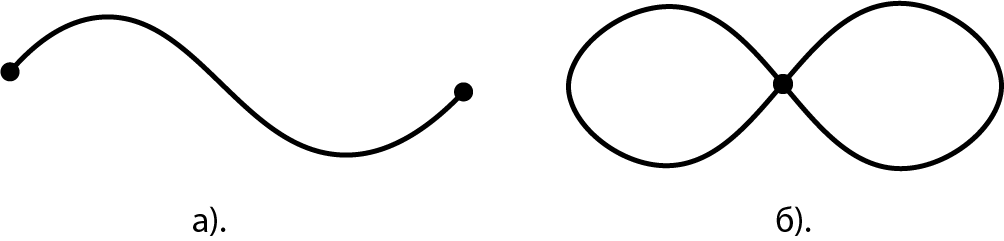
\includegraphics[scale=0.2]{graph6.png}\label{figure6}

      а). простой путь $\quad$ б). непростой путь
    \end{center}
  \end{figure}
\end{definition}

\begin{definition}
  Пусть $\gamma:[a;b]\rightarrow X$ называется \textbf{замкнутым}, если:
  \begin{equation*}
    \gamma(a) = \gamma(b),
  \end{equation*}
  тогда:
  \begin{itemize}
    \item $\gamma(a)$ - начало пути,
    \item $\gamma(b)$ - конец пути
  \end{itemize}
\end{definition}

\begin{definition}
  Пусть $\gamma:[a;b]\rightarrow X$ называется \textbf{простым замкнутым}, если:
  \begin{equation*}
    \forall t_1,t_2\in(a;b): \ \gamma(t_1)=\gamma(t_2)\implies t_1=t_2; \ \gamma(a) = \gamma(b)
  \end{equation*}
\end{definition}

\clearpage

На множестве путей введем отношение.

Пусть $\gamma_1:[a;b]\rightarrow X, \ \gamma_2:[\alpha;\beta] \rightarrow X$.

Будем говорить, что $\gamma_1$ и $\gamma_2$ находятся в отношении $"\sim"$, то есть $\gamma_1 \sim \gamma_2$,
если существует строго возрастающее отображение $\phi:[\alpha;\beta]\rightarrow[a;b]:$
\begin{equation*}
  \phi(\alpha) = a, \ \phi(\beta) = b,
\end{equation*}
а так же:
\begin{equation*}
  \gamma_2(\tau) = \gamma_1(\phi(\tau))
\end{equation*}
\begin{figure}[H]
  \begin{center}
    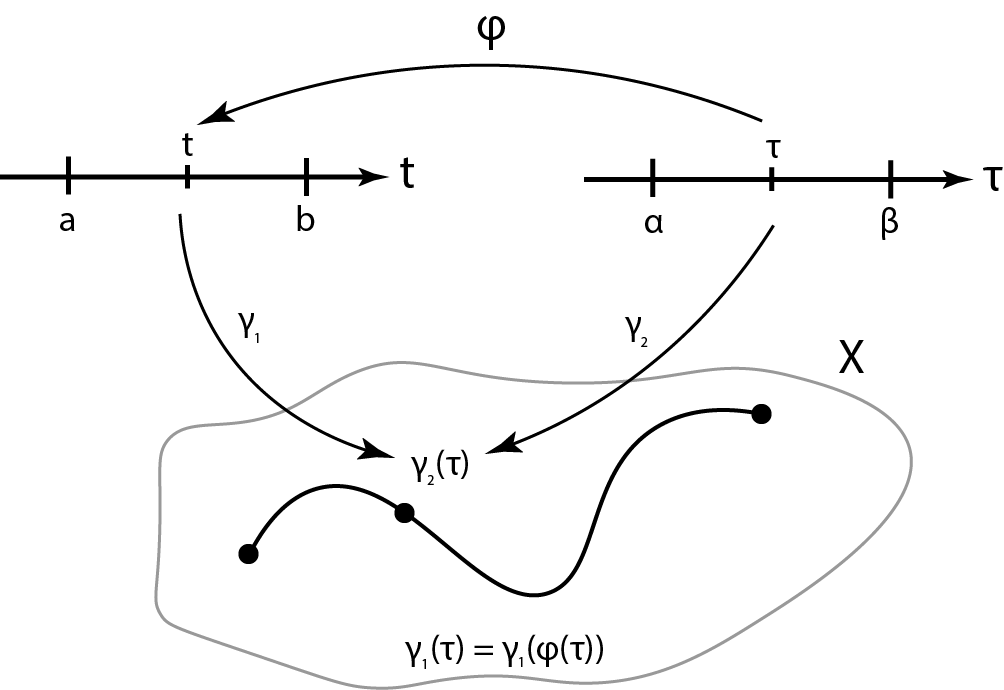
\includegraphics[scale=0.2]{graph7.png}\label{figure7}
  \end{center}
\end{figure}

Упражнение 1: Доказать, что введенное отношение есть отношение эквивалентности.

\begin{definition}
  Отображение $\phi$ называется \textbf{гомеоморфизмом}, если:
  \begin{center}
    $\phi$ и $\phi^{-1}$ - непрерывны
  \end{center}
\end{definition}

Упражнение 2: Доказать, что $\phi$ в определении отношения между $\gamma_1$ и $\gamma_2$ есть
гомеоморфизм.

\begin{definition}
  \textbf{Кривой} в $X$ будем называть класс эквивалентных путей.
\end{definition}

\begin{definition}
  Образ пути $\gamma$ называется \textbf{носителем} этого пути.
\end{definition}

\begin{example}
  Рассмотрим:

  $\gamma_1: [0;1] \rightarrow \mathbb{R}: \quad \gamma_1(t) = t$;

  $\gamma_2: [0;1] \rightarrow \mathbb{R}: \quad \gamma_2(\tau) = \tau^3$,

  \begin{figure}[H]
    \begin{center}
      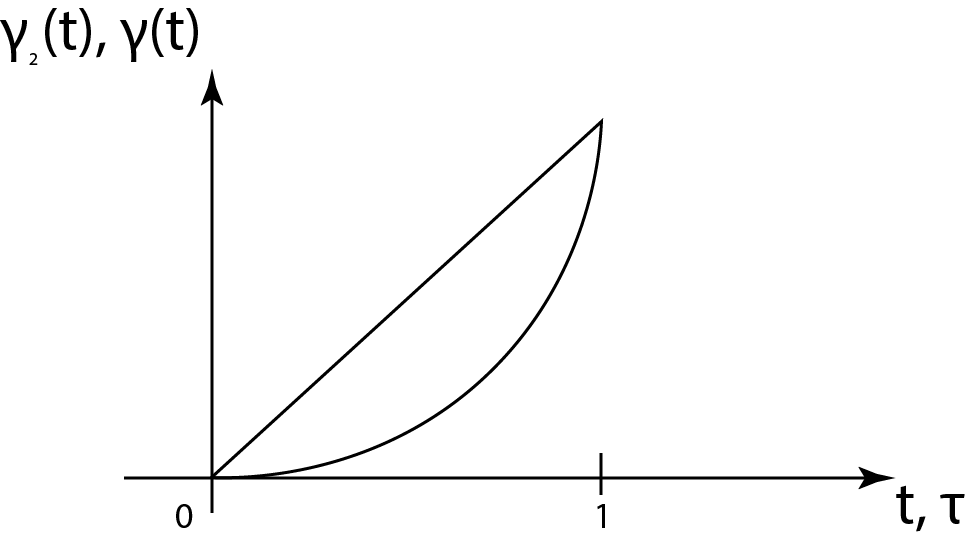
\includegraphics[scale=0.2]{graph8.png}\label{figure8}
    \end{center}
  \end{figure}

  Что бы доказать, что $\gamma_1 \sim \gamma_2$, нужно найти строго возрастающее отображение
  $\phi:[0;1]\rightarrow[0;1]$:

  $t = \phi(\tau) = \tau^3, \ \phi(\tau)$ - строго возрастающее, $\phi(0) = 0, \ \phi(1) = 1$;

  $\gamma_2(\tau) = \tau^3 = \phi(\tau) = t = \gamma_1(t) = \gamma_1(\phi(\tau)) \implies
    \gamma_2(\tau) = \gamma_1(\phi(\tau))$.
\end{example}

\begin{definition}
  Кривая называется \textbf{простой}, если она представляется простым путем (это значит, что в ее классе
  есть простой путь).
\end{definition}

Упражнение 3: Доказать, что если один путь в классе эквивалентности простой, то остальные тоже простые.

\begin{definition}
  Путь, представляющий данную кривую (из класса эквивалентности путей) $l$ называется
  \textbf{параметризацией} этой кривой.
\end{definition}

Вдальнейшем будем рассматривать метрические пространства $(X,\rho)$ как $\mathbb{R}^2, \ \mathbb{R}^3$
с евклидовой метрикой.

\begin{definition}
  Пусть $l$ - простая кривая в $\mathbb{R}^2, \ \gamma(t) = (x(t);t(t))$ - ее параметризация.
  Кривая $l$ называется \textbf{гладкой}, если $\forall t \ x(t),y(t)$ имеют непрерывные производные
  на $[\alpha,\beta]$ и $\nexists t_0 \in [\alpha,\beta] \ (\gamma : [\alpha,\beta] \rightarrow
    \mathbb{R}^2), \ x'(t_0)=0$ и $y'(t_0) = 0$.
\end{definition}

\begin{definition}
  Пусть $l \subset \mathbb{R}^2 \ (\mathbb{R}^3)$ и $\gamma:[\alpha,\beta]\rightarrow\mathbb{R}^2 \
    (\mathbb{R}^3)$ - параметризация кривой $l$.

  Пусть $\alpha = t_0 < t_1 < \ldots < t_{n-1} < t_n = \beta$ - разбиение отрезка $[\alpha,\beta]$
  и $M_i = \gamma(t_i), \ i=\overline{0,n}$ - точка пути $\gamma$ (кривая $l$):
  \begin{equation*}
    M_i = \gamma (t_i) = (x(t_i);y(t_i))
  \end{equation*}
  Тогда отрезок $M_{i-1}M_i \ (i = \overline{1,n})$ называется \textbf{звеном} кривой $l$.
  Объединение $\underset{i}{\cap}M_{i-1}M_i$ - ломаная, вписанная в $l$.

  \textbf{Периметром} ломаной называется сумма длин ее звеньев:
  \begin{equation*}
    p(M_0,M_1,\ldots,M_n) = \sum_{i=1}^{n}| M_{i-1}M_i |
  \end{equation*}
  \begin{figure}[h]
    \begin{minipage}[h]{0.49\linewidth}
      \center{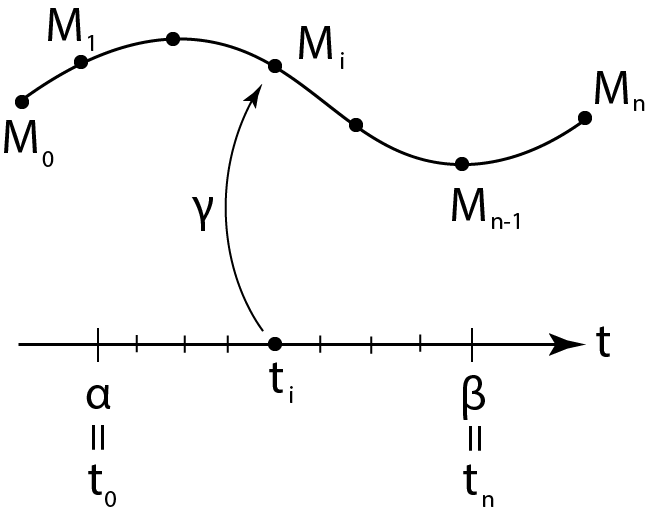
\includegraphics[scale=0.2]{graph9.png}}
    \end{minipage}
    \hfill
    \begin{minipage}[h]{0.49\linewidth}
      \center{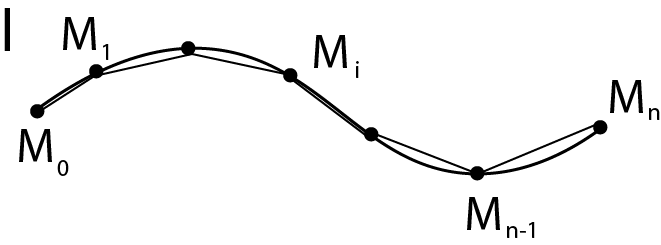
\includegraphics[scale=0.2]{graph10.png}}
    \end{minipage}
  \end{figure}
\end{definition}

\begin{definition}
  Если множество периметров ломаных, вписанных в данную кривую $l$ - ограничено, то кривую $l$
  будем называть \textbf{спрямляемой}.
\end{definition}

\begin{definition}
  Если $p(M_0,M_1,\ldots,M_n)$ - периметр ломаной, вписанной в кривую $l, \ S(l)$ - длина кривой, то
  по определению:
  \begin{equation*}
    S(l) = \sup p(M_0,\ldots,M_n),
  \end{equation*}
  где $\sup$ берется по всем ломаным $\underset{i}{\cup} M_{i-1}M_i$, вписанным в $l$.
\end{definition}

\begin{example}
  (неспрямляемой кривой)

  \begin{figure}[H]
    \begin{center}
      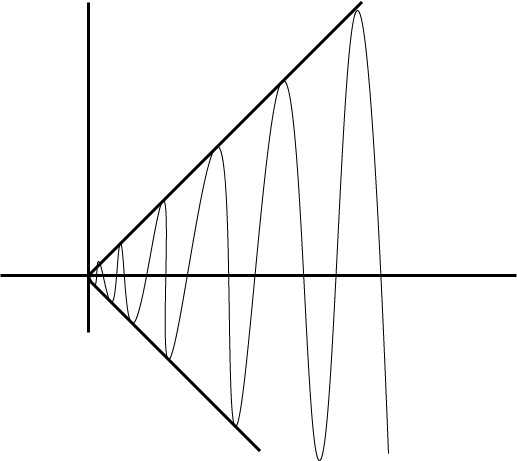
\includegraphics[scale=0.2]{graph11.png}\label{figure11}
    \end{center}
  \end{figure}
\end{example}

Рассмотрим $L$ - множество всех спрямляемых кривых на плоскости $(\mathbb{R}^2)$.
Введем $S:L\rightarrow\mathbb{R}$, то есть отображение $S$ сопоставляет спрямляемую кривую $l$
ее длину.
\begin{center}
  $S(l)$ - длина кривой $l$
\end{center}

\begin{theorem}[аддитивность длины кривой]
  Функция $S(l)$ является аддитивной, то есть если $l = l_1 \cup l_2$, то $S(l) = S(l_1) + S(l_2)$.

  \textbf{Более тонко:} Пусть $\gamma:[a;b]\rightarrow\mathbb{R}^2$ - параметризация спрямляемой кривой
  $l$, точка $c \in [a;b]$:

  $\gamma_1:[a;c] \rightarrow \mathbb{R}^2$ - параметризация кривой $l_1$,

  $\gamma_2:[c;b] \rightarrow \mathbb{R}^2$ - параметризация кривой $l_2$,

  при этом $C = \gamma(c) = \gamma_1(c) = \gamma_2(c)$.
  \begin{figure}[H]
    \begin{center}
      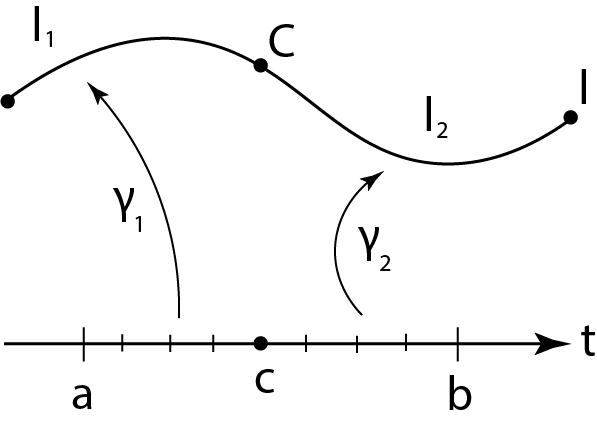
\includegraphics[scale=0.2]{graph12.png}\label{figure12}
    \end{center}
  \end{figure}

  Тогда $S(l) = S(l_1) + S(l_2)$.
\end{theorem}

\begin{proof}
  Пусть $l$ - спрямляемая кривая. Покажем, что $l_1$ и $l_2$ - спрямляемые.

  Обозначим за $m_1$ и $m_2$ - ломаные, вписанные в $l_1$ и $l_2$ соответственно. Тогда можно ввести
  $m$ как $m = m_1 \cup m_2$ - ломаная, вписанная в $l$.
  \begin{figure}[H]
    \begin{center}
      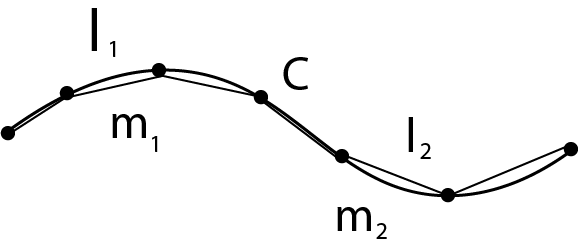
\includegraphics[scale=0.2]{graph13.png}\label{figure13}
    \end{center}
  \end{figure}

  $p(m)$ - периметр ломаной, вписанной в $l$, $p(m) = p(m_1) + p(m_2) \leqslant S(l) \implies
    p(m_1)\leqslant S(l)$ и $p(m_2) \leqslant S(l) \implies l_1$ и $l_2$ - спрямляемые.

  Пусть $S(l_1) = \underset{m_1}{\sup} p(m_1)$ и $S(l_2) = \underset{m_2}{\sup} p(m_2) \implies
    S(l_1) + S(l_2) \leqslant S(l)$

  Обратно, пусть $l_2$ и $l_2$ - спрямляемые кривые. Покажем, что $l$ - спрямляемая. Пусть $m$
  - некоторая ломаная, вписанная в $l$.

  Возьмем $C \in l$. Пусть $m'$ - ломаная, получаемая из ломаной $m$ добавлением звеньев,
  проходящих через $C$.
  \begin{figure}[h]
    \begin{minipage}[h]{0.49\linewidth}
      \center{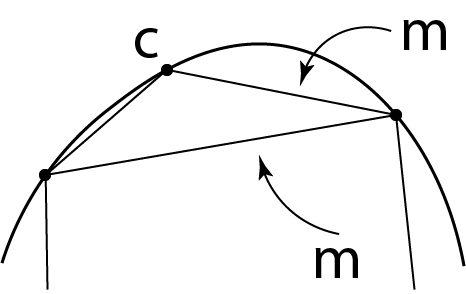
\includegraphics[scale=0.2]{graph14.png}}
    \end{minipage}
    \hfill
    \begin{minipage}[h]{0.49\linewidth}
      Пусть $m_1$ - часть ломаной, вписанной в $l_1, \ m_2'$ - часть ломаной, вписанной
      в $l_2$. Тогда $p(m) \leqslant p(m') = p(m_1') + p(m_2') \leqslant S(l_1) + S(l_2) \implies
        S(l) = \underset{m}{p(m)} \leqslant S(l_1) + S(l_2)$.
    \end{minipage}
  \end{figure}



  Тогда имеем, что $S(l_1) + S(l_2) \leqslant S(l) \leqslant S(l_1) + S(l_2) \implies S(l) =
    S(l_1) + S(l_2)$.
\end{proof}

\section{Длина кривой как предел}

\begin{theorem}
  Пусть $l$ - простая спрямляемая незамкнутая кривая в $\mathbb{R}^2$ и $\gamma:[a;b]\rightarrow\mathbb{R}^2$
  - ее параметризация. Пусть $a = t_0 < t_1 < \ldots < t_{n-1} < t_n = b$ - разбиение отрезка $[a;b]$,
  этому разбиению соответствуют точки $M_0,M_1,\ldots,M_n$ - соответсвующая ломаная, вписанная в $l \
    (M_i = \gamma(t_i))$, тогда:
  \begin{equation*}
    S(l) = \underset{\lambda\rightarrow0}{\lim}p(m),
  \end{equation*}
  где $\lambda = \underset{i}{\max}\Delta t_i, \ \Delta t_i = t_i - t_{i-1}$.
\end{theorem}

\begin{proof}
  (теоремы) Пусть $l$ - простая спрямляемая незамкнутая кривая в $\mathbb{R}^2, \ P' =
    \{a=t_0<t_1<\ldots<t_{n-1} <t_n=b\}$ - произвольное разбиение отрезка $[a;b]$.

  $m(P')$ - ломаная, вписанная в $l$, соответствующая разбиениею $P$. Пусть $\gamma:[a;b]\rightarrow
    \mathbb{R}^2$ - параметризация кривой $l, \ \gamma(t) = (x(t);y(t)), \ t\in[a;b]$.
  \begin{lemma}
    Если разбиение $P''$ получено из разбиения $P'$ добавлением точки на промежуток $(t_{i-1};t_i)$,
    то периметр ломаной, соответсвующий разбиению $P'$, не больше периметра ломаной, соответсвующей
    разбиению $P''$ и $p(m(P')) \leqslant p(m(P'')) \leqslant p(m(P')) + 2(\omega_i(x(t)) + \omega_i(y(t)))$, где
    $\omega_i$ - колебания функции $x(t), \ y(t)$:
    \begin{equation*}
      \omega_i(x(t)) = \underset{t',t''\in[t_{i-1};t_i]}{\sup}(x(t') - x(t'')) =
      \underset{t\in[t_{i-1};t_i]}{\sup}(x(t)) - \underset{t\in[t_{i-1};t_i]}{\inf}(x(t))
    \end{equation*}
    \begin{figure}[H]
      \begin{center}
        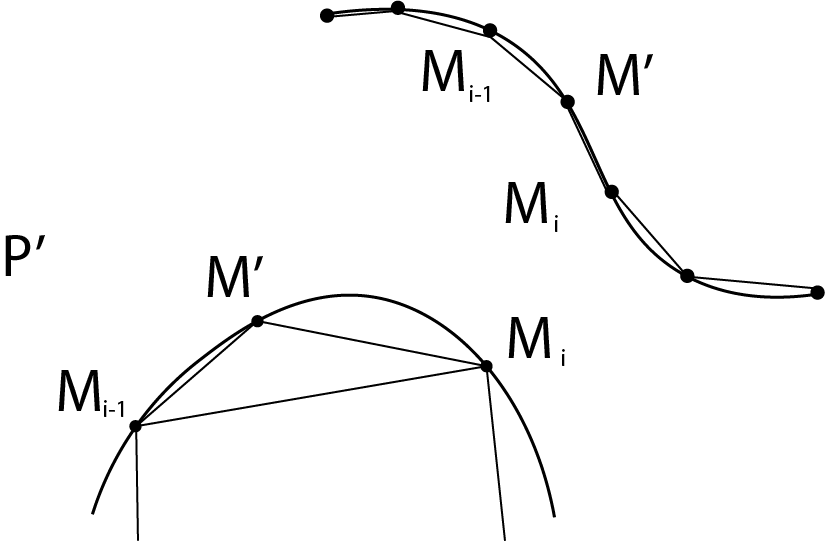
\includegraphics[scale=0.2]{graph15.png}\label{figure15}
      \end{center}
    \end{figure}
  \end{lemma}
  \begin{proof}
    (леммы) Ломаная $m(P'')$ получена из ломаной $m(P')$ путем замены звена $M_{i-1}M_i$ на два
    звена: $M_{i-1}M'$ и $M'M_i$.

    Очевидно, что $p(m(P')) \leqslant p(m(P''))$.
    \begin{figure}[h]
      \begin{minipage}[h]{0.49\linewidth}
        \center{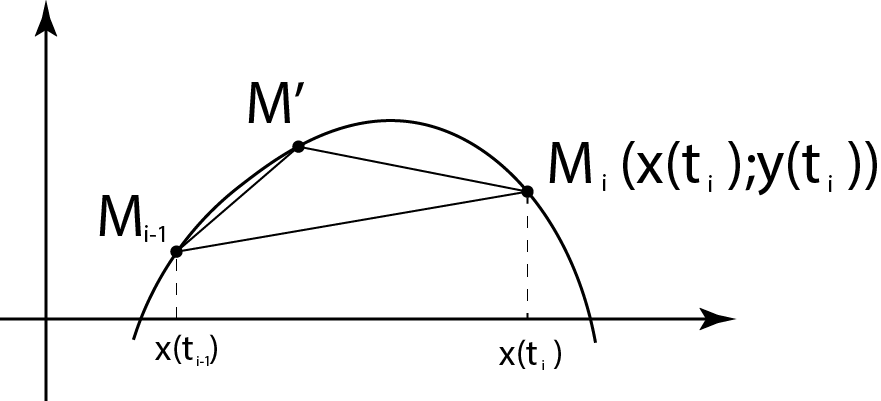
\includegraphics[scale=0.15]{graph16.png}}
      \end{minipage}
      \hfill
      \begin{minipage}[h]{0.49\linewidth}
        $M_i = \gamma (t_i) = (x(t_i);y(t_i)), \ M' = (x(t');y(t')), \ M_{i-1} =
          (x(t_{i-1});y(t_{i-1}))$

        $| M_{i-1}M' | + | M'M_i | \leqslant | x(t') - x(t_{i-1}) | + | y(t') - y(t_{i-1}) | + | x(t_i) - x(t') |
          + | y(t_i) - y(t') | \leqslant 2\omega_i(x(t)) + 2\omega_i(y(t)), \ \sup$ берется на отрезке
        $[t_{i-1};t_i]$.
      \end{minipage}
    \end{figure}

    В итоге, $p(m(P'')) \leqslant p(m(P')) + 2(\omega_i(x(t)) + \omega_i(y(t)))$.

    Если не понятно: $p(m(P'')) = \sum_{k=1}^{n}| M_{k-1} M_k | = \sum_{k=1}^{i-1}| M_{k-1}M_k | +
      | M_{i-1}M' | + | M'M_i | + \sum_{k=i+1}^{n}| M_{k-1}M_k | \leqslant p(m(P')) + 2(\omega_i(x(t))
      +\omega_i(y(t)))$.
  \end{proof}

  (повтор) Пусть $\epsilon > 0$ задано. Выберем произвольное разбиение $P'$ отрезка $[a;b]: \ p(m(P'))
    > S(l) - \frac{\epsilon}{2}$ (по определению $\sup$ множества).

  Пусть это разбиение состоит из $n$ точек. Тогда выберем $\delta > 0: \ \forall t',t'' \in [a;b]: \
    |t'-t''| < \delta \implies | x(t') - x(t'') | < \frac{\epsilon}{8n}; \ | y(t') - y(t'') | < \frac{\epsilon}
    {8n}$.

  Пусть $P''$ - произвольное разбиение: $\lambda(P'') < \delta$. Покажем, что $p(m(P'')) \leqslant S(l)$
  и $p(m(P'')) > S(l) - \frac{\epsilon}{2}$.

  Рассмотрим $P''' = P' \cup P''$. Тогда $p(m(P''')) \geqslant p(m(P''))$. С другой стороны, $P'''$
  получена из $P''$ добавлением не более чем $n$ точек. Тогда $p(m(P''')) \leqslant p(m(P'')) +
    \sum_{i=1}^{n}2(\omega_i(x(t)) + \omega_i(y(t))) < S(l) + 4 \frac{\epsilon}{8n}n = S(l) +
    \frac{\epsilon}{2}$. Получим, что:
  \begin{equation*}
    p(m(P''')) < S(l) + \frac{\epsilon}{2}.
  \end{equation*}

  Так как $P'''$ тоже получено из $P'$ добавлением точек, то:
  \begin{equation*}
    p(m(P''')) \geqslant p(m(P')) > S(l) - \frac{\epsilon}{2}.
  \end{equation*}

  Так же имеем, что $p(m(P''')) \leqslant p(m(P'')) + \frac{\epsilon}{2} \implies p(m(P'')) \geqslant
    p(m(P''')) - \frac{\epsilon}{2} \geqslant p(m(P')) - \frac{\epsilon}{2} > S(l) - \frac{\epsilon}{2}
    - \frac{\epsilon}{2} = S(l) - \epsilon$.

  Так как $S(l) = \underset{m}{\sup} p(m(P)), \ P$ - разбиение отрезка $[a;b] \implies$
  \begin{equation*}
    p(m(P'')) \leqslant S(l) < S(l) + \epsilon.
  \end{equation*}

  Таким образом, если $\epsilon > 0$ задано, то возьмем произвольное разбиение $P'': \ \lambda(P'') <
    \delta \implies S(l) - \epsilon < p(m(P'')) < S(l) + \epsilon \implies | p(m(P'')) - S(l) | < \epsilon
    \implies$
  \begin{equation*}
    \underset{\lambda(P)\rightarrow0}{\lim}p(m(P'')) = S(l).
  \end{equation*}
\end{proof}

\begin{theorem}[формула для вычисления длины кривой]
  Пусть $l$ - гладкая кривая; $\gamma:[a;b]\rightarrow\mathbb{R}^2$ - ее параметризация (гладкая,
  то есть $\gamma(t) = (x(t);y(t))$, где $x(t)$ и $y(t)$ имеют непрерывные произведения на $[a;b]$).
  Тогда $l$ - спрямляема и:
  \begin{equation*}
    S(l) = \int_{a}^{b}\sqrt{(x'(t))^2 + (y'(t))^2}dt
  \end{equation*}
\end{theorem}

\begin{proof}
  (теоремы) Возьмем разбиение:
  \begin{equation*}
    P' = \{a=t_0<t_1<\ldots<t_{n-1}<t_n=b\}
  \end{equation*}
  Тогда:
  \begin{equation*}
    p(m(P')) = \sum_{i=1}^{n} \sqrt{(x(t_i)) - x(t_{i-1})^2 + (y(t_i) - y(t_{i-1}))^2}
  \end{equation*}
  $\forall i = \overline{1,n} \ x(t_i) - x(t_{i-1}) = x'(\tau_i)\Delta t_i, \ \tau_i\in[t_{i-1};t_i], \
    y(t_i) - y(t_{i-1}) = y'(\overline{\tau_i})\Delta t_i, \ \overline{\tau_i}\in[t_{i-1};t_i]$.

  Тогда:
  \begin{equation*}
    p(m(P')) = \sum_{i=1}^{n}\sqrt{(x'(\tau_i)\Delta t_i)^2 + (y'(\overline{\tau_i})\Delta t_i)^2} =
    \sum_{i=1}^{n}\sqrt{(x'(\tau_i))^2 + (y'(\overline{\tau_i}))^2}\Delta t_i.
  \end{equation*}

  Рассмотрим функцию:
  \begin{equation*}
    \phi(t) = \sqrt{(x'(t))^2 + (y'(t))^2},
  \end{equation*}
  где $\phi(t)$ - непрерывна на $[a;b] \implies \phi(t)$ - интегрируема на $[a;b]$, то есть:
  \begin{equation*}
    \exists \underset{\lambda(P')\rightarrow0}{\lim}\sigma = \int_{a}^{b}\phi(t)dt,
  \end{equation*}
  где $\sigma = \sum_{i=1}^{n}\phi(\tau_i)\Delta t_i = \sum_{i=1}^{n}\sqrt{(x'(\tau_i))^2 +
      (y'(\tau_i))^2}\Delta t_i$.

  \begin{lemma}
    $\forall a,b_1,b_2\in\mathbb{R}$ верно неравенство:
    \begin{equation*}
      \sqrt{a^2 + b_1^2} - \sqrt{a^2 + b_2^2} \leqslant | b_1 - b_2 |
    \end{equation*}
  \end{lemma}

  \begin{proof}
    (леммы)

    \begin{enumerate}
      \item Если $a=0$ - очевидно;
      \item Если $a\ne0 \implies \frac{(\sqrt{a^2 + b_1^2} - \sqrt{a^2 + b_2^2})
                (\sqrt{a^2 + b_1^2} - \sqrt{a^2 + b_2^2})}{\sqrt{a^2 + b_1^2} - \sqrt{a^2 + b_2^2}} =
              \frac{| b_1^2 - b_2^2 |}{\sqrt{a^2 + b_1^2} - \sqrt{a^2 + b_2^2}} =
              \frac{| b_1 + b_2 | | b_1 - b_2 |}{\sqrt{a^2 + b_1^2} - \sqrt{a^2 + b_2^2}} <
              \frac{| b_1 + b_2 |}{| b_1 | + | b_2 |}| b_1 - b_2 | \leqslant | b_1 - b_2 |$, потому что
            $\frac{| b_1 + b_2 |}{| b_1 | + | b_2 |} \leqslant 1$.
    \end{enumerate}
  \end{proof}

  Покажем, что:
  \begin{equation*}
    \underset{\lambda(P')\rightarrow0}{\lim}(p(m(P')) - \sigma) = 0.
  \end{equation*}

  $| p(m(P')) - \sigma | = | \sum_{i=1}^{n}\sqrt{(x'(\tau_i))^2 + (y'(\overline{\tau_i}))^2}\Delta t_i
    - \sum_{i=1}^{n}\sqrt{(x'(\tau_i))^2 + (y'(\tau_i))^2}\Delta t_i | = | \sum_{i=1}^{n}(
    \sqrt{(x'(t_i))^2 + (y'(\overline{\tau_i}))^2} - \sqrt{(x'(\tau_i))^2 + (y'(\tau_i))^2})\Delta t_i |
    \leqslant \sum_{i=1}^{n} | \sqrt{(x'(\tau_i))^2 + (y'(\overline{\tau_i}))^2} -
    \sqrt{(x'(\tau_i))^2 + (y'(\tau_i))^2} | \Delta t_i \overset{lemma}{\leqslant} \sum_{i=1}^{n}
    | y'(\overline{\tau_i}) - y'(\tau_i) |\Delta t_i \leqslant \sum_{i=1}^{n}\omega_i(y'(t))\Delta t_i $

  Напоминание:
  \begin{equation*}
    \omega_i(t) = \underset{t',t''\in[t_{i-1};t_i]}{\sup}| f(t') - f(t'') |
  \end{equation*}

  Так как $y'(t)$ - непрерывная функция $\implies y'(t)$ - интегрируема на $[a;b] \implies
    \sum_{i=1}^{n} \omega_i(y')\Delta t_i \rightarrow 0$ (по критерию интегрируемости) $\implies$
  \begin{equation*}
    \underset{\lambda(P')\rightarrow0}{\lim} (p(m(P')) - \sigma) = 0.
  \end{equation*}

  $\underset{\lambda(P')\rightarrow0}{\lim}(p(m(P'))) = \underset{\lambda(P')\rightarrow0}{\lim}\sigma
    = \int_{a}^{b}\sqrt{(x'(t))^2 + (y'(t))^2}dt$.
\end{proof}

\begin{effect}
  (теоремы)

  \begin{enumerate}
    \item Пусть $l$ - график функции $y=y(x)$.

          Тогда:
          \begin{equation*}
            \left\{
            \begin{array}{ll}
              x = x \\
              y=y(x)
            \end{array}
            \right. \implies S(l) = \int_{a}^{b}\sqrt{1 + (y'(x))^2}dx
          \end{equation*}

    \item Пусть $r = r(\phi)$ - уравнение кривой в полярной системе координат.

          $x = r\cos\phi, \quad y = r\sin\phi, \quad \phi\in[\alpha,\beta]$.
          Тогда:
          \begin{equation*}
            \left\{
            \begin{array}{ll}
              x(\phi) = r(\phi)\cos\phi \\
              y(\phi) = r(\phi)\sin\phi
            \end{array}
            \right. \implies
            \left\{
            \begin{array}{ll}
              x'(\phi) = r'(\phi)\cos\phi - r(\phi)\sin\phi \\
              y'(\phi) = r'(\phi)\sin\phi + r(\phi)\cos\phi
            \end{array}
            \right.
          \end{equation*}

          $(x'(\phi))^2 + (y'(\phi))^2 = (r')^2\cos^2\phi - 2r'r\sin\phi\cos\phi + r^2\sin^2\phi + (r')^2
            \sin^2\phi + 2r'r\sin\phi\cos\phi + r^2\cos^2\phi = (r')^2 + r^2$.

          Тогда формула для вычисления длины кривой в полярной системе координат:
          \begin{equation*}
            S(l) = \int_{\alpha}^{\beta}\sqrt{(r'(\phi))^2 + (r(\phi))^2}d\phi
          \end{equation*}
  \end{enumerate}
\end{effect}

\section{Площадь плоской фигуры}

\begin{definition}
  \textbf{Многоугольник} - множество точек плоскости, границей которого является объединение конечного
  числа непересекающихся простых ломаных, при этом это объединение само является замкнутой ломаной.
  \begin{figure}[H]
    \begin{center}
      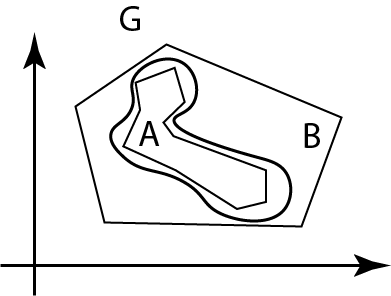
\includegraphics[scale=0.3]{graph17.png}\label{figure17}
    \end{center}
  \end{figure}
\end{definition}


\begin{definition}
  Пусть $G$ - множество на плоскости, $G\subset\mathbb{R}^2$. Будем говорить, что многоугольник $A$
  \textbf{вписан} в $G$, если $A \subset G$ и $A$ \textbf{описан около} $G$, если $G \subset A$.
\end{definition}

\begin{definition}
  Множество $G\subset\mathbb{R}^2$ называется \textbf{измеримым по Жардану} (или \textbf{квадрируемым}),
  если:
  \begin{equation*}
    S_* = \underset{A\subset G}{\sup} S(A) = S^* = \underset{B\supset G}{\inf}S(B),
  \end{equation*}
  где $\sup$ берется по всем многоугольникам, вписанным в $G$, а $\inf$ - по всем многоугольникам,
  описанным около $G$. При этом их общее значение $S = S_* = S^*$ называется \textbf{площадью} $G$,
  или \textbf{мерой Жардана}.
  \begin{center}
    $S_*$ - \textbf{внутренняя} мера, $S^*$ - \textbf{внешняя} мера.
  \end{center}

  Другими словами, множество $G\subset\mathbb{R}^2$ квадрируемо, если внутреняя и внешняя меры совпадают.

  Здесь $S(A),\ S(B)$ - площади многоугольников $A$ и $B$. Многоугольник $A$ можно разбить на конечное число
  прямоугольников и прямоугольных треугольников:
  \begin{figure}[h]
    \begin{minipage}[h]{0.49\linewidth}
      \center{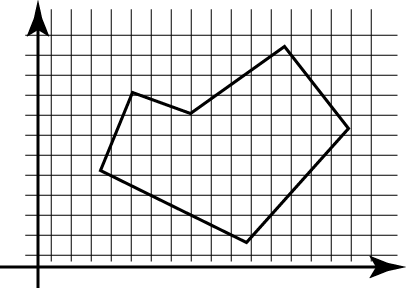
\includegraphics[scale=0.2]{graph18.png}}
    \end{minipage}
    \hfill
    \begin{minipage}[h]{0.49\linewidth}
      $S_\square = ab; \quad S_\triangle = \frac{1}{2}ab$
    \end{minipage}
  \end{figure}
\end{definition}

\begin{example}
  (из определения)

  \begin{enumerate}
    \item Квадрируемые множетсва на плоскости.

          Круг с границей:
          \begin{equation*}
            x^2 + y^2 = 1
          \end{equation*}
          Упражнение: доказать, что круг - квадрируемое множество.
    \item Неквадрируемые множества на плоскости.

          Множество точек одинарного квадрата с рациональными координатами:
          \begin{equation*}
            G = (\mathbb{Q} \times \mathbb{Q})\cap([0;1] \times [0;1])
          \end{equation*}
          Вписанный многоугольник $A = \emptyset, \ S(A) = 0$. Многоугольник $B = [0;1] \times [0;1]$
          имеет площадь равную  $1$ ($S(B) = 1$).
          \begin{equation*}
            S_* = 0, \quad S^* = \underset{B'\supset G}{\inf}S(B') = S(B) = 1 \ (S_* \ne S^*)
          \end{equation*}
  \end{enumerate}
\end{example}

\begin{theorem}[критерий квадрируемости]
  Множество $G\subset\mathbb{R}^2$ квадрируемо $\iff \forall \epsilon > 0 \ \exists$ многоугольники $A$ и $B$:
  \begin{enumerate}
    \item $A\subset G, \ B \supset G$,
    \item $S(B) - S(A) < \epsilon$.
  \end{enumerate}
\end{theorem}

\begin{proof}
  (теоремы)

  $" \rightarrow "$ Пусть $G \subset \mathbb{R}^2$ квадрируемо $\implies S_* = S^* = S'$.

  Выберем $A\subset G: \ S(A) > S - \frac{\epsilon}{2}$ ($\epsilon>0$ - задано) - по определению $\sup$.

  Выберем $B\supset G: \ S(B) < S + \frac{\epsilon}{2}$.
  \begin{equation*}
    S(B) - S(A) < (S + \frac{\epsilon}{2}) - (S - \frac{\epsilon}{2}) = \epsilon
  \end{equation*}

  $" \leftarrow "$ Пусть $\forall \epsilon > 0 \ \exists$ многоугольники $A$ и $B$, $A \subset G$,
  $B \supset G$ и $S(B) - S(A) < \epsilon$. Докажем, что $G$ - квадрируемо.

  \begin{equation*}
    S(B) - S(A) < \epsilon \implies S(B) - \epsilon < S(A) \leqslant S_* \leqslant S^* \leqslant S(B)
  \end{equation*}

  Так как $S(B) - S(A) < \epsilon \implies S^* - S_* < \epsilon$. Так как $\epsilon > 0$ - произвольное число
  $\implies S^* = S_*$, то есть $G$ - квадрируемо.
\end{proof}

\section{Классы квадрируемых областей}

\begin{definition}
  \textbf{Криволинейная трапеция} - часть плоскости, ограниченная прямыми $x=a, \ x=b$, графиком функции
  $y = f(x)$ и осью $Ox$. {\Large РИСУНОК}
\end{definition}

\begin{theorem}
  Криволинейная трапеция квадрируема и ее площадь равна:
  \begin{equation*}
    S = \int_{a}^{b}f(x)dx,
  \end{equation*}
  где $f(x)$ - непрерывна на $[a;b], \ f(x) \geqslant 0$.
\end{theorem}

\begin{proof}
  $ABCD$ - криволинейная трапеция, ограничена $x=a, \ x=b, \ y=0$, а так же графиком функции $y = f(x)$.
  Пусть $\epsilon > 0$ задано. Выберем $\delta>0: \ \forall x',x'':  \ | x' - x'' | < \delta \implies
    | f(x') - f(x'') | < \frac{\epsilon}{b - a}$ (так как $f(x)$ - непрерывна на $[a;b] \implies f(x)$
  равномерно непрерывна на $[a;b]$). {\Large РИСУНОК}

  Разобьем отрезок $[a;b]$ точками $a=x_0 < x_1 <\ldots < x_{n-1} < x_n = b$, таким образом, что бы
  $\underset{i}{\max}| x_i - x_{i-1} | < \delta$. Пусть:
  \begin{equation*}
    m_i = \underset{x\in[x_{i-1};x_i]}{\min}f(x), \ M_i = \underset{x\in[x_{i-1};x_i]}{\max}f(x).
  \end{equation*}

  Построим многоугольник $A$, вписанный в $ABCD$ и многоугольник $B$, описанный около $ABCD$. Многоугольник
  $A$ состоит из прямоугольников со сторонами $\Delta x_i$ и $m_i$, многоугольник $B$ состоит из прямоугольников
  со сторонами $\Delta x_i$ и $M_i$.
  \begin{equation*}
    S(A) = \sum_{i=1}^{n}m_i\Delta x_i, \quad S(B) = \sum_{i=1}^{n}M_i\Delta x_i,
  \end{equation*}
  \begin{equation*}
    S(B) - S(A) = \sum_{i=1}^{n}(M_i - m_i)\Delta x_i < \sum_{i=1}^{n}\frac{\epsilon}{b-a}\Delta x_i =
  \end{equation*}
  \begin{equation*}
    = \frac{\epsilon}{b-a}\sum_{i=1}^{n}\Delta x_i = \frac{\epsilon}{b-a}(b-a) = \epsilon \implies
  \end{equation*}
  по критерию квадрируемости, криволинейная трапеция $ABCD$ - квадрируема $\implies S_* = S^* = S_{ABCD}$.
  С другой стороны, $S(B) - S(A) = \sum_{i=1}^{n}(M_i - m_i)\Delta x_i \leqslant \sum_{i=1}^{n}\omega_i
    (f(x))\Delta x_i$.

  Так как $f$ - непрерывна на $[a;b] \implies f\in R[a;b] \implies \sum_{i=1}^{n}\omega_i\Delta x_i
    \rightarrow 0 \implies S_{ABCD} = \int_{a}^{b} = \int_{a}^{b}f(x)dx = S^* = S_*$.
\end{proof}

\begin{definition}
  Фигура на плоскости, ограниченная лучами $\phi = \alpha$ и $\phi = \beta$ и кривой $\rho = \rho(\phi)$
  называется \textbf{криволинейным сектором}.
\end{definition}

\begin{theorem}
  Пусть криволинейный сектор $\Omega$ ограничен лучами $\phi = \alpha, \ \phi = \beta$ и кривой $\rho
    = \rho(\phi)$. Тогда:
  \begin{equation*}
    S(\Omega) = \frac{1}{2}\int_{\alpha}^{\beta}\rho^2(\phi)d\phi,
  \end{equation*}
  где $\rho(\phi)$ - непрерывна на $[\alpha;\beta]$. {\Large РИСУНОК}
\end{theorem}
\begin{proof}
  Разобьем сектор $\Omega$ лучами $\alpha = \phi_0<\phi_1<\ldots<\phi_{n-1}<\phi_n=b$. Пусть:
  \begin{equation*}
    m_i = \underset{\phi\in[\phi_{i-1};\phi_i]}{\min}\rho(\phi), \quad M_i = \underset
    {\phi\in[\phi_{i-1};\phi_i]}{\max}\rho(\phi).
  \end{equation*}
  Построим криволинейные сектора с радиусами $m_i$ и $M_i$. Пусть $\underline{\Omega}$ - объединение
  секторов в радиусом $m_i$, а $\overline{\Omega}$ - объединение секторов с радиусом $M_i$.
  \begin{equation*}
    S(\underline{\Omega}) = \sum_{i=1}^{n}\pi m_i^2\frac{\Delta\phi_i}{2\pi}=\frac{1}{2}\sum_{i=1}^{n}
    m_i^2\Delta \phi_i,
  \end{equation*}
  \begin{equation*}
    S(\overline{\Omega}) = \sum_{i=1}^{n}\pi M_i^2\frac{\Delta\phi_i}{2\pi}=\frac{1}{2}\sum_{i=1}^{n}
    M_i^2\Delta \phi_i.
  \end{equation*}
  Заметим, что $S(\underline{\Omega})\leqslant S_{kriv.sector} \leqslant S(\overline{\Omega}) \ (*)$.

  Заметим, что $S(\underline{\Omega})$ - нижняя интегральная сумма функции $\frac{\rho^2(\phi)}{2}$,
  а $S(\overline{\Omega})$ - верхняя интегральная сумма этой же функции. Функция $\frac{\rho^2(\phi)}{2}$
  - непрерывна (так как $\rho(\phi)$ - непрерывна) $\implies$ интегрируема на $[\alpha;\beta] \implies
    \exists \underset{\max\Delta \phi_i\rightarrow0}{\lim}S(\underline{\Omega}) =
    \underset{\max\Delta \phi_i\rightarrow0}{\lim}S(\overline{\Omega}) = \int_{\alpha}^{\beta}\frac{\rho^2(\phi)}
    {2}d\phi \implies$ учитывая неравенство (*) и лемму о двух миллиционерах:
  \begin{equation*}
    S_{kriv.sector} = \frac{1}{2}\int_{\alpha}^{\beta}\rho^2(\phi)d\phi
  \end{equation*}
  и криволинейный сектор - квадрируемый.
\end{proof}

\chapter{Несобственные интегралы}

\begin{definition}
  Пусть $f:[a;+\infty)\rightarrow\mathbb{R}$ (задана на луче) и $\forall b \in [a;+\infty) \ f\in R[a;b]$.
  Рассмотрим:
  \begin{equation*}
    \underset{b\rightarrow+\infty}{\lim}\int_{a}^{b}f(x)dx,
  \end{equation*}
  этот предел называется \textbf{несобственным интегралом} от функции $f(x)$ на луче $[a;+\infty)$.

  Если этот предел существует и конечен, то несобственный интеграл называется \textbf{сходящимся}, иначе
  \textbf{расходящимся}. Обозначение:
  \begin{equation*}
    \int_{a}^{+\infty}f(x)dx \overset{def}{=}\underset{b\rightarrow+\infty}{\lim}\int_{a}^{b}f(x)dx
  \end{equation*}
\end{definition}

\begin{definition}
  (продолжение определения)

  \begin{enumerate}
    \item $\int_{2}^{+\infty}\frac{dx}{x^2} = \underset{b\rightarrow\infty}{\lim}\int_{2}^{b}\frac{dx}{x^2} =
            \underset{b\rightarrow+\infty}{\lim}(F(b) - F(2)) = \underset{b\rightarrow+\infty}{\lim}(-\frac{1}{b} +
            \frac{1}{2}) = \frac{1}{2}$.

          Аналогично, пусть функция $f:(-\infty;a]\rightarrow\mathbb{R}, \ f\in R[a;b], \ \forall b \in (-\infty;a]$.
          \begin{equation*}
            \underset{b\rightarrow-\infty}{\lim}\int_{a}^{b}f(x)dx,
          \end{equation*}
          этот предел называется \textbf{несобственным интегралом} от функции $f(x)$ на луче $(\infty;a]$.

          Если этот предел существует и конечен, то соответственно несобственный интеграл - сходящийся. Обозначается:
          \begin{equation*}
            \int_{-\infty}^{a}f(x)dx \overset{def}{=}\underset{b\rightarrow-\infty}{\lim}\int_{b}^{a}f(x)dx.
          \end{equation*}
          Аналогично:
          \begin{equation*}
            \int_{-\infty}^{+\infty}f(x)dx = \int_{-\infty}^{a}f(x)dx + \int_{a}^{+\infty}f(x)dx = \underset{c
              \rightarrow+\infty, b\rightarrow-\infty}{\lim}\int_{b}^{c}f(x)dx,
          \end{equation*}
          где $c\rightarrow+\infty, b\rightarrow-\infty$ - независимые друг от друга ($\forall b,c \ f(x)\in
            R[b;c]$). {\Large РИСУНОК}

    \item Далее, пусть $f:[a;b)\rightarrow\mathbb{R}: \ \forall c \in [a;b) f\in R[a;c]$. Положим:
                \begin{equation*}
                  \int_{a}^{b}f(x)dx = \underset{c\rightarrow b}{\lim}\int_{a}^{c}f(x)dx.
                \end{equation*}
                Эта величина называется \textbf{несобственным интегралом} от функции $f$ на полуинтервале $[a;b)$.

                    Если предел существует, то несобственный интеграл называется \textbf{сходящимся}, иначе \textbf{расходящимся}.

                    Аналогично, пусть $f:(a;b]\rightarrow\mathbb{R}$, причем $\forall c \in (a;b] \ f\in R[c;b]$:
          \begin{equation*}
            \int_{a}^{b}f(x)dx \overset{def}{=} \underset{c\rightarrow a}{\lim}\int_{c}^{b}f(x)dx \ -
          \end{equation*}
          несобственный интеграл от функции $f(x)$ на полуинтервале $(a;b]$.

          Аналогично, пусть $f:(a;b)\rightarrow\mathbb{R}$, причем $\forall c,d \in (a;b) \ f\in R[c,d]$.
          Тогда:
          \begin{equation*}
            \int_{a}^{b}f(x)dx \overset{def}{=} \underset{c\rightarrow a,d\rightarrow b}{\lim}\int_{c}^{d}
            f(x)dx,
          \end{equation*}
          (где $c\rightarrow a,d\rightarrow b$ - независимые друг от друга) - несобственный интеграл от $f(x)$
          на $(a;b)$

    \item Пусть $f:[a;b]\rightarrow\mathbb{R}$ и $\exists c \in (a;b): \ f$ - неограниченана в точке $c$.
          \begin{equation*}
            \int_{a}^{b} f(x) dx = \int_{a}^{c - \epsilon} f(x)dx + \int_{c+\epsilon}^{b}f(x)dx =
          \end{equation*}
          \begin{equation*}
            \underset{\epsilon\rightarrow0}{\lim}\int_{a}^{c - \epsilon} f(x)dx + \underset{\epsilon}{\lim}
            \int_{c+\epsilon}^{b}f(x)dx.
          \end{equation*}
          Если $\lim$ существует, то интеграл ялвяется сходящимся.

          В дальнейшем будем рассматривать:
          \begin{equation*}
            \int_{a}^{\omega}f(x)dx,
          \end{equation*}
          где $\omega = +\infty, \ -\infty, \ b$.
  \end{enumerate}
\end{definition}

\begin{theorem}
  Пусть $\forall b\in [a;\omega) \ f\in R[a;b]$.
  \begin{enumerate}
    \item Тогда $\int_{a}^{\omega}f(x)dx$ сходится $\iff \ \forall
            b\in[a;\omega) \ \int_{b}^{\omega}f(x)dx$ сходится и
          \begin{equation*}
            \int_{a}^{\omega}f(x)dx = \int_{a}^{b}f(x)dx + \int_{b}^{\omega} f(x)dx
          \end{equation*}
          {\Large РИСУНОК}
    \item
          \begin{equation*}
            \underset{b\rightarrow\omega}{\lim}\int_{b}^{\omega}f(x)dx = 0
          \end{equation*}
    \item $\forall c \in \mathbb{R}$
          \begin{equation*}
            \int_{a}^{\omega}cf(x)dx = c\int_{a}^{\omega}f(x)dx
          \end{equation*}
          (то есть если $c\int_{a}^{\omega}f(x)dx$ сходится, то сходится $\int_{a}^{\omega}c(x)dx$ и наоборот,
          и они равны)
    \item Если $\int_{a}^{\omega}f(x)dx$ и $\int_{a}^{\omega}g(x)dx$ сходятся, то сходится и
          \begin{equation*}
            \int_{a}^{\omega}(f(x) + g(x))dx = \int_{a}^{\omega}f(x)dx + \int_{a}^{\omega}g(x)dx
          \end{equation*}
  \end{enumerate}
\end{theorem}

\begin{proof}
  (теоремы)

  \begin{enumerate}
    \item Пусть $b \in [a;\omega)$. Выберем точку $c: \ b<c<\omega$. Тогда
          \begin{equation*}
            \int_{a}^{c}f(x)dx = \int_{a}^{b}f(x)dx + \int_{b}^{c}f(x)dx \ (*).
          \end{equation*}
          Если $\int_{a}^{\omega}f(x)dx$ сходится $\implies \exists \underset{d\rightarrow\omega}{\lim}\int_{a}^{d}
            f(x)dx, \ d\in(a;\omega)$ (общее определение) в равенстве $(*)$ перейдем к пределу при $c\rightarrow\omega$,
          получим
          \begin{equation*}
            \underset{c\rightarrow\omega}{\lim}\int_{a}^{c}f(x)dx = \int_{a}^{b}f(x)dx + \underset{c\rightarrow\omega}{\lim}
            \int_{b}^{c}f(x)dx,
          \end{equation*}
          где если $\exists \underset{c\rightarrow\omega}{\lim}\int_{a}^{c}f(x)dx$, то $\exists
            \underset{c\rightarrow\omega}{\lim}\int_{b}^{c}f(x)dx$.

          Таким образом:
          \begin{equation*}
            \int_{a}^{\omega}f(x)dx = \int_{a}^{b}f(x)dx + \int_{b}^{\omega}f(x)dx.
          \end{equation*}
          В обратную сторону аналогично.
    \item Докажем из 1. Имеем:
          \begin{equation*}
            \int_{a}^{\omega}f(x)dx = \int_{a}^{b}f(x)dx + \int_{b}^{\omega}f(x)dx;
          \end{equation*}
          \begin{equation*}
            \int_{b}^{\omega}f(x)dx = \int_{a}^{\omega}f(x)dx - \int_{a}^{b}f(x)dx \ (**)
          \end{equation*}
          При $b\rightarrow\omega$ в равенстве $(**)$ в правой части получаем:
          \begin{equation*}
            \int_{a}^{\omega}f(x)dx - \int_{a}^{\omega}f(x)dx = 0.
          \end{equation*}
          \begin{equation*}
            \underset{b\rightarrow\omega}{\lim}\int_{b}^{\omega}f(x)dx = \int_{a}^{\omega}f(x)dx -
            \underset{b\rightarrow\omega}{\lim}\int_{a}^{b}f(x)dx = \int_{a}^{\omega}f(x)dx = 0
          \end{equation*}
    \item Следует из свойств предела.
    \item Следует из свойств предела.
  \end{enumerate}
\end{proof}

\begin{theorem}[Критерий Коши]
  Пусть $\forall b \in [a;\omega) \ f\in R[a;b]$.

  $\int_{a}^{\omega}f(x)dx$ сходится $\iff \ \forall
    \epsilon > 0 \ \exists B\in [a;\omega): \ \forall b_1,b_2 \in (a;\omega)$ и $b_1,b_2 > B$ верно неравенство:
  \begin{equation*}
    | \int_{b_1}^{b_2}f(x)dx | < \epsilon
  \end{equation*}
  {\Large РИСУНОК}
\end{theorem}

\begin{proof}
  Рассмотрим функцию $F(b) = \int_{a}^{b}f(x)dx$.

  Имеем, что $\int_{a}^{\omega}f(x)dx$ сходится $\iff \exists
    \underset{b\rightarrow\omega}{\lim}\int_{a}^{b}f(x)dx \iff \forall \epsilon > 0 \exists B \in(a;\omega): \
    \forall b_1,b_2: \ B < b_1,b_2 < \omega \ | F(b_1) - F(b_2) | < \epsilon$ (критерий Коши существования
  предела $F(b)$).

  \begin{equation*}
    | F(b_1) - F(b_2) | = | \int_{a}^{b_1}f(x)dx - \int_{a}^{b_2} f(x)dx | =
  \end{equation*}
  \begin{equation*}
    | -(\int_{b_1}^{a}f(x)dx + \int_{a}^{b_2}f(x)dx) | = | \int_{b_1}^{b_2}f(x)dx | < \epsilon.
  \end{equation*}
\end{proof}

\begin{theorem}[несобственная сходимость интеграла от неотрицательной функции]
  Пусть $f\in R[a;b]$ для $\forall b \in (a;\omega)$ и $f(x)\leqslant 0 \ \forall x \in [a;\omega).$

  $\int_{a}^{\omega}f(x)dx$ сходится $\iff \exists M > 0: \ \forall b \in (a;\omega)$
  \begin{equation*}
    \int_{a}^{b}f(x)dx < M.
  \end{equation*}
  {\Large РИСУНОК}
\end{theorem}

\begin{proof}
  Рассмотрим $F(b) = \int_{a}^{b}f(x)dx$. Так как $f(x)\leqslant0 \ \forall x\in[a;\omega)\implies
    F(b) \geqslant 0$ на $[a;\omega) \implies$ по теореме о пределе монотонной функции:
  \begin{equation*}
    \exists \underset{b\rightarrow\omega}{\lim}F(b)\iff \exists M > 0: \ \forall b\in[a;\omega) \ F(b) < M,
  \end{equation*}
  \begin{center}
    или
  \end{center}
  \begin{equation*}
    \int_{a}^{b}f(x)dx < M.
  \end{equation*}
\end{proof}

\begin{theorem}[первый признак сравнения]
  Если $\forall x \in [a;\omega) \ f(x) \leqslant g(x)$ и $\forall b \in [a;\omega) \ f,g \in R[a;b], \
    f(x) \geqslant 0, \ g(x) \geqslant 0$, тогда:
  \begin{enumerate}
    \item Если $\int_{a}^{\omega}g(x)dx$ - сходится $\implies \int_{a}^{\omega}f(x)dx$ - сходится.
    \item Если $\int_{a}^{\omega}f(x)dx$ - расходится $\implies \int_{a}^{\omega}g(x)dx$ - расходится.
  \end{enumerate}
\end{theorem}

\begin{proof}
  (теоремы)

  Если $f(x) \leqslant g(x) \ \forall x \in [a;\omega) \implies$
  \begin{equation*}
    \int_{a}^{b}f(x)dx \leqslant \int_{a}^{b}g(x)dx,
  \end{equation*}
  \begin{equation*}
    \underset{b\rightarrow \omega}{\lim}\int_{a}^{b}f(x)dx \leqslant \underset{b\rightarrow \omega}{\lim}
    \int_{a}^{b}g(x)dx.
  \end{equation*}
  Далее, доказательство следует из теоремы о сходимости несобственного интеграла от неотрицательной функции.
\end{proof}

\begin{theorem}[второй признак сравнения]
  Если $\forall x \in [a;\omega) \ f(x) > 0, \ g(x) > 0$ и $\exists \underset{x\rightarrow \omega}{\lim}
    \frac{f(x)}{g(x)} = A$ (либо $0$, либо $+\infty$, либо $const \ne 0$), тогда:
  \begin{enumerate}
    \item Если $A = +\infty$, то из расходимости $\int_{a}^{\omega}g(x)dx$ следует расходимость $\int_{a}^{\omega}
            f(x)dx$, а из сходимости $\int_{a}^{\omega}f(x)dx$ следует сходимость $\int_{a}^{\omega}g(x)dx$.
    \item Если $A = 0$, то из расходимости $\int_{a}^{\omega}f(x)dx$ следует расходимость $\int_{a}^{\omega}
            g(x)dx$, а из сходимости $\int_{a}^{\omega}g(x)dx$ следует сходимость $\int_{a}^{\omega}f(x)dx$.
    \item Если $A = const \ne 0$, то интегралы $\int_{a}^{\omega}f(x)dx$ и $\int_{a}^{\omega}g(x)dx$ ведут
          себя одинаково.
  \end{enumerate}
\end{theorem}

\begin{proof}
  Начнем с пункта номер 3.:

  3. Пусть $0 < A < +\infty$. Тогда $\exists B \in (a;\omega): \ \forall x \in (B;\omega),
    \ \forall \epsilon > 0$
  \begin{equation*}
    | \frac{f(x)}{g(x)} - A | < \epsilon \implies A - \epsilon < \frac{f(x)}{g(x)} < A + \epsilon (*).
  \end{equation*}

  Более того, можно считать, что $A - \epsilon > 0$. В $(*)$ домножим обе части неравенства на $g(x) > 0$:
  \begin{equation*}
    g(x)(A - \epsilon) < f(x) < g(x)(A + \epsilon).
  \end{equation*}

  Если $\int_{a}^{\omega}g(x)dx \implies \int_{a}^{\omega}g(x)(A + \epsilon)dx$ сходится $\implies$ по
  первому признаку сравнения, сходится $\int_{a}^{\omega}f(x)dx$.

  Если $\int_{a}^{\omega}f(x)dx$ сходится
  $\implies$ по первому признаку сравнения сходится $\int_{a}^{\omega}g(x)(A - \epsilon)dx \implies
    \int_{a}^{\omega}g(x)dx$.

  Аналогично, если $\int_{a}^{\omega}g(x)dx$ расходится, то $\int_{a}^{\omega}g(x)
    (A - \epsilon)dx$ - расходится $\implies$ по первому признаку сравнения расходится $\int_{a}^{\omega}f(x)dx$.

  Если $\int_{a}^{\omega}f(x)dx$ расходится, то по первому признаку сравнения $\int_{a}^{\omega}g(x)(A +
    \epsilon)dx$ расходится $\implies \int_{a}^{\omega}g(x)dx$ расходится. \\

  2. Если $A = 0$, то есть $\underset{x\rightarrow\omega}{\lim}\frac{f(x)}{g(x)} = 0$, то при
  \begin{center}
    $f(x) = \alpha(x)g(x)$, где $\alpha(x)\rightarrow 0$ при $x \rightarrow \omega$,
  \end{center}
  $f(x) = \underset{x\rightarrow\omega}{o}(g(x)) \implies \exists B \in [a;\omega)$ такая, что $\forall x \in
    (B;\omega) \ f(x) < \frac{1}{2}g(x) \implies$ по первому признаку сравнения, если $\int_{a}^{\omega}g(x)dx$
  сходится $\implies \int_{a}^{\omega}f(x)dx$ сходится, если $\int_{a}^{\omega}f(x)dx$ расходится $\implies
    \int_{a}^{\omega}g(x)dx$ - расходится. \\

  1. Если $A = +\infty$, то есть $\underset{x\rightarrow\omega}{\lim}\frac{f(x)}{g(x)} = +\infty \implies
    \exists B \in [a;\omega)$ такая, что $\forall x \in (B;\omega) \ f(x) > g(x) \implies$ по первому признаку
  сравнения, из сходимости $\int_{a}^{\omega}f(x)dx \implies$ сходимость $\int_{a}^{\omega}g(x)dx$ и
  из расходимости $\int_{a}^{\omega}g(x)dx \implies$ расходимость $\int_{a}^{\omega}f(x)dx$.
\end{proof}

\begin{example}
  Задача

  \begin{enumerate}
    \item Исследуем на сходимость $\int_{a}^{+\infty}\frac{dx}{x^4}$, где $a > 0$:
          \begin{center}
            $\underset{b\rightarrow+\infty}{\lim}\int_{a}^{b}\frac{dx}{x^4} = \underset{b\rightarrow+\infty}{\lim}
              \left\{
              \begin{array}{ll}
                \ln x,                 & p = 1   \\
                \frac{x^{1-p}}{1 - p}, & p \ne 1
              \end{array}
              \right. \bigg|^b_a = \underset{b\rightarrow+\infty}{\lim}
              \left\{
              \begin{array}{ll}
                \ln b - \ln a,                               & p = 1   \\
                \frac{b^{1-p}}{1 - p} - \frac{a^{1-p}}{1-p}, & p \ne 1
              \end{array}
              \right. =
              \left\{
              \begin{array}{ll}
                +\infty,               & p=1     \\
                +\infty,               & 1-p > 0 \\
                - \frac{a^{1-p}}{1-p}, & p > 1
              \end{array}
              \right. \implies$
          \end{center}
          $\int_{a}^{+\infty}\frac{dx}{x^p}$ сходится при $p > 1$ и расходится при $p \leqslant 1$.
    \item Исследуем на сходимость при $a > 0:$
          \begin{center}
            $\int_{0}^{a}\frac{dx}{(a-x)^p} = \underset{b\rightarrow a}{\lim}\int_{0}^{b}\frac{dx}{(a-x)^p}
              = \underset{b\rightarrow a}{\lim} -\int_{0}^{b}\frac{d(a-x)}{(a-x)^p} =
              \underset{b\rightarrow a}{\lim}
              \left\{
              \begin{array}{ll}
                -\ln| a-x |,              & p = 1   \\
                \frac{1}{p-1}(a-x)^{1-p}, & p \ne 1
              \end{array}
              \right. \bigg|_0^b = \underset{b\rightarrow a}{\lim}
              \left\{
              \begin{array}{ll}
                -\ln| a-b | + \ln| a |,                          & p = 1   \\
                \frac{1}{p-1}(a-b)^{1-p} - \frac{1}{p-1}a^{1-p}, & p \ne 1
              \end{array}
              \right. =
              \left\{
              \begin{array}{ll}
                +\infty,             & p = 1   \\
                \frac{a^{1-p}}{p-1}, & 1-p > 0 \\
                +\infty,             & 1-p < 0
              \end{array}
              \right. \implies \int_{0}^{a}\frac{dx}{(a-x)^p}$, ($a > 0$ сходится при $p < 1$, расходится
            при $p \geqslant 1$).
          \end{center}
    \item Теперь:

          \begin{center}
            $\int_{0}^{+\infty}\frac{dx}{x^p} = \int_{0}^{1}\frac{dx}{x^p} + \int_{1}^{+\infty}\frac{dx}{x^p}$ -
            расходящаяся для $\forall p$.
          \end{center}
    \item Теперь:

          \begin{center}
            $\int_{0}^{1}\frac{dx}{\ln x} = \int_{0}^{\frac{1}{2}}\frac{dx}{\ln x} + \int_{\frac{1}{2}}^{1}
              \frac{dx}{\ln x}$.
          \end{center}

          Рассмотрим $\int_{0}^{\frac{1}{2}}\frac{dx}{\sqrt{x}}$ - сходится.

          Рассмотрим $-\int_{0}^{\frac{1}{2}}-\frac{dx}{\ln x}: \ f(x) = -\frac{1}{\ln x}, \ g(x) = \frac{1}
            {\sqrt{x}}$,
          \begin{equation*}
            \underset{x\rightarrow 0}{\lim}\frac{-\frac{1}{\ln x}}{\frac{1}{\sqrt{x}}} = \underset{x\rightarrow 0}
            {\lim}(-\frac{\sqrt{x}}{\ln x}) = 0 \ -
          \end{equation*}
          по второму признаку сравнения, $-\int_{0}^{\frac{1}{2}}-\frac{dx}{\ln x}$ - сходится.

          Рассмотрим $-\int_{\frac{1}{2}}^{1}-\frac{dx}{\ln x}$.

          Рассмотрим $\int_{\frac{1}{2}}^{1}\frac{dx}{1-x}$ - расходится.

          \begin{equation*}
            f(x) = -\frac{1}{\ln x}, \ g(x) = \frac{1}{1-x},
          \end{equation*}
          \begin{equation*}
            \underset{x\rightarrow1}{\lim}\frac{-\frac{1}{\ln x}}{\frac{1}{1-x}} = \underset{x\rightarrow1}
            {\lim}\frac{x-1}{\ln x} = \underset{x\rightarrow1}{\lim}\frac{1}{\frac{1}{x}} = 1 \implies
          \end{equation*}
          по второму признаку сравнения $\implies -\int_{\frac{1}{2}}^{1}-\frac{dx}{\ln x}$ - расходится
          $\implies \int_{0}^{1}\frac{dx}{\ln x}$ - расходится.
  \end{enumerate}
\end{example}

\begin{definition}
  Пусть $\forall b \in [a;\omega) \ f\in R[a;b]$.

  $\int_{a}^{\omega}f(x)dx$ называется \textbf{абсолютно сходящимся}, если сходится $\int_{a}^{\omega}|f(x)|dx$.
\end{definition}

\begin{theorem}
  Если $\int_{a}^{\omega}| f(x) |dx$ сходится, то $\int_{a}^{\omega}f(x)dx$ тоже сходится (или если интеграл
  абсолютно сходящийся, то он сходящийся).

  При этом:
  \begin{equation*}
    | \int_{a}^{\omega}f(x)dx | \leqslant \int_{a}^{\omega}| f(x) |dx
  \end{equation*}
\end{theorem}

\begin{proof}
  Пусть $\int_{a}^{\omega}| f(x) |dx$ - сходится. Пусть $\epsilon > 0$ задано.

  Выберем $B\in[a;\omega): \ \forall b_1,b_2 \in (B,\omega):$
  \begin{equation*}
    | \int_{b_1}^{b_2}| f(x) |dx | < \epsilon,
  \end{equation*}
  но
  \begin{equation*}
    | \int_{b_1}^{b_2}f(x)dx | \leqslant \int_{b_1}^{b_2}| f(x) |dx = | \int_{b_1}^{b_2}| f(x) |dx | <
    \epsilon \implies
  \end{equation*}
  по критерию Коши, $\int_{a}^{\omega}f(x)dx$ - сходится.

  Теперь $\forall b\in [a;\omega) \ | \int_{a}^{b}f(x)dx | \leqslant \int_{a}^{b}| f(x) |dx$.

  Переходя к пределу при $b\rightarrow \omega$, получаем:
  \begin{equation*}
    | \int_{a}^{\omega}f(x)dx | \leqslant \int_{a}^{\omega} | f(x) |dx.
  \end{equation*}
\end{proof}

\begin{effect}[признак Вейерштрасса]
  Если $\forall x \in [a;\omega) \ | f(x) | \leqslant g(x)$ и $\int_{a}^{\omega}g(x)dx$ сходится, то
  $\int_{a}^{\omega}f(x)dx$ сходится.
\end{effect}

\begin{proof}
  Самостоятельно.
\end{proof}

\begin{definition}
  Если $\int_{a}^{\omega}| f(x) |dx$ расходится, а $\int_{a}^{\omega}f(x)dx$ сходится, то $\int_{a}^{\omega}$
  называется \textbf{условно сходящимся}.
\end{definition}

\begin{theorem}[признак Абеля]
  Если:
  \begin{enumerate}
    \item $\int_{a}^{\omega}$ сходится,
    \item $g(x)$ монотонна и ограничена на $[a;\omega)$,
  \end{enumerate}
  то $\int_{a}^{\omega} f(x)g(x)dx$ - сходится.
\end{theorem}

\begin{theorem}[признак Дирихле]
  Если:
  \begin{enumerate}
    \item Функция $F(b) = \int_{a}^{b}f(x)dx$ ограничена на $[a;\omega)$, то есть $\exists M > 0: \
            \forall b \in[a;\omega)$
          \begin{equation*}
            | \int_{a}^{b}f(x)dx | \leqslant M,
          \end{equation*}
    \item $g(x)$ - монотонна на $[a;\omega)$ и $g(x)\rightarrow 0$ при $x\rightarrow\omega$.
          Тогда $\int_{a}^{\omega}f(x)g(x)dx$ - сходится.
  \end{enumerate}
\end{theorem}

\begin{proof}
  (будем использовать критерий Коши)

  Пусть $\epsilon > 0 $ задано. Рассмотрим
  \begin{equation*}
    | \int_{b_1}^{b_2}f(x)g(x)dx |
  \end{equation*}
  $\overset{2nd \ th. \ about \ mid}{=} |g(b_1)\int_{b_1}^{\xi}f(x)dx + g(b_2)\int_{\xi}^{b_2}f(x)dx| =
    | b_1 \leqslant \xi \leqslant b_2 | \leqslant | g(b_1) | * | \int_{b_1}^{\xi} f(x)dx | + | g(b_2) | *
    | \int_{\xi}^{b_2}f(x)dx | \ (*)$
  \begin{enumerate}
    \item Пусть выполнены условия признака Абеля. Пусть $L > 0: \ \forall x \in [a;\omega) \ | g(x) |
            \leqslant L$.

          Возьмем $B \in [a;\omega): \ \forall b_1,b_2 \in (B;\omega) \ | \int_{b_1}^{b_2}f(x)dx | \leqslant
            \frac{\epsilon}{2L}$ (так как $\int_{a}^{\omega}f(x)dx$ - сходится). Тогда $(*) < L\frac{\epsilon}{2L}
            + L\frac{\epsilon}{2L} = \epsilon \implies$ по критерию Коши: $\int_{a}^{\omega}f(x)g(x)dx$ - сходится.

    \item Пусть выполнены условия признака Дирихле: $\exists M > 0: \ \forall b \in [a;\omega) \
            | \int_{a}^{b_1}f(x)dx | \leqslant M$. Возьмем $B: \ \forall x \in [B;\omega) \ | g(x) | < \frac{\epsilon}
            {2M}$ (в силу условия 2.). Тогда $(*) < M\frac{\epsilon}{2M} + \frac{\epsilon}{2M} = \epsilon \implies
            \int_{a}^{\omega}f(x)g(x)dx$ - сходится.
  \end{enumerate}
\end{proof}

\begin{theorem}[о замене переменной в несобственном интеграле]
  Пусть $\forall b \in [a;\omega), \ f \in \mathbb{C}[a;b]$ (множество непрерывных функций), функция $x = \phi(t):$
  \begin{enumerate}
    \item $\phi: \ [\alpha;\omega_1) \rightarrow [a;\omega)$,
    \item $\phi(\alpha) = a$, при $t \rightarrow \omega_1, \ \phi(t) \rightarrow \omega$,
    \item $\phi(t)$ монотонно возрастает на $[\alpha;\omega_1)$,
    \item $\phi'(t)$ непрерывна на $[\alpha;\omega_1)$,
  \end{enumerate}
  Тогда интегралы $\int_{a}^{\omega}f(x)dx$ и $\int_{\alpha}^{\omega_1}f(\phi(t))\phi'(t)dt$ ведут себя
  одинаково и равны между собой.
\end{theorem}

\begin{proof}
  Самостоятельно.
\end{proof}

\chapter{Дифференциальное исчисление функций многих переменных}

\section{Линейные нормированные пространства}

\begin{definition}
  \textbf{Линейным пространством} называется четверка $(X,K,+,*)$, где $X$ - множество, $K$ - поле, $"+"$ -
  операция сложения на $X$ ($"+": \ X \times X \rightarrow X$), $"*"$ - операция умножения элемента поля $K$
  на элемент множества $X$ ($"*": \ K \times X \rightarrow X$).

  При этом выполняются следующие аксиомы:
  \begin{enumerate}
    \item $<X,+>$ - абелева группа;
    \item
          \begin{enumerate}
            \item $\forall \alpha,\beta \in K$ и $\forall x \in X \quad (\alpha\beta)x = \alpha(\beta X)$,
            \item $\forall x,y \in X, \ \forall \alpha \in K \quad \alpha (x+y) = \alpha x + \alpha y$,
            \item $\forall \alpha,\beta \in K, \forall x \in X \quad (\alpha + \beta)x = \alpha x + \beta x$,
            \item $\forall x \in X, \ 1 \in K \quad 1x = x$.
          \end{enumerate}
  \end{enumerate}
\end{definition}

\begin{definition}
  \textbf{Линейным нормированным пространством} называется пара $(X,||*||)$, где $X$ - линейное пространство
  над полем $\mathbb{R}$, а $||*||$ - функция из $X$ в $\mathbb{R}$.

  $||*||: \ X \rightarrow \mathbb{R}$, причем выполнены следующие аксиомы для нее:
  \begin{enumerate}
    \item $||x|| = 0 \iff x = \overline{0}$ (читается "норма от $x$"),
    \item $\forall \lambda \in \mathbb{R} \ ||\lambda x|| |\lambda| * ||x||$,
    \item $\forall x,y \in X \ ||x+y|| \leqslant ||x|| + ||y||$ (неравенство треугольника).
  \end{enumerate}
  Функция $||*||$ называется \textbf{нормой}.
\end{definition}

\begin{example}
  ЛНП:

  \begin{enumerate}
    \item $X = \mathbb{R}, \ \forall x \in X \quad ||x|| = |x|$ (норма = модулю по свойствам нормы),
    \item $X = \mathbb{R}^n = \mathbb{R} \times \mathbb{R} \times \ldots \times \mathbb{R}$ ($n$ раз),
          $\forall x \in X \ ||x|| = (\sum_{k=1}^{n}a_k^2)^\frac{1}{2}, \ x = (a_1,\ldots,a_n) \in X$.
          Покажем, что это норма:

          $1.,2.$ - очевидно. Докажем, что $\forall x,y \in X \ ||x+y|| \leqslant ||x||x + ||y||$, то есть
          докажем, что $(\sum_{k=1}^{n}(x_k + y_k)^2)^\frac{1}{2} \leqslant (\sum_{k=1}^{n}x_k^2)^\frac{1}{2}
            + (\sum_{k=1}^{n}y_k^2)^\frac{1}{2} \ (\triangle)$.

          Рассмотрим $\sum_{k=1}^{n}(x_k + y_k)^2 = \sum_{k=1}^{n}x_k^2 + 2\sum_{k=1}^{n}x_k y_k + \sum_{k=1}^{n}
            y_k^2 \leqslant |$ используем неравенство Назарова-Заблоцкого (Коши-Буньковского) $ \sum_{k=1}^{n}x_k y_k \leqslant
            (\sum_{k=1}^{n}x_K^2)^\frac{1}{2}(\sum_{k=1}^{n}y_k^2)^\frac{1}{2}| \leqslant \sum_{k=1}^{n}x_k^2 +
            2(\sum_{k=1}^{n}x_k^2)^\frac{1}{2}(\sum_{k=1}^{n}y_k^2)^\frac{1}{2} + \sum_{k=1}^{n}y_k^2 =
            [(\sum_{k=1}^{n}x_k^2)^\frac{1}{2} + (\sum_{k=1}^{n}y_k^2)^\frac{1}{2}]^2$.

          Имеем:
          \begin{equation*}
            \sum_{k=1}^{n}(x_k + y_k)^2 \leqslant [(\sum_{k=1}^{n}x_k^2)^\frac{1}{2} + (\sum_{k=1}^{n}y_k^2)^\frac{1}{2}]^2 \implies
          \end{equation*}
          приходим к $(\triangle)$ операцией взятия корня от обеих частей неравенства
          \begin{equation*}
            \implies (\sum_{k=1}^{n}(x_k + y_k)^2)^\frac{1}{2} \leqslant (\sum_{k=1}^{n}x_k^2)^\frac{1}{2} +
            (\sum_{k=1}^{n}y_k^2)^\frac{1}{2}.
          \end{equation*}
    \item $X = \mathbb{R}^n, \ \forall x = (x_1,\ldots,x_n)\in X \quad ||x|| = \underset{k=\overline{1,n}}{\max}
            |x_k|$.

          \begin{center}
            Такое ЛНП обозначается $\mathbb{R^n_\infty}$.
          \end{center}
    \item $X = \mathbb{R}^n, \ \forall x = (x_1,\ldots, x_n) \in X \quad ||x|| = (\sum_{k=1}^{n}x_k^p)^\frac{1}{p},
            \ p > 1$.

          Упражнение: доказать, что введенная функция есть норма, используя неравенство Левановича (Гельдера):
          \begin{equation*}
            \sum_{k=1}^{n}x_k y_k \leqslant (\sum_{k=1}^{n}x_k^p)^\frac{1}{p} (\sum_{k=1}^{n}y_k^p)^\frac{1}{p}.
          \end{equation*}

    \item $X$ - пространство непрерывных на $[a;b]$ функций, то есть $X = \mathbb{C}[a;b], \ \forall x \in X 
    \quad ||x|| = \underset{t \in [a;b]}{\max}|x(t)|$; 1,2,3 - почти очевидно.

    \item $X = \mathbb{C}[a;b], \ \forall x \in X \quad ||x|| = \int_{a}^{b}|x(t)|dt$.
    
    Покажем, что введенная функция есть норма:
    \begin{enumerate}
      \item $||x|| = 0 \iff x = 0$;
      
      Пусть $\int_{a}^{b}|x(t)|dt = 0$. От противного. Допустим, что $\exists t_0 \in [a;b]: \ x(t_0) \ne 0$.
      Тогда $\exists t_0 \in [\alpha;\beta], \ [\alpha;\beta] \subset [a;b]$ и $\forall t \in [\alpha;\beta]
      \quad |x(t)| > 0$,
      \begin{equation*}
        \int_{a}^{b}x(t)|dt \geqslant \int_{\alpha}^{\beta}|x(t)|dt
      \end{equation*}
      Противоречие $\implies \forall t \in [a;b] \ |x(t)| = 0$.
    \end{enumerate}
  \end{enumerate}
\end{example}

\end{document}